% !TEX root = ../../main.tex

\section{Results and discussion}

% !TEX root = ../../main.tex

\subsection{Thermogravimetry results}

A typical TGA curve, as measured on a pristine material
is characterised by three main mass losses: a loss
at low temperature, usually until \SI{100}{\degreeCelsius},
which is indicative of adsorbed water from the environment;
a secondary mass loss in the \SIrange{100}{200}{\degreeCelsius}
range, corresponding to the evacuation of residual solvent 
from the pores and finally, a large step which is a sign of 
sample degradation as the linker is oxidized.

A selection of TGA curves measured on the leached samples
can be seen in \autoref{def:fgr:tga-defects}. The complete set of data
can be found in \autoref{appx:def}, \autoref{appx:def:tga}.

There are three types of differences that can be seen 
between curves on different samples:

\begin{itemize}
    \item the aforementioned change in overall height,
    which indicates the presence of missing linker defects;
    \item differences in the solvent removal step, as they
    have different boiling points and interactions with the 
    framework;
    \item in case the defects are capped by an agent such as 
    the modulator molecule used, it may introduce a new 
    mass loss step between solvent removal and complete
    structure breakdown;
    \item finally, a highly defective structure loses part 
    of its thermal resistance and begins to decompose 
    at lower temperatures, altering both the onset of mass
    loss and the complete oxidation temperature.
\end{itemize}

From the TGA curve of the pristine UiO-66 material, 
it is immediately obvious that there are some defects 
already present in the sample. By using the normalized
mass at \SI{420}{\degreeCelsius} a linker-to-cluster 
ratio of around 11:1 can be calculated. This corresponds 
to one BDC linker per cluster on average and shows that
there are still intrinsic defects in the as-synthesised 
structure. These defects are most likely capped by 
formate moieties, which have been generated during 
the solvothermal synthesis in DMF through solvent 
self-hydrolysis (through \autoref{def:eqn:dmf-hydrolysis}), as 
commercially available DMF has a small percentage of 
residual water~\cite{shearerDefectEngineeringTuning2016}.

\begin{equation}\label{def:eqn:dmf-hydrolysis}
    \ce{HCON(CH3)2 + H2O -> HCOOH + HN(CH3)2}
\end{equation}

It follows that the mass loss step around \SI{250}{\degreeCelsius}
is the evacuation of formate capping agents from the 
structure, to generate an open metal site. The same step
can be found in the samples which have been leached with
formic acid.

\begin{figure}[htbp]
    \centering

    \begin{subfigure}{0.45\linewidth}
        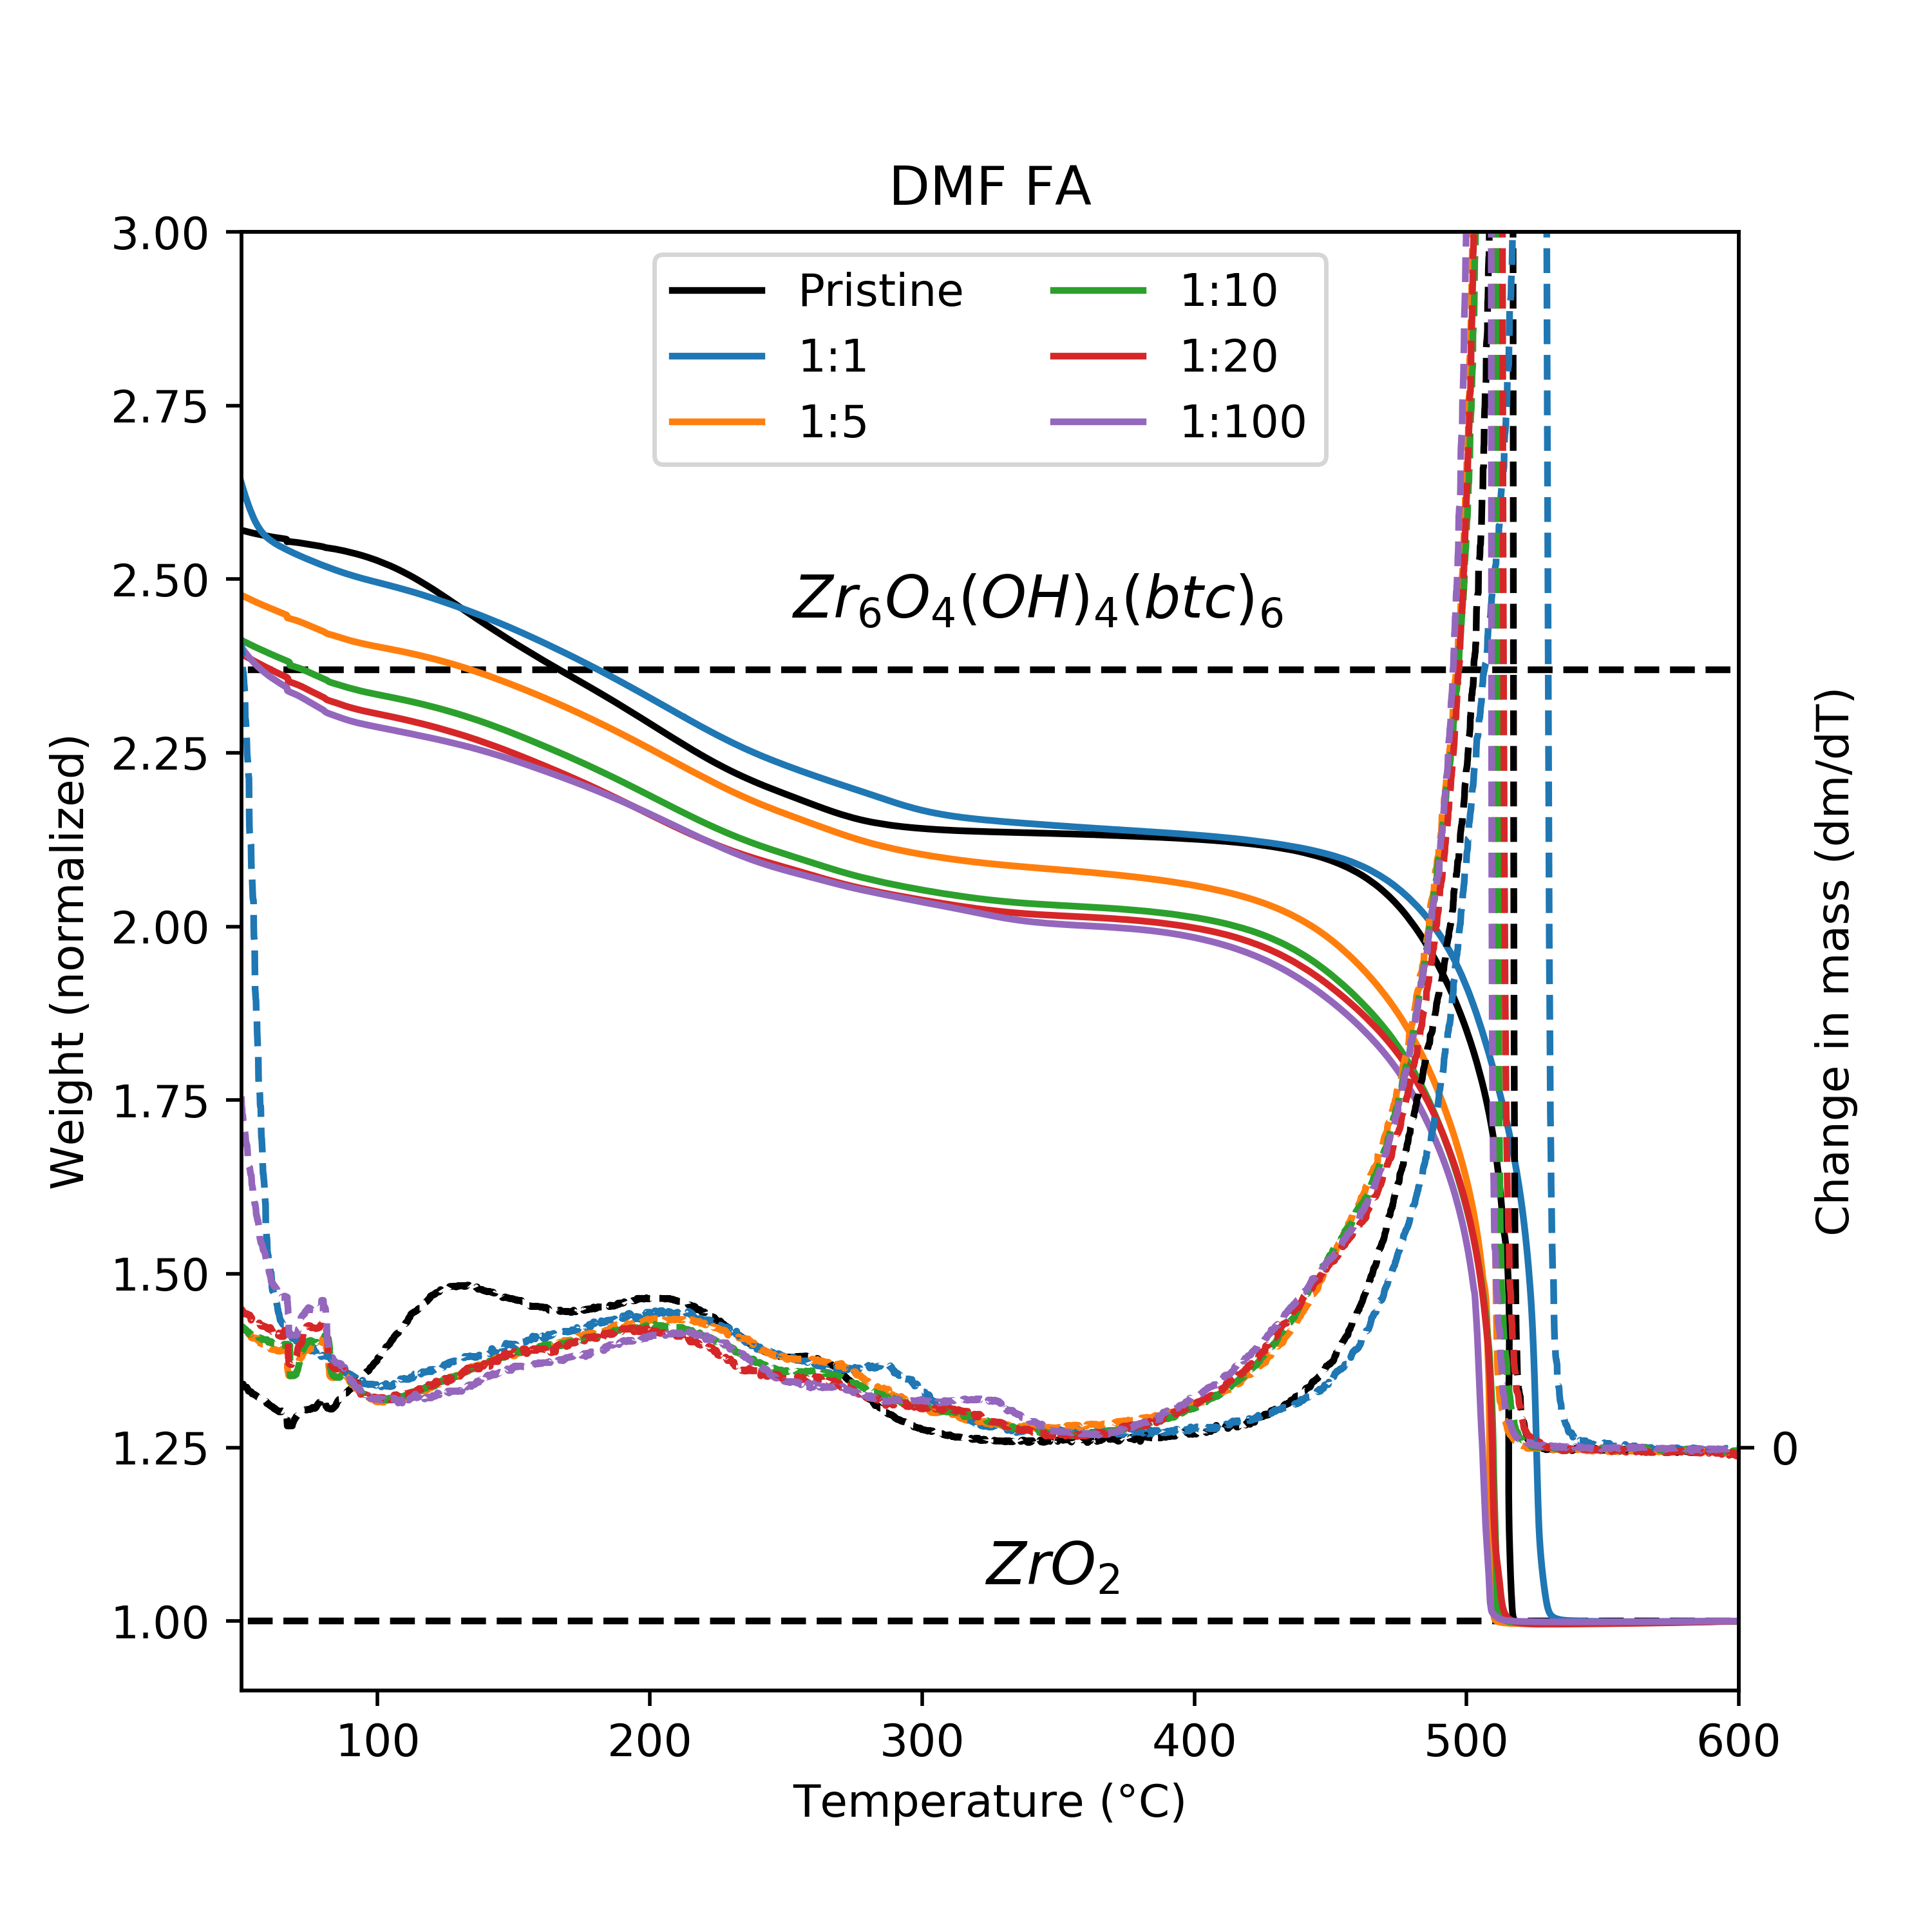
\includegraphics[width=\textwidth]{tga/DMF-FA}%
		\caption{}%
        \label{def:fgr:tga-dmf-fa}
    \end{subfigure}
    \begin{subfigure}{0.45\linewidth}
        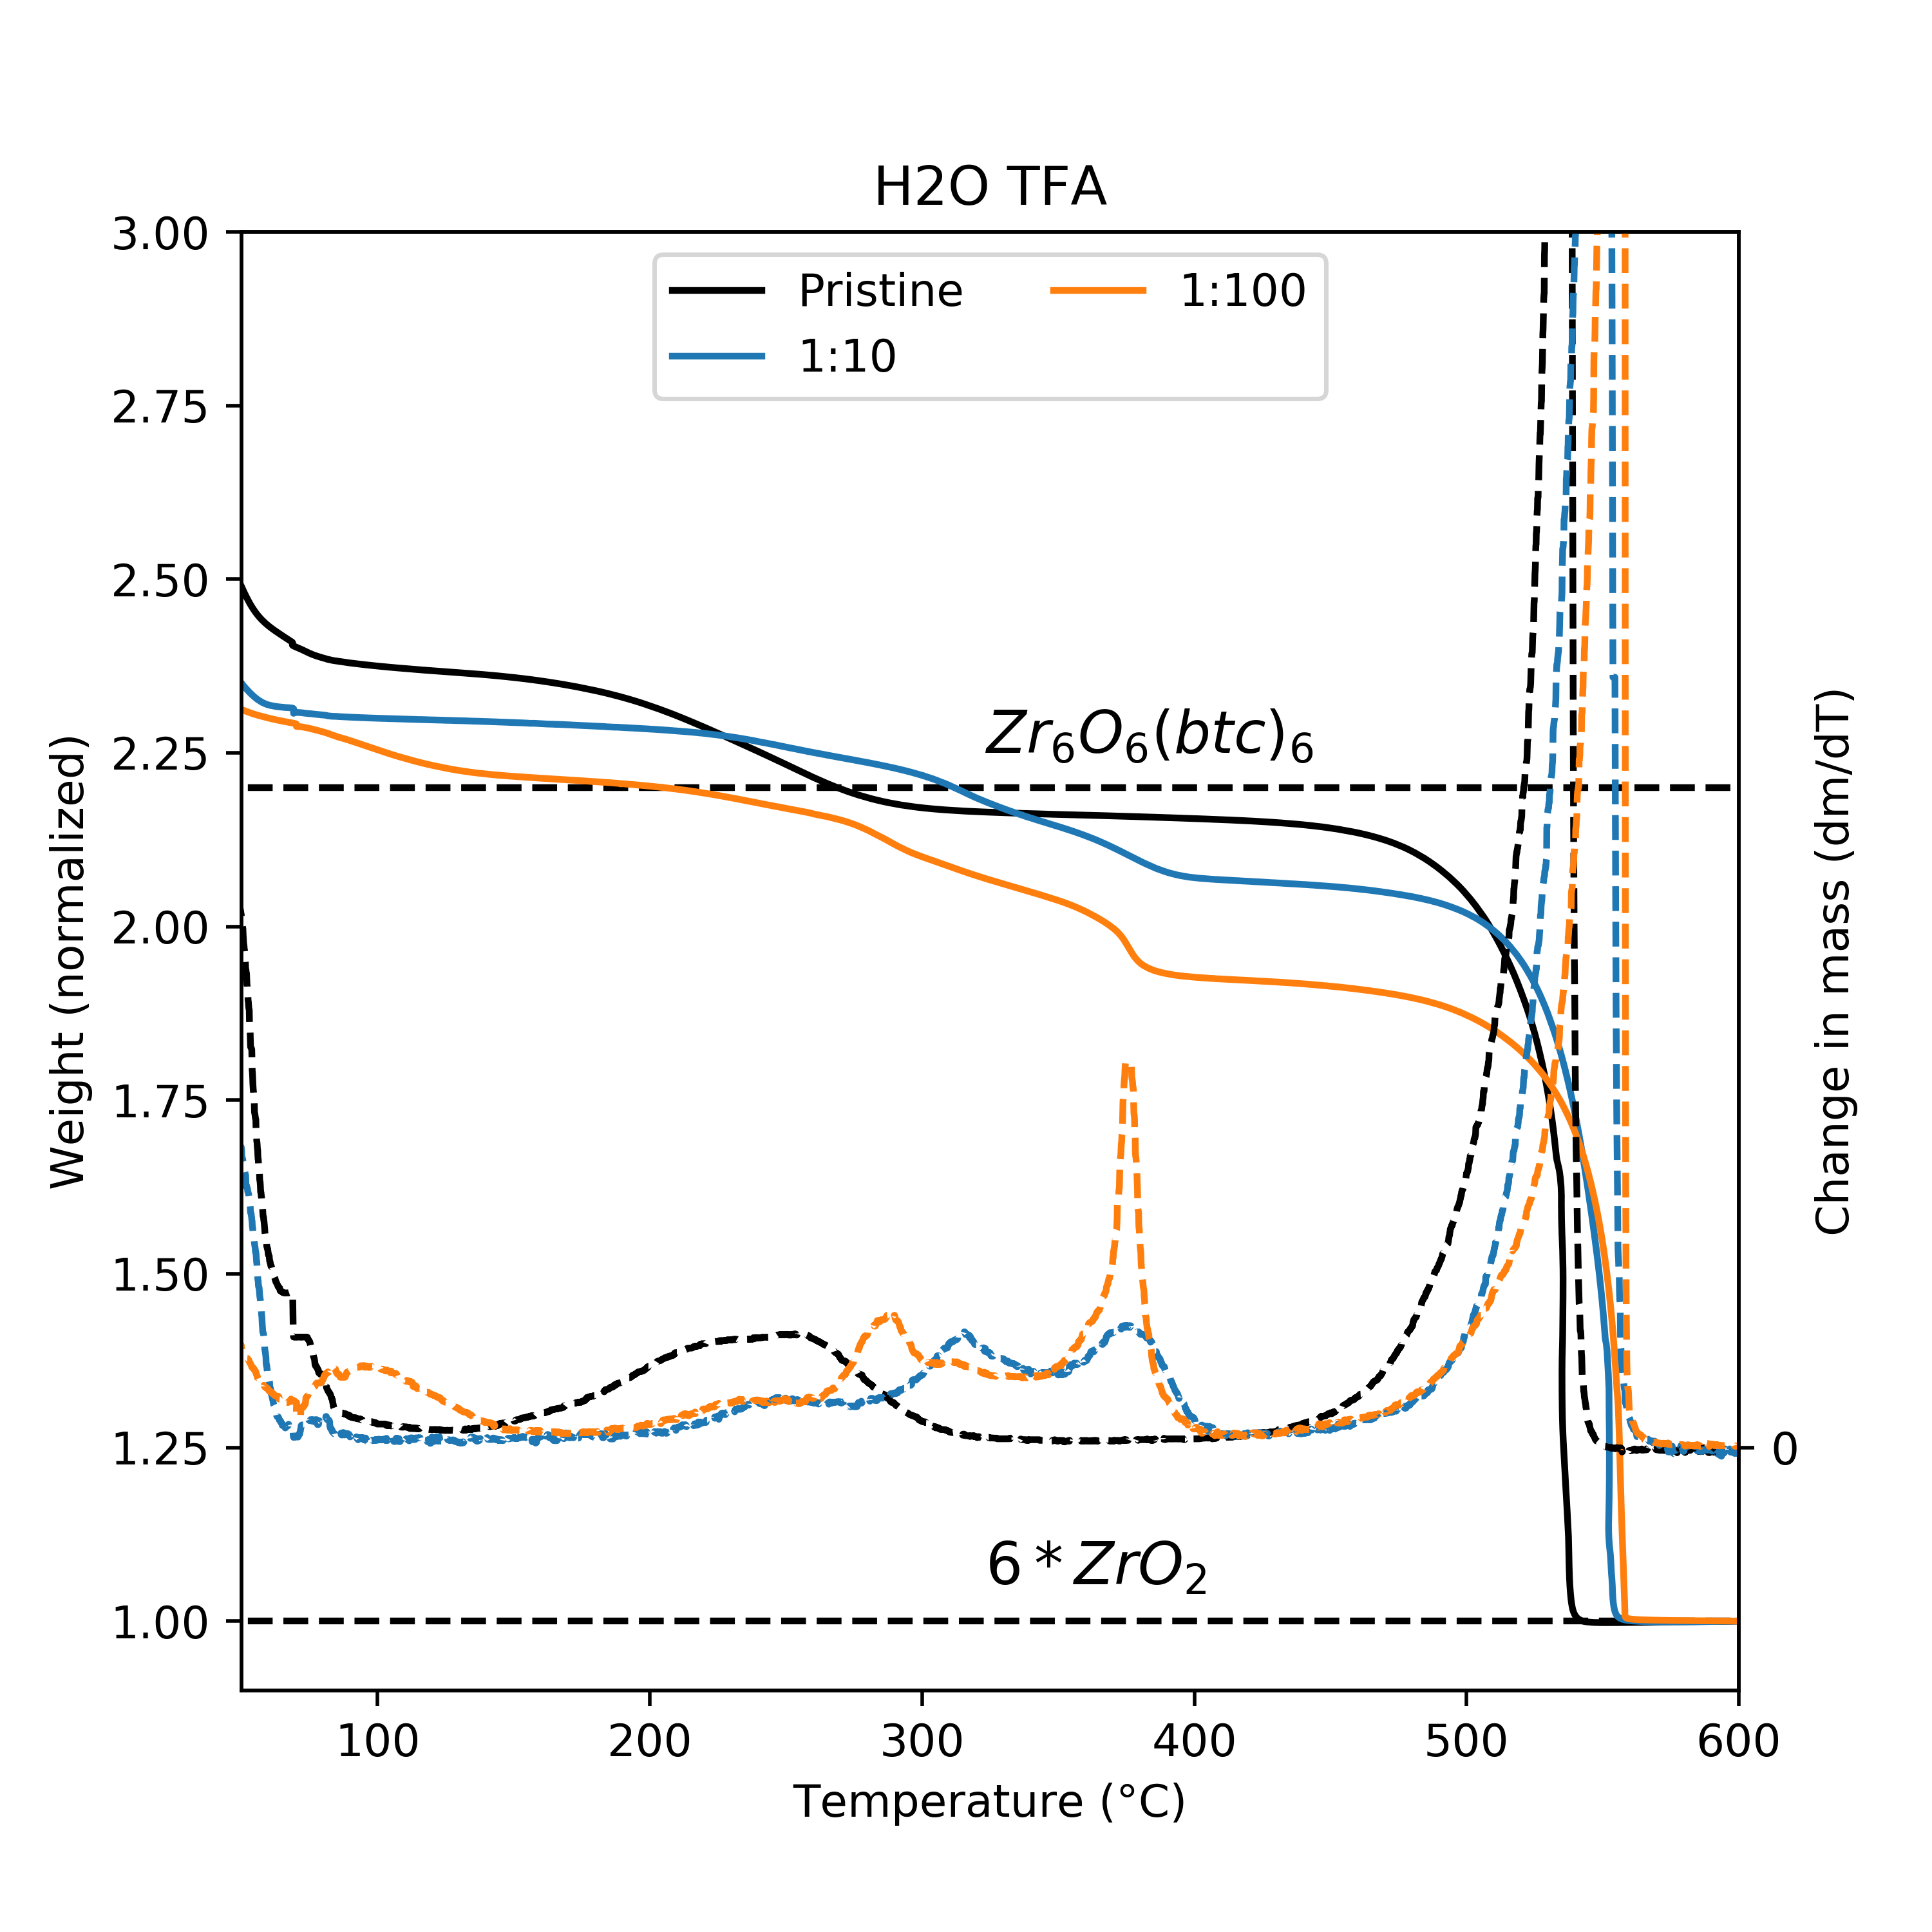
\includegraphics[width=\textwidth]{tga/H2O-TFA}%
		\caption{}%
        \label{def:fgr:tga-h2o-tfa}
    \end{subfigure}

    
    \begin{subfigure}{0.45\linewidth}
        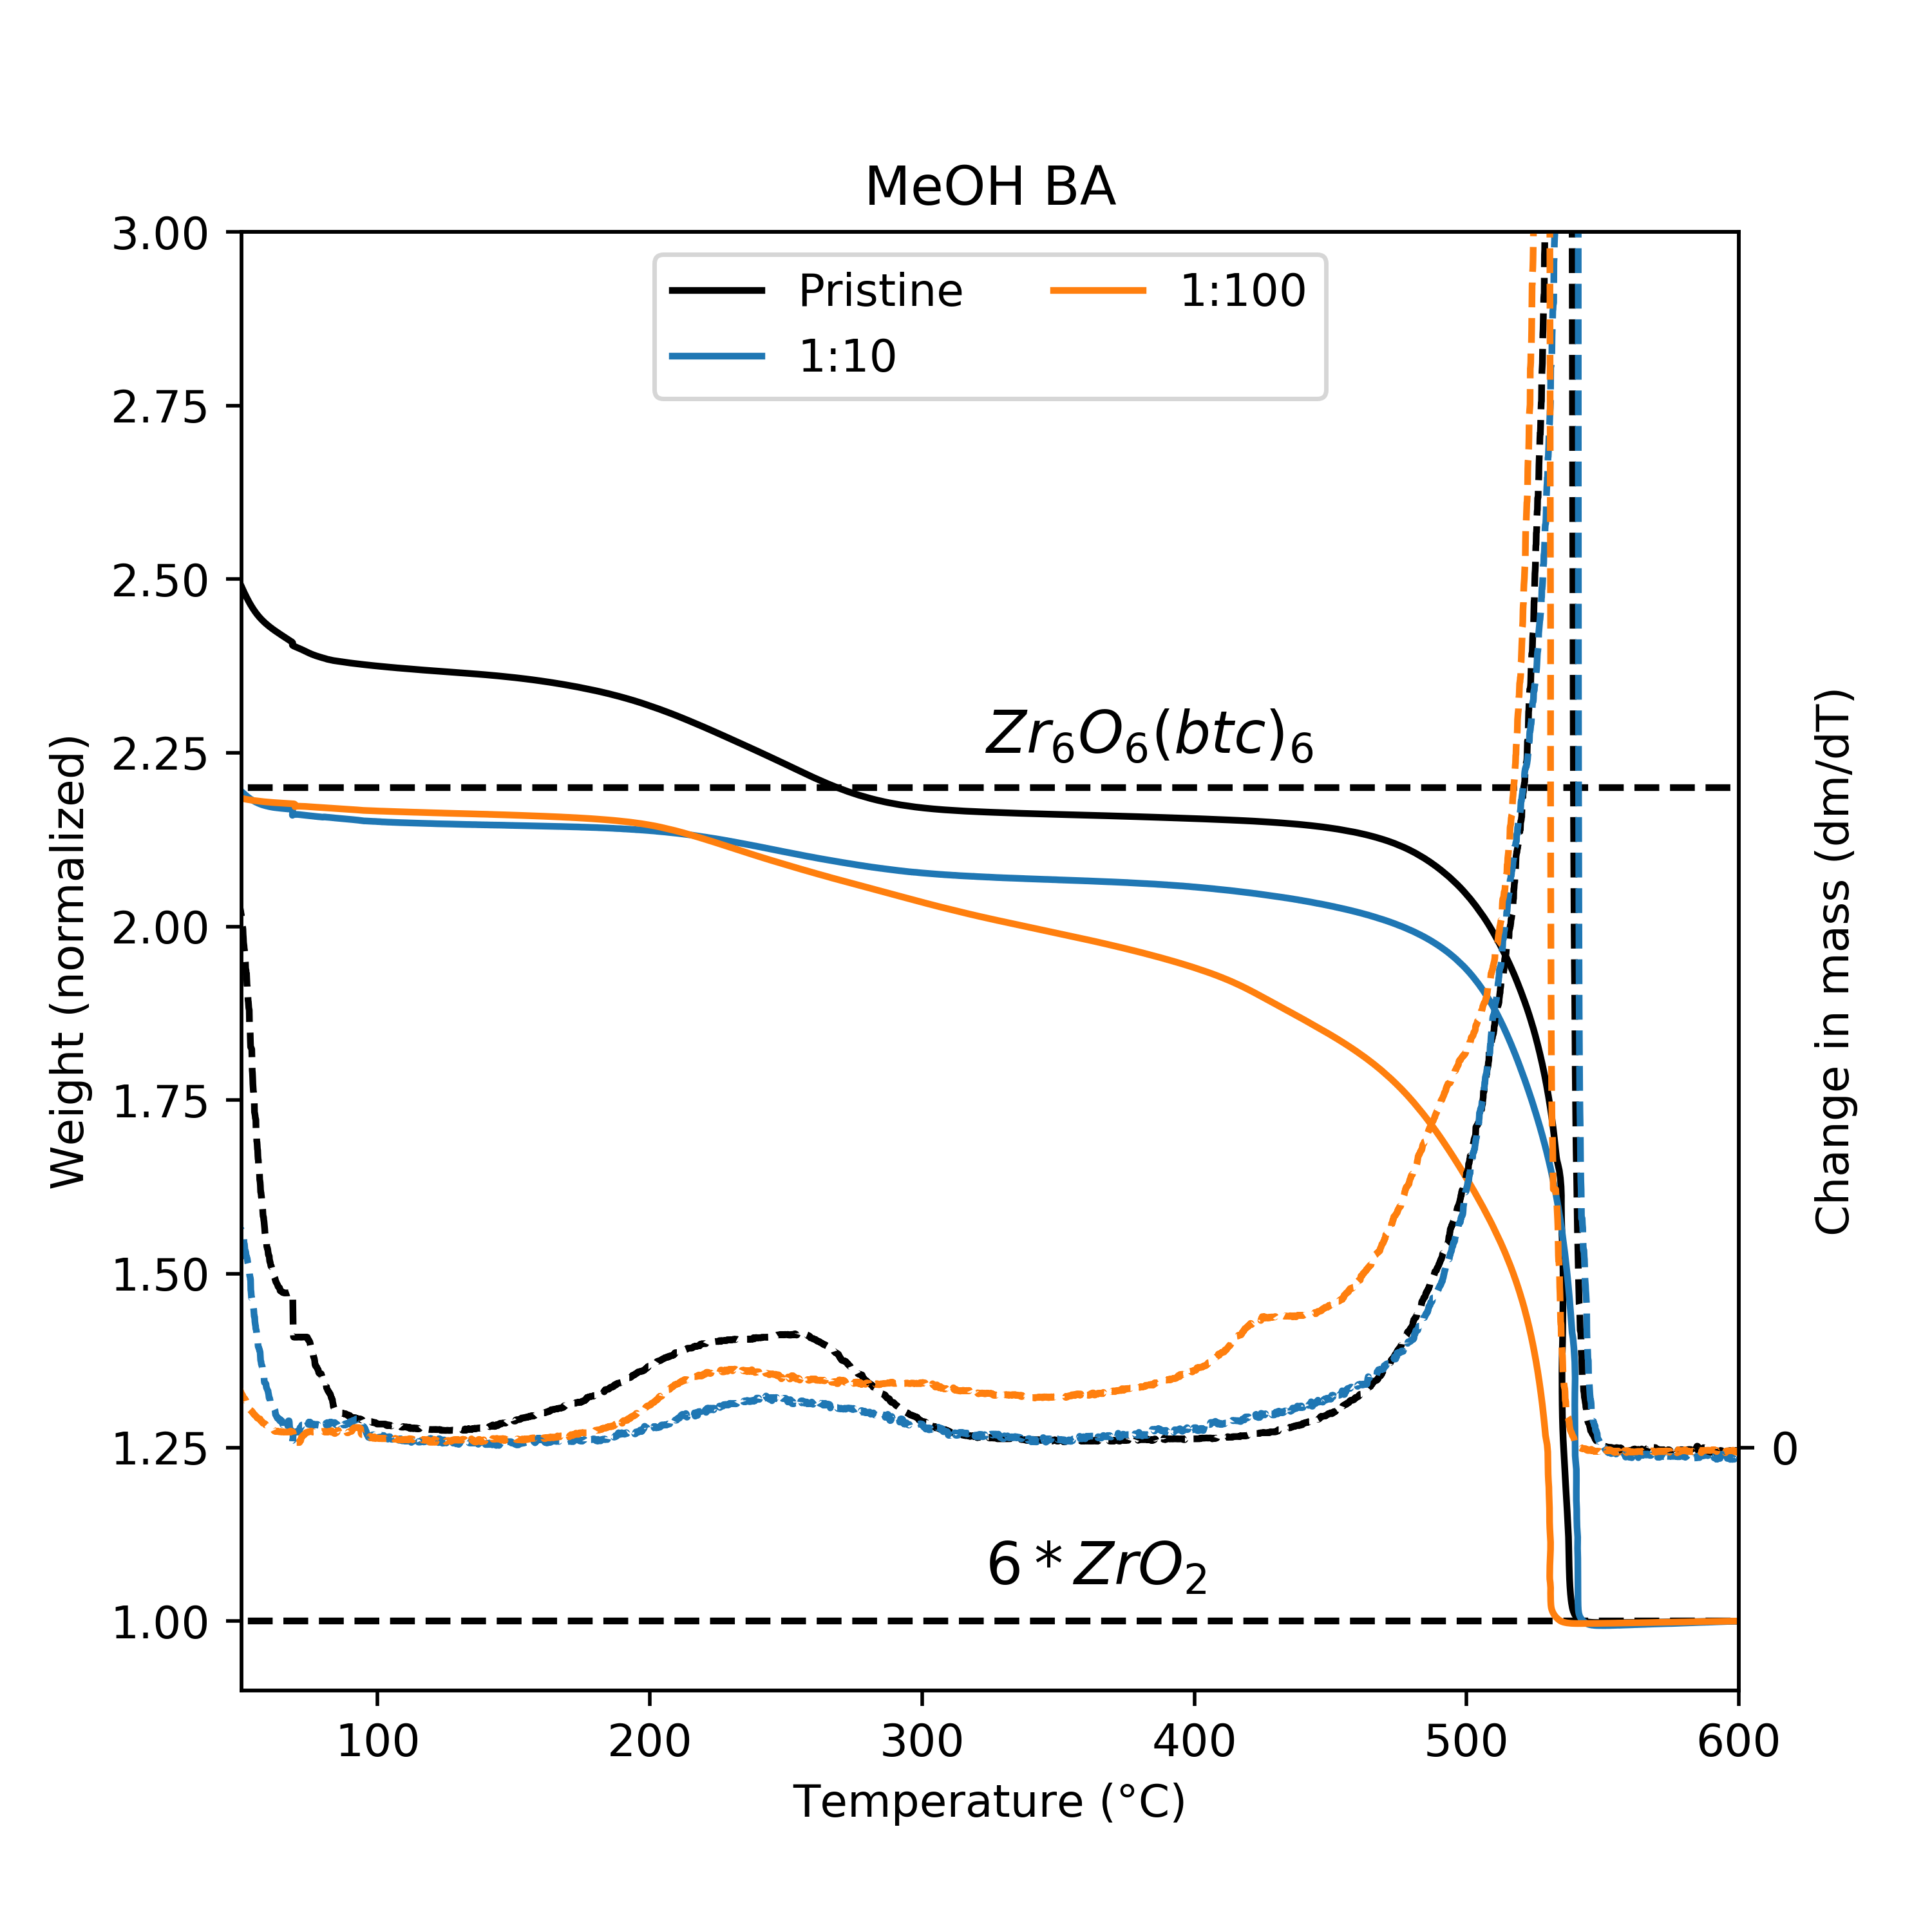
\includegraphics[width=\textwidth]{tga/MeOH-BA}%
		\caption{}%
        \label{def:fgr:tga-meoh-ba}
    \end{subfigure}
    \begin{subfigure}{0.45\linewidth}
        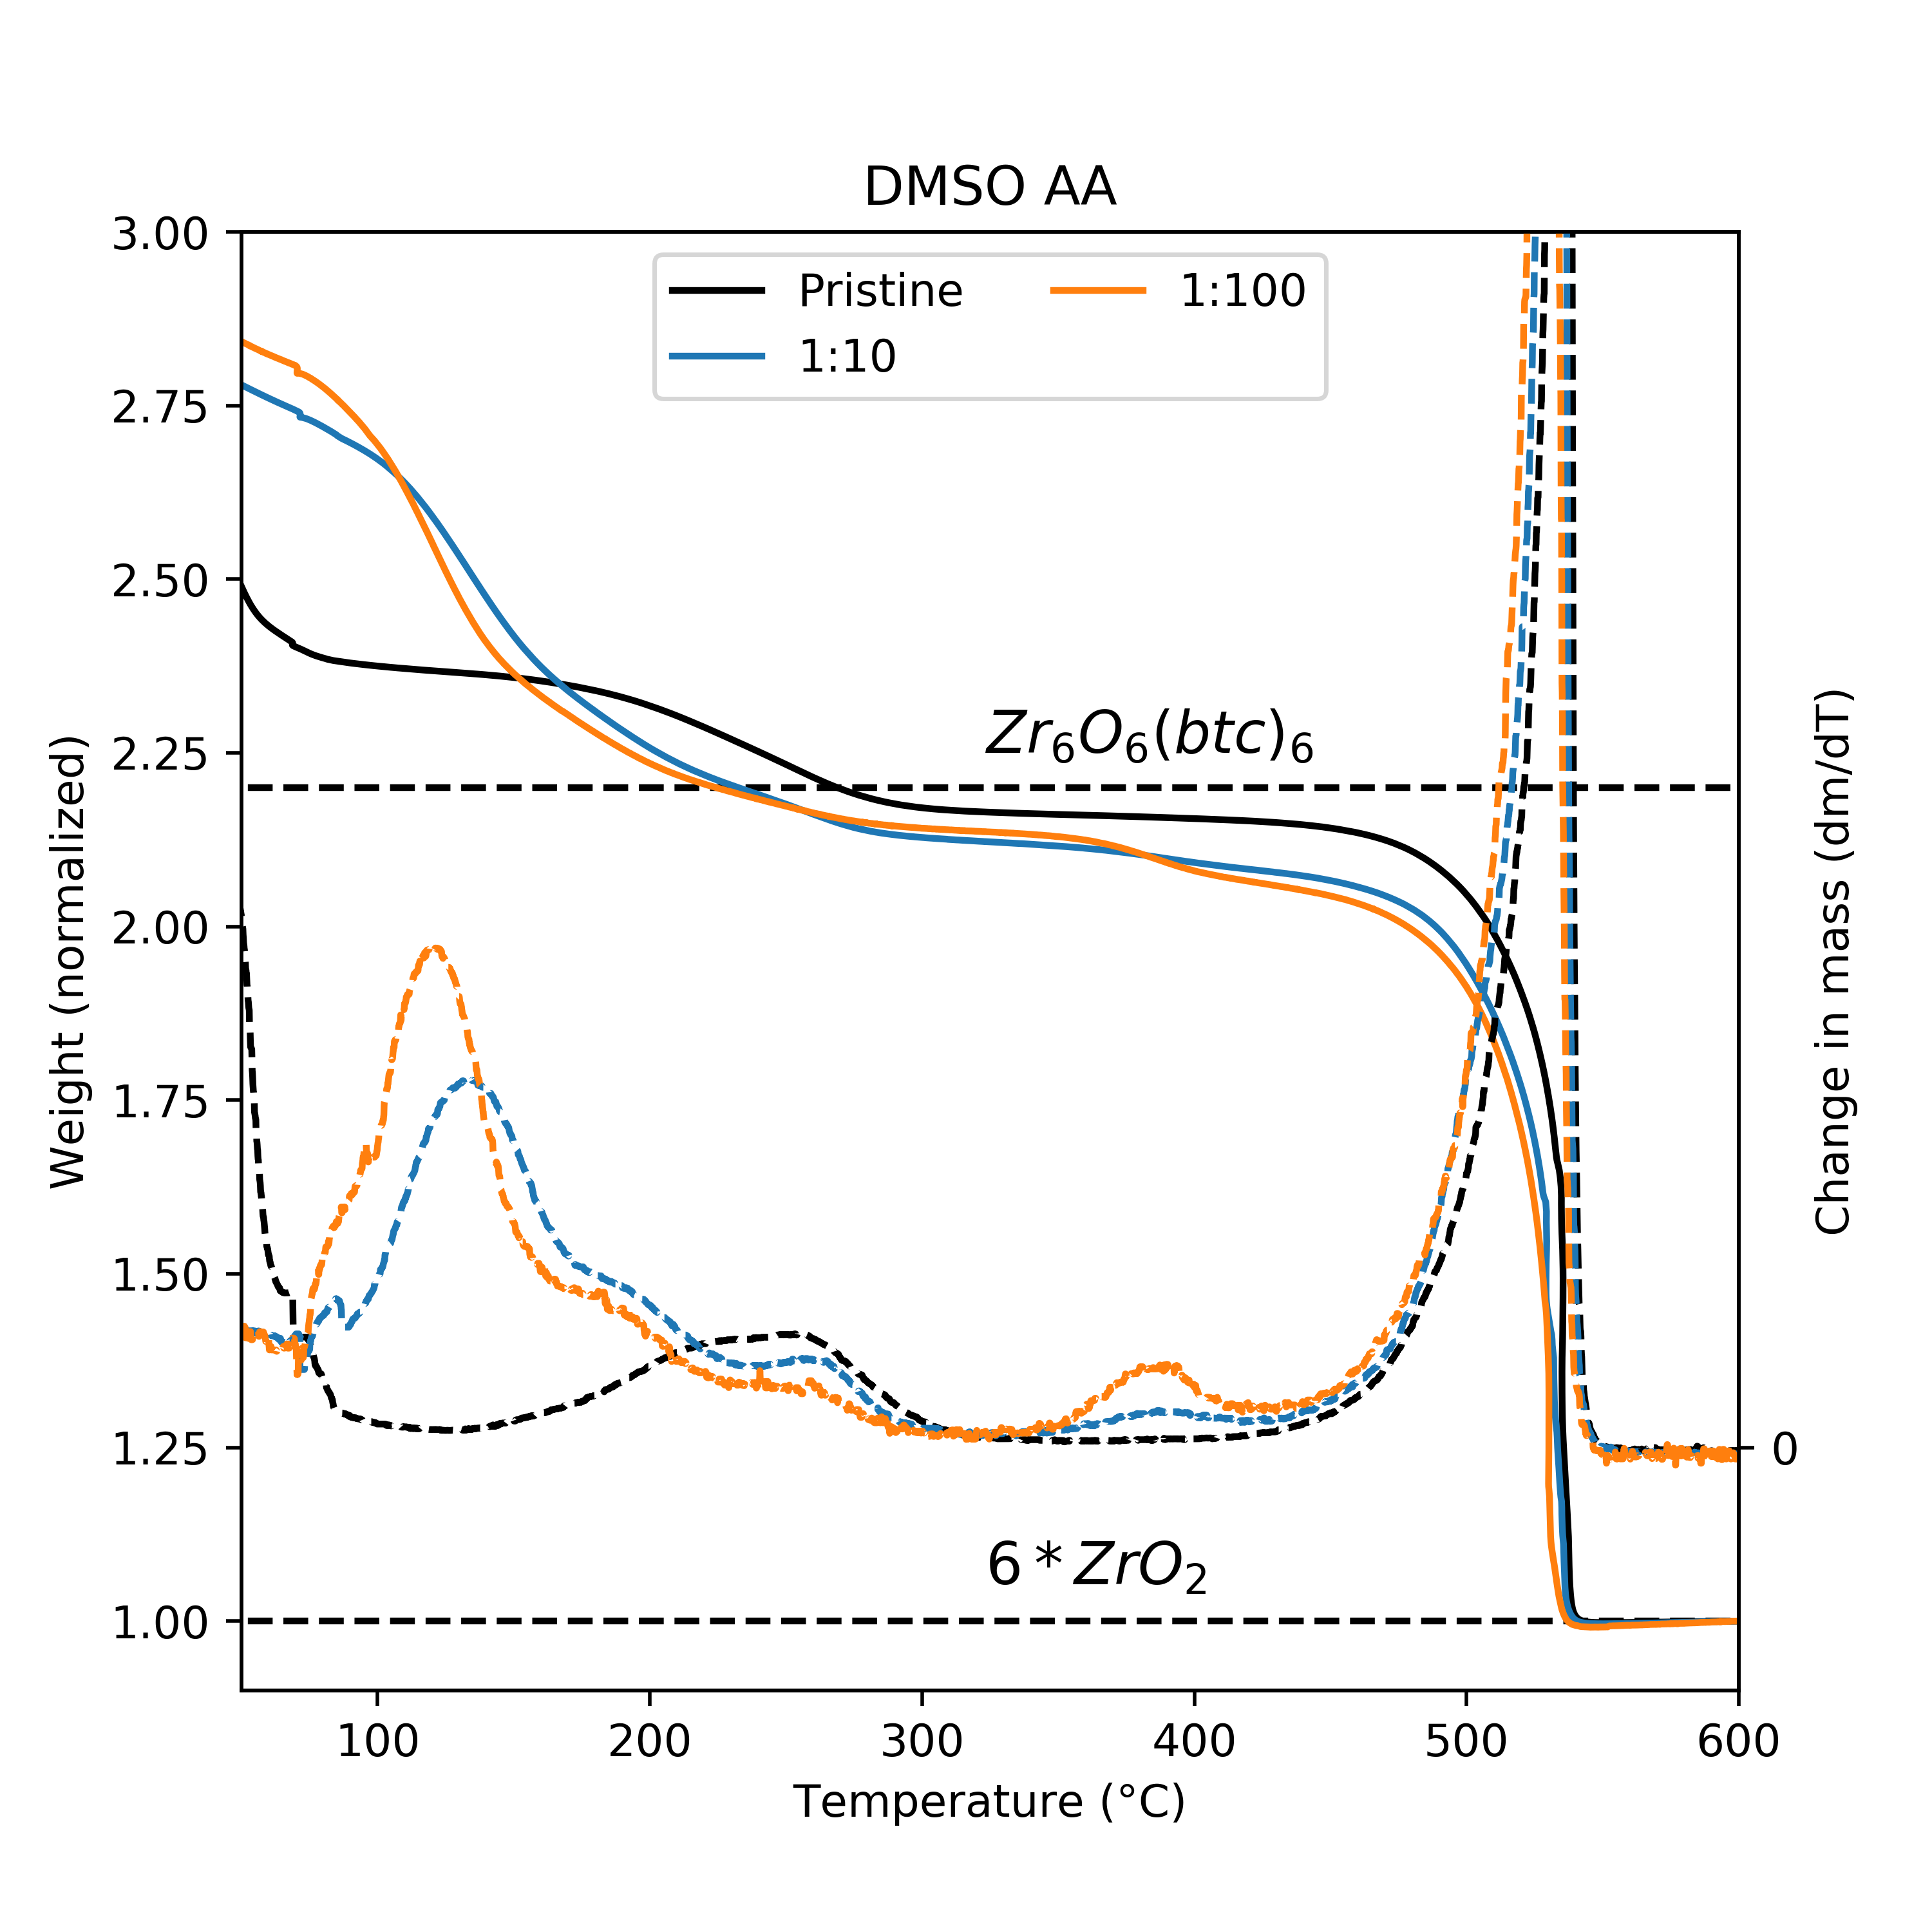
\includegraphics[width=\textwidth]{tga/DMSO-AA}%
		\caption{}%
        \label{def:fgr:tga-dmso-aa}
    \end{subfigure}

    \caption{A selection of the TGA curves as measured on the
    leached samples: (a) formic acid in DMF, (b) trifluoroacetic
    acid in water, (c) benzoic acid in methanol and (d) acetic acid
    in DMSO. The curve for the parent material is in black. 
    Dotted lines correspond to the secondary y axis as a 
    semilogarithm of the first derivative of mass loss with 
    respect to temperature.}%
    \label{def:fgr:tga-dataset}
\end{figure}

In leached samples where other acids were present,
it is likely that the original formate capping the defects 
has been replaced with an acid molecule from solution,
purely through kinetic means due to the large excess.
As evidenced in \autoref{def:fgr:tga-defects}, the mass 
loss corresponding to the formate is reduced, or no longer present. 
Acetic acid (\autoref{def:fgr:tga-dmso-aa}) leaves the 
structure at a higher temperature, as 
a new peak is present at \SI{390}{\degreeCelsius}.
Benzoic acid (\autoref{def:fgr:tga-meoh-ba}) introduces a progressive 
mass loss near the total decomposition temperature of \SI{550}{\degreeCelsius}.
As it is similar to the btc linker, its higher stability
is not surprising. Finally, the samples leached with 
TFA have a more complicated curve, with two or even 
three peaks in the derivative with respect to temperature.

The solvent used can be removed in all cases before 
\SI{200}{\degreeCelsius}. DMSO is the one with the highest
preponderence in the leached samples (\autoref{def:fgr:tga-dmso-aa}) 
and the most difficult to remove, likely due to its high boiling point.

The graphs in \autoref{def:fgr:tga-defects} summarize the 
trends in missing linker defects as calculated through 
the plateau at \SI{420}{\degreeCelsius}. Several clear trends can be 


\begin{figure}[htb]
    \centering

    \begin{subfigure}{0.45\linewidth}
        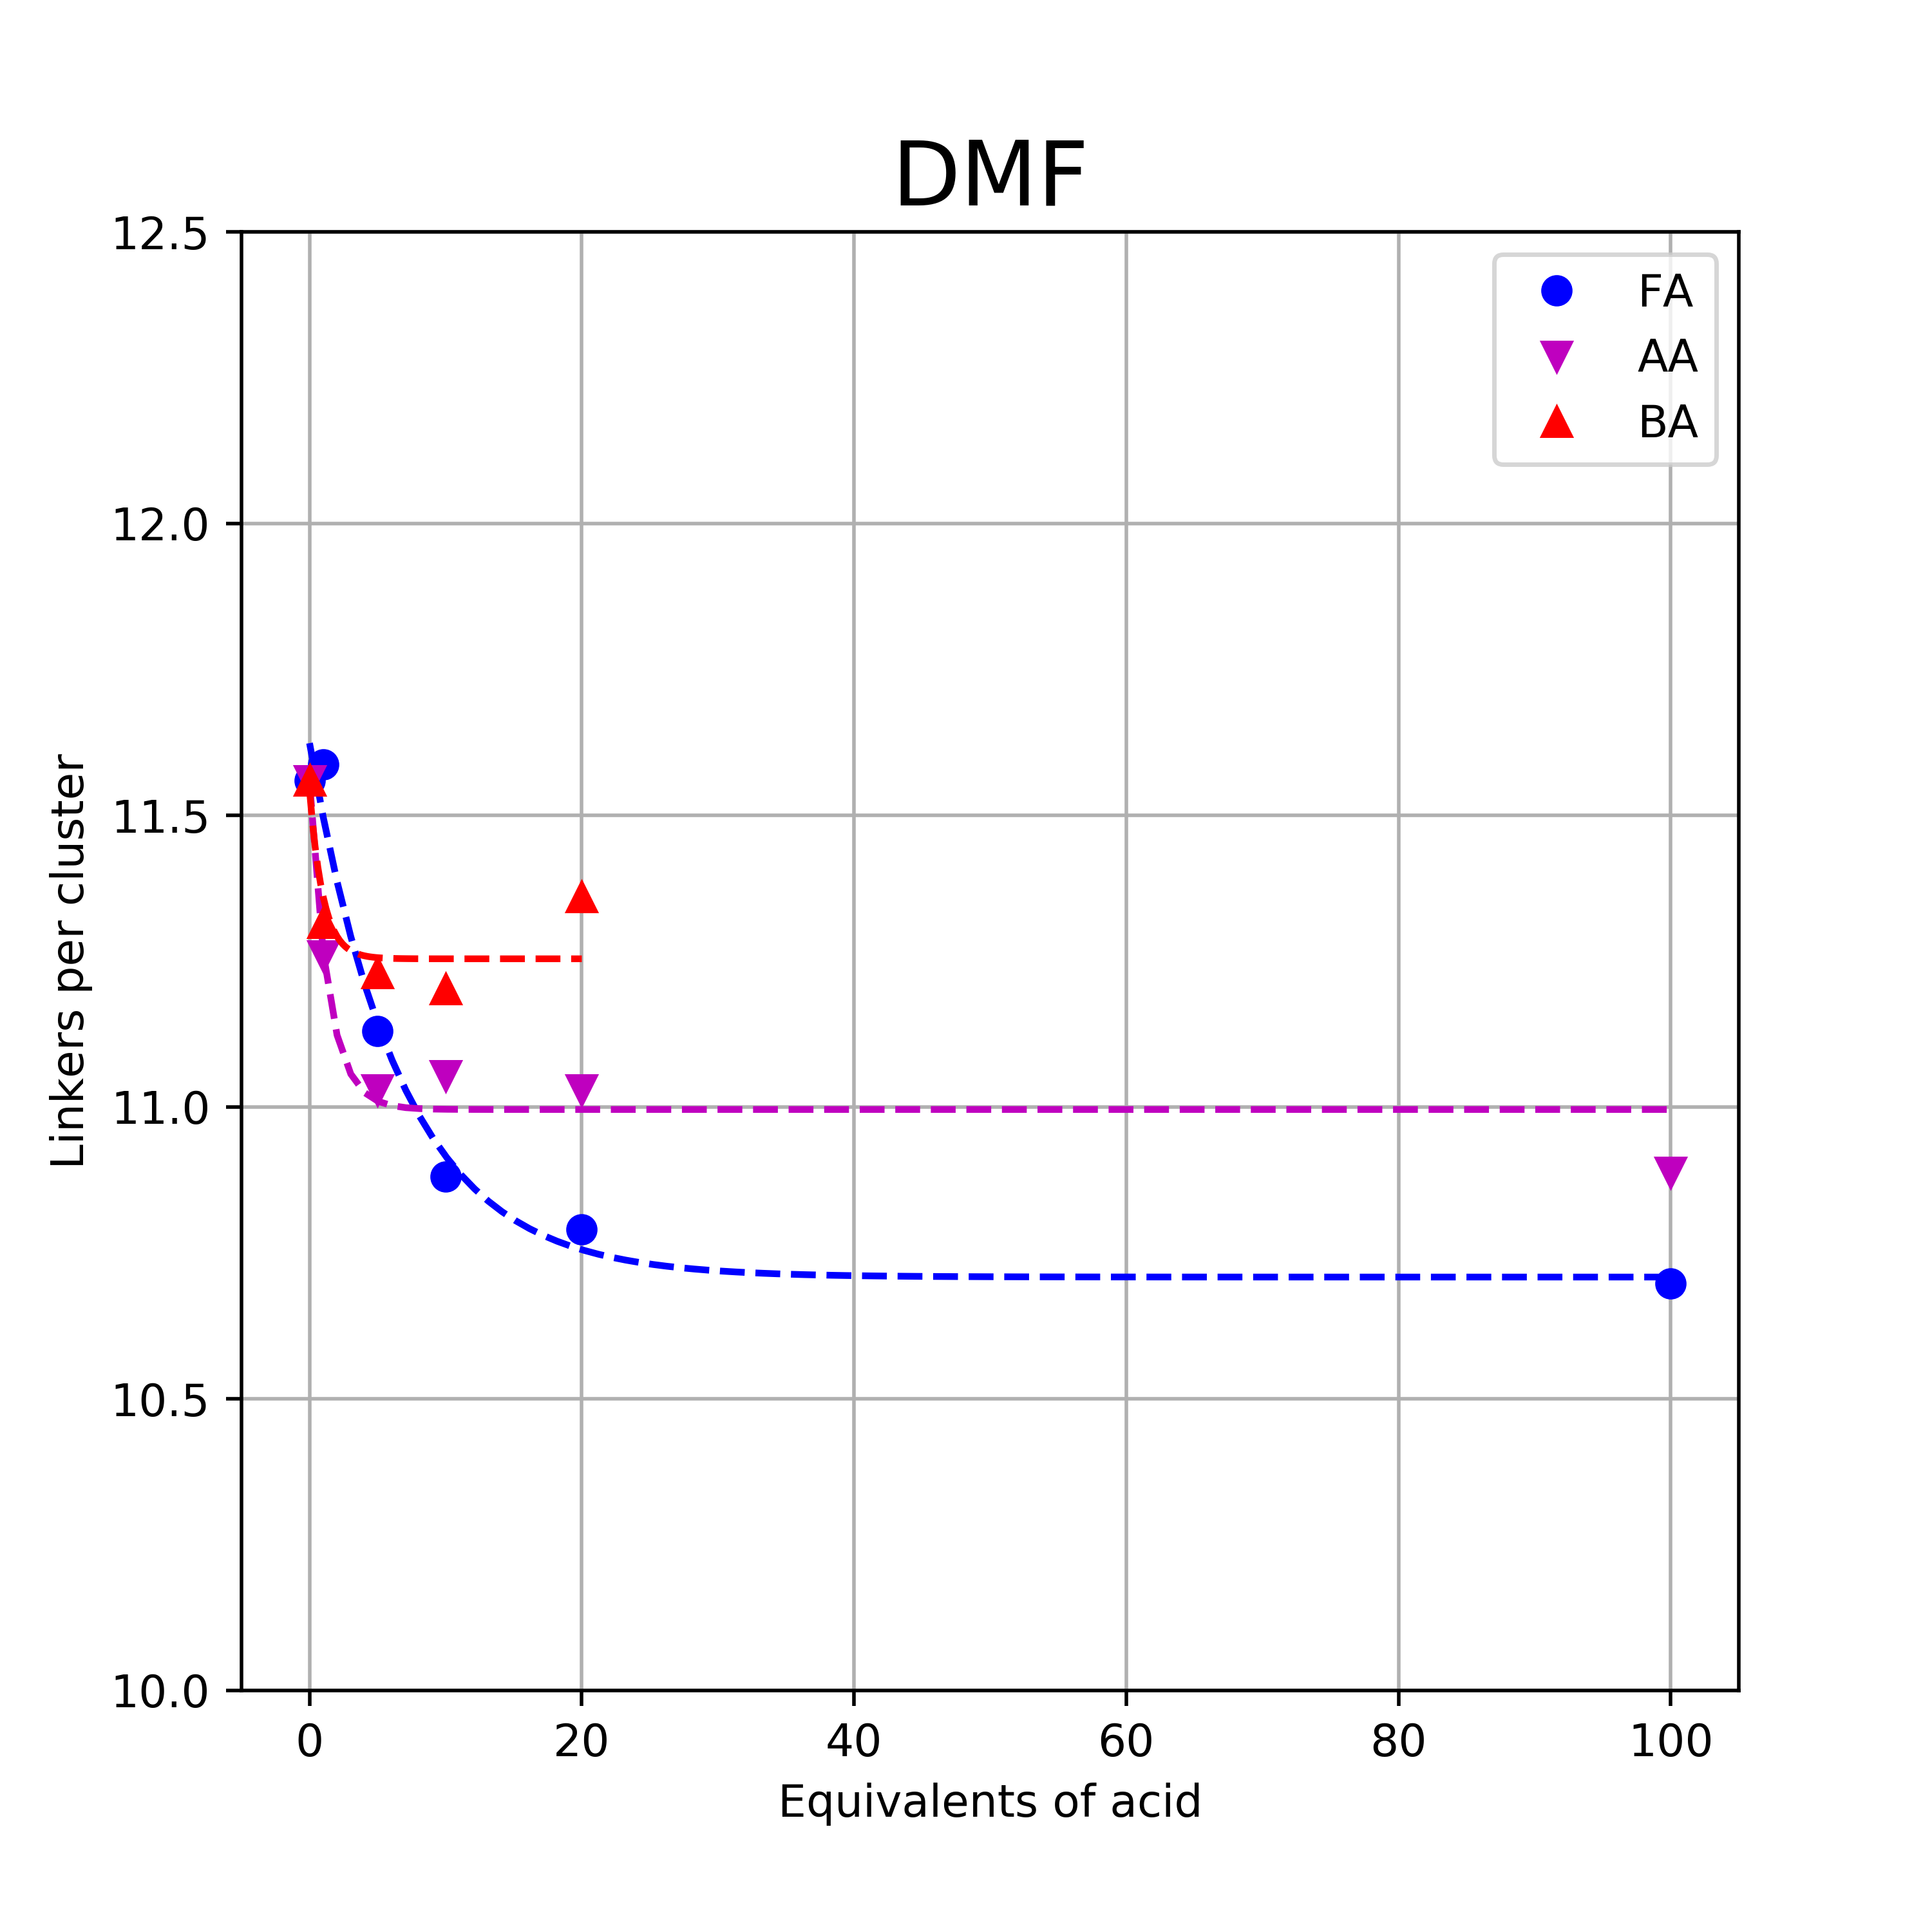
\includegraphics[width=\textwidth]{tga/DMF-def-overview}%
        \label{def:fgr:tga-dmf-linkers}
    \end{subfigure}
    \begin{subfigure}{0.45\linewidth}
        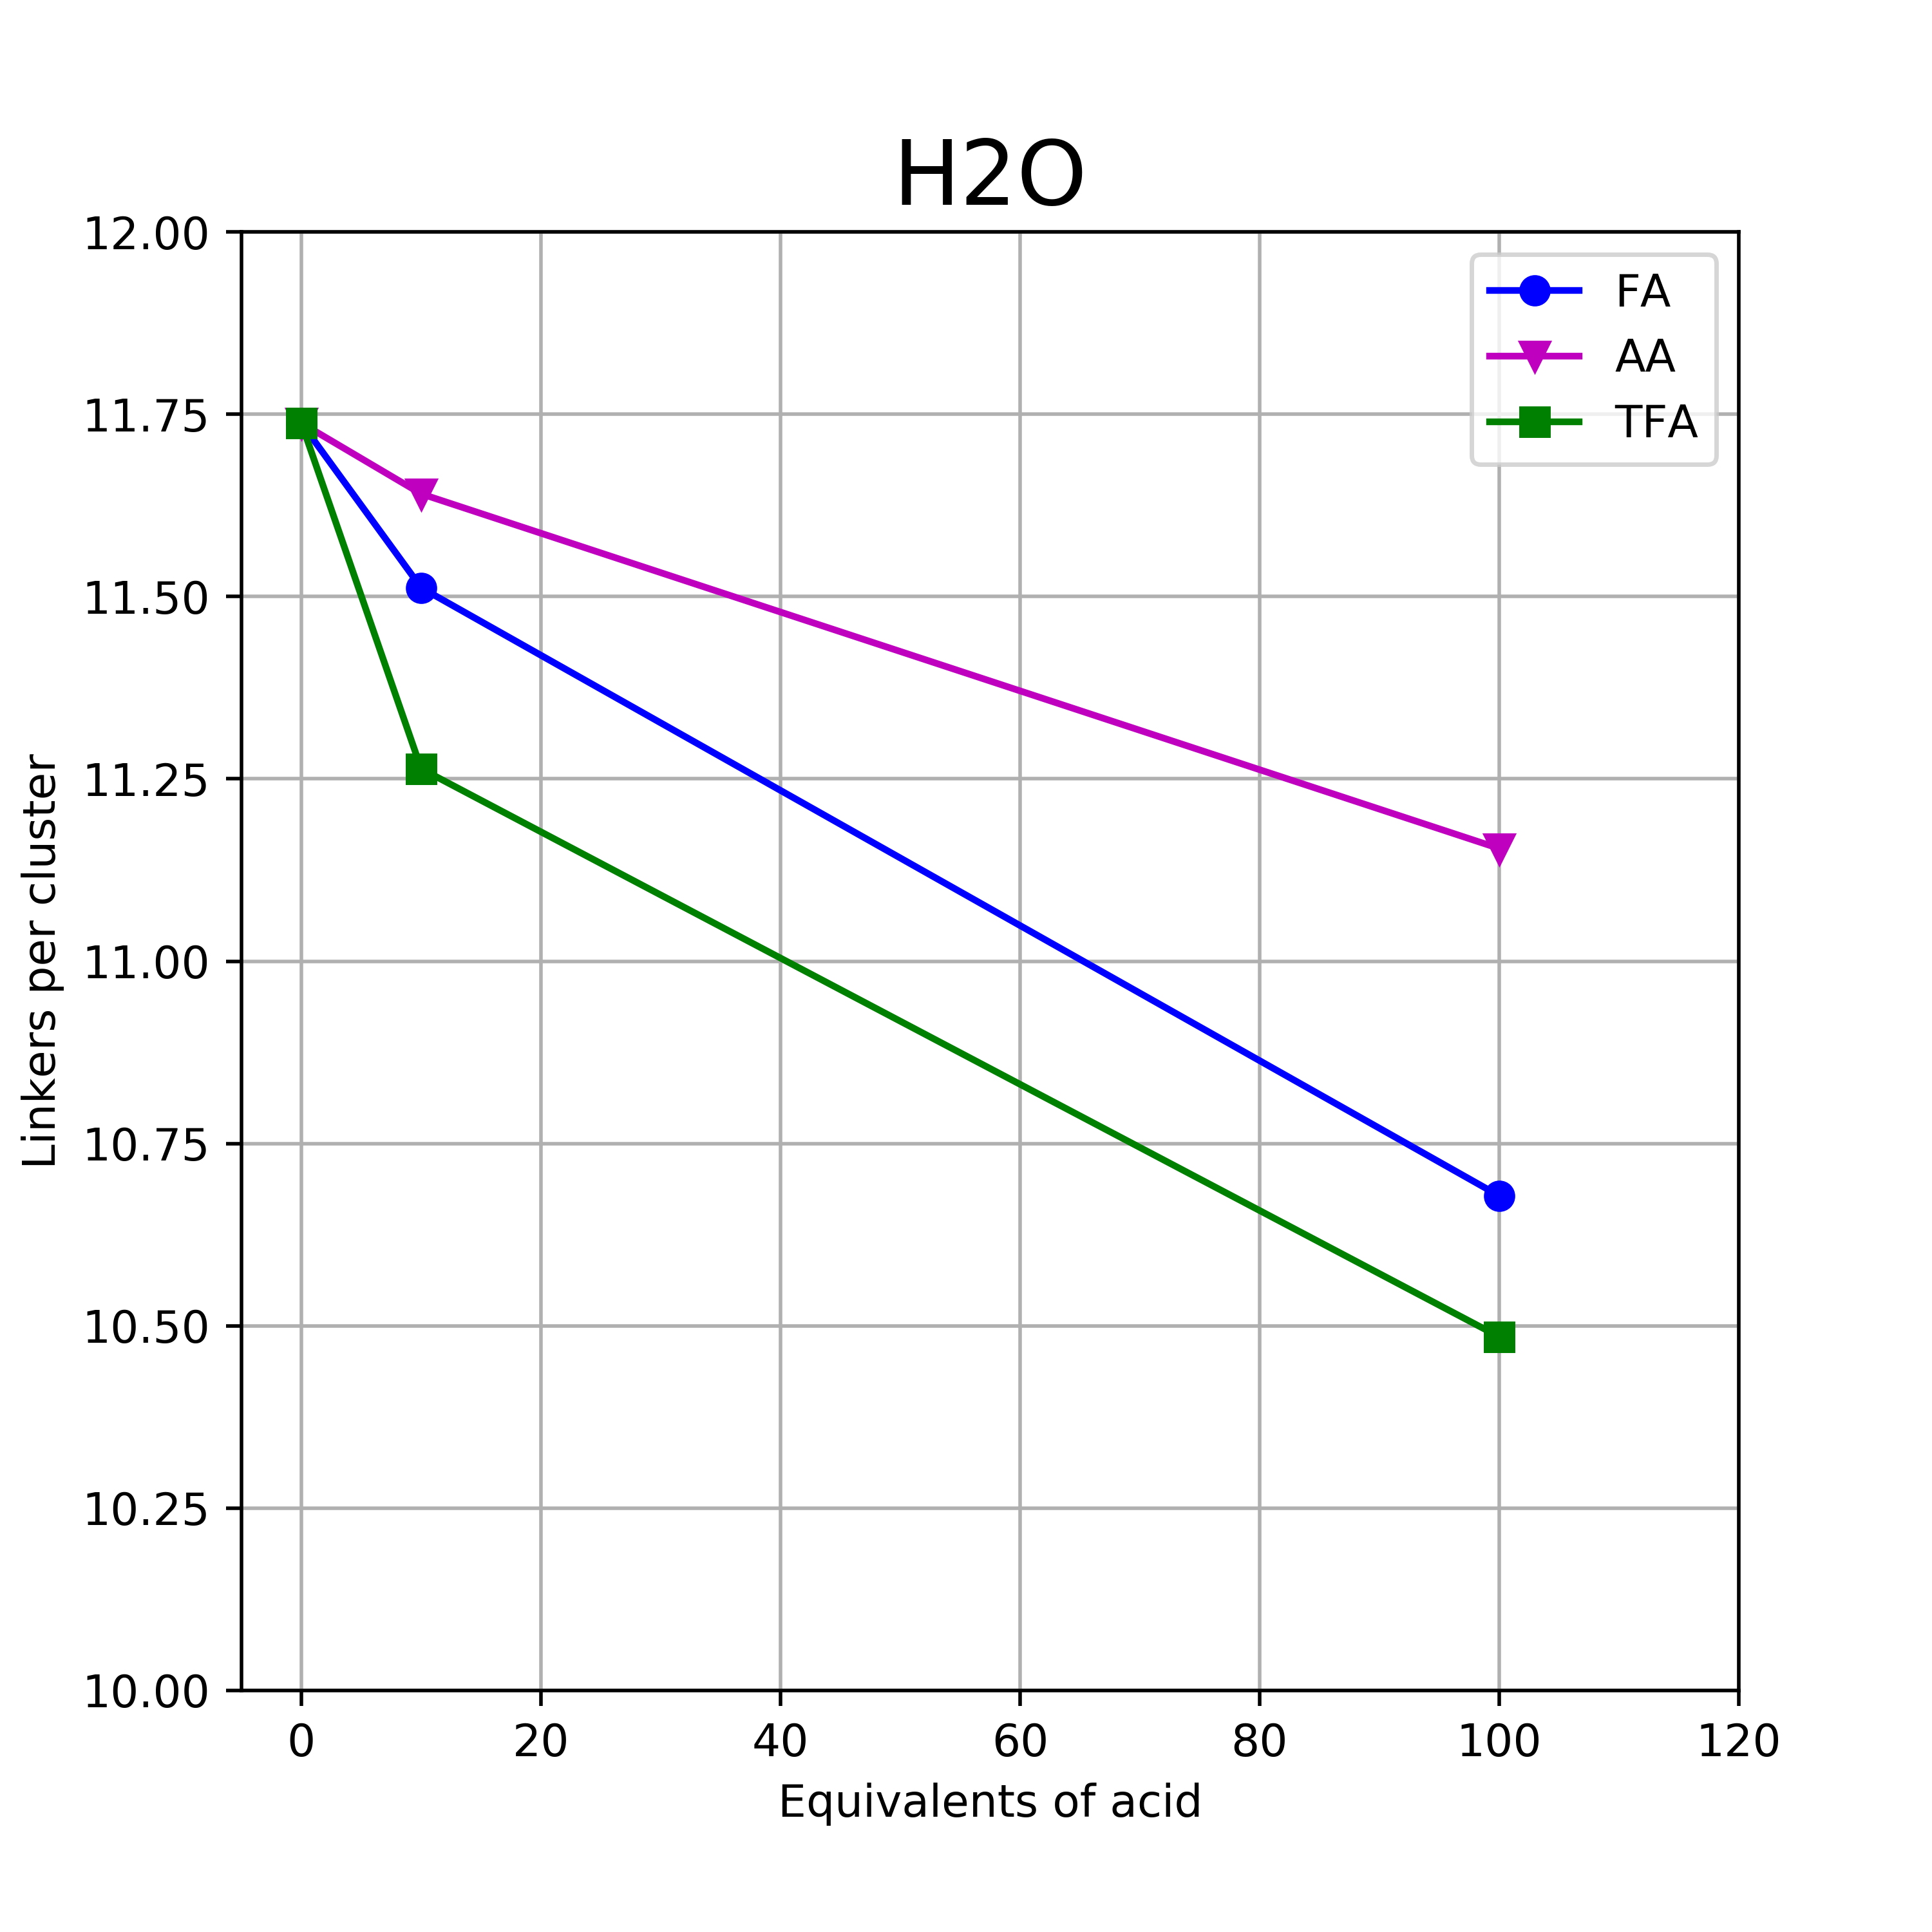
\includegraphics[width=\textwidth]{tga/H2O-def-overview}%
        \label{def:fgr:tga-h2o-linkers}
    \end{subfigure}

    
    \begin{subfigure}{0.45\linewidth}
        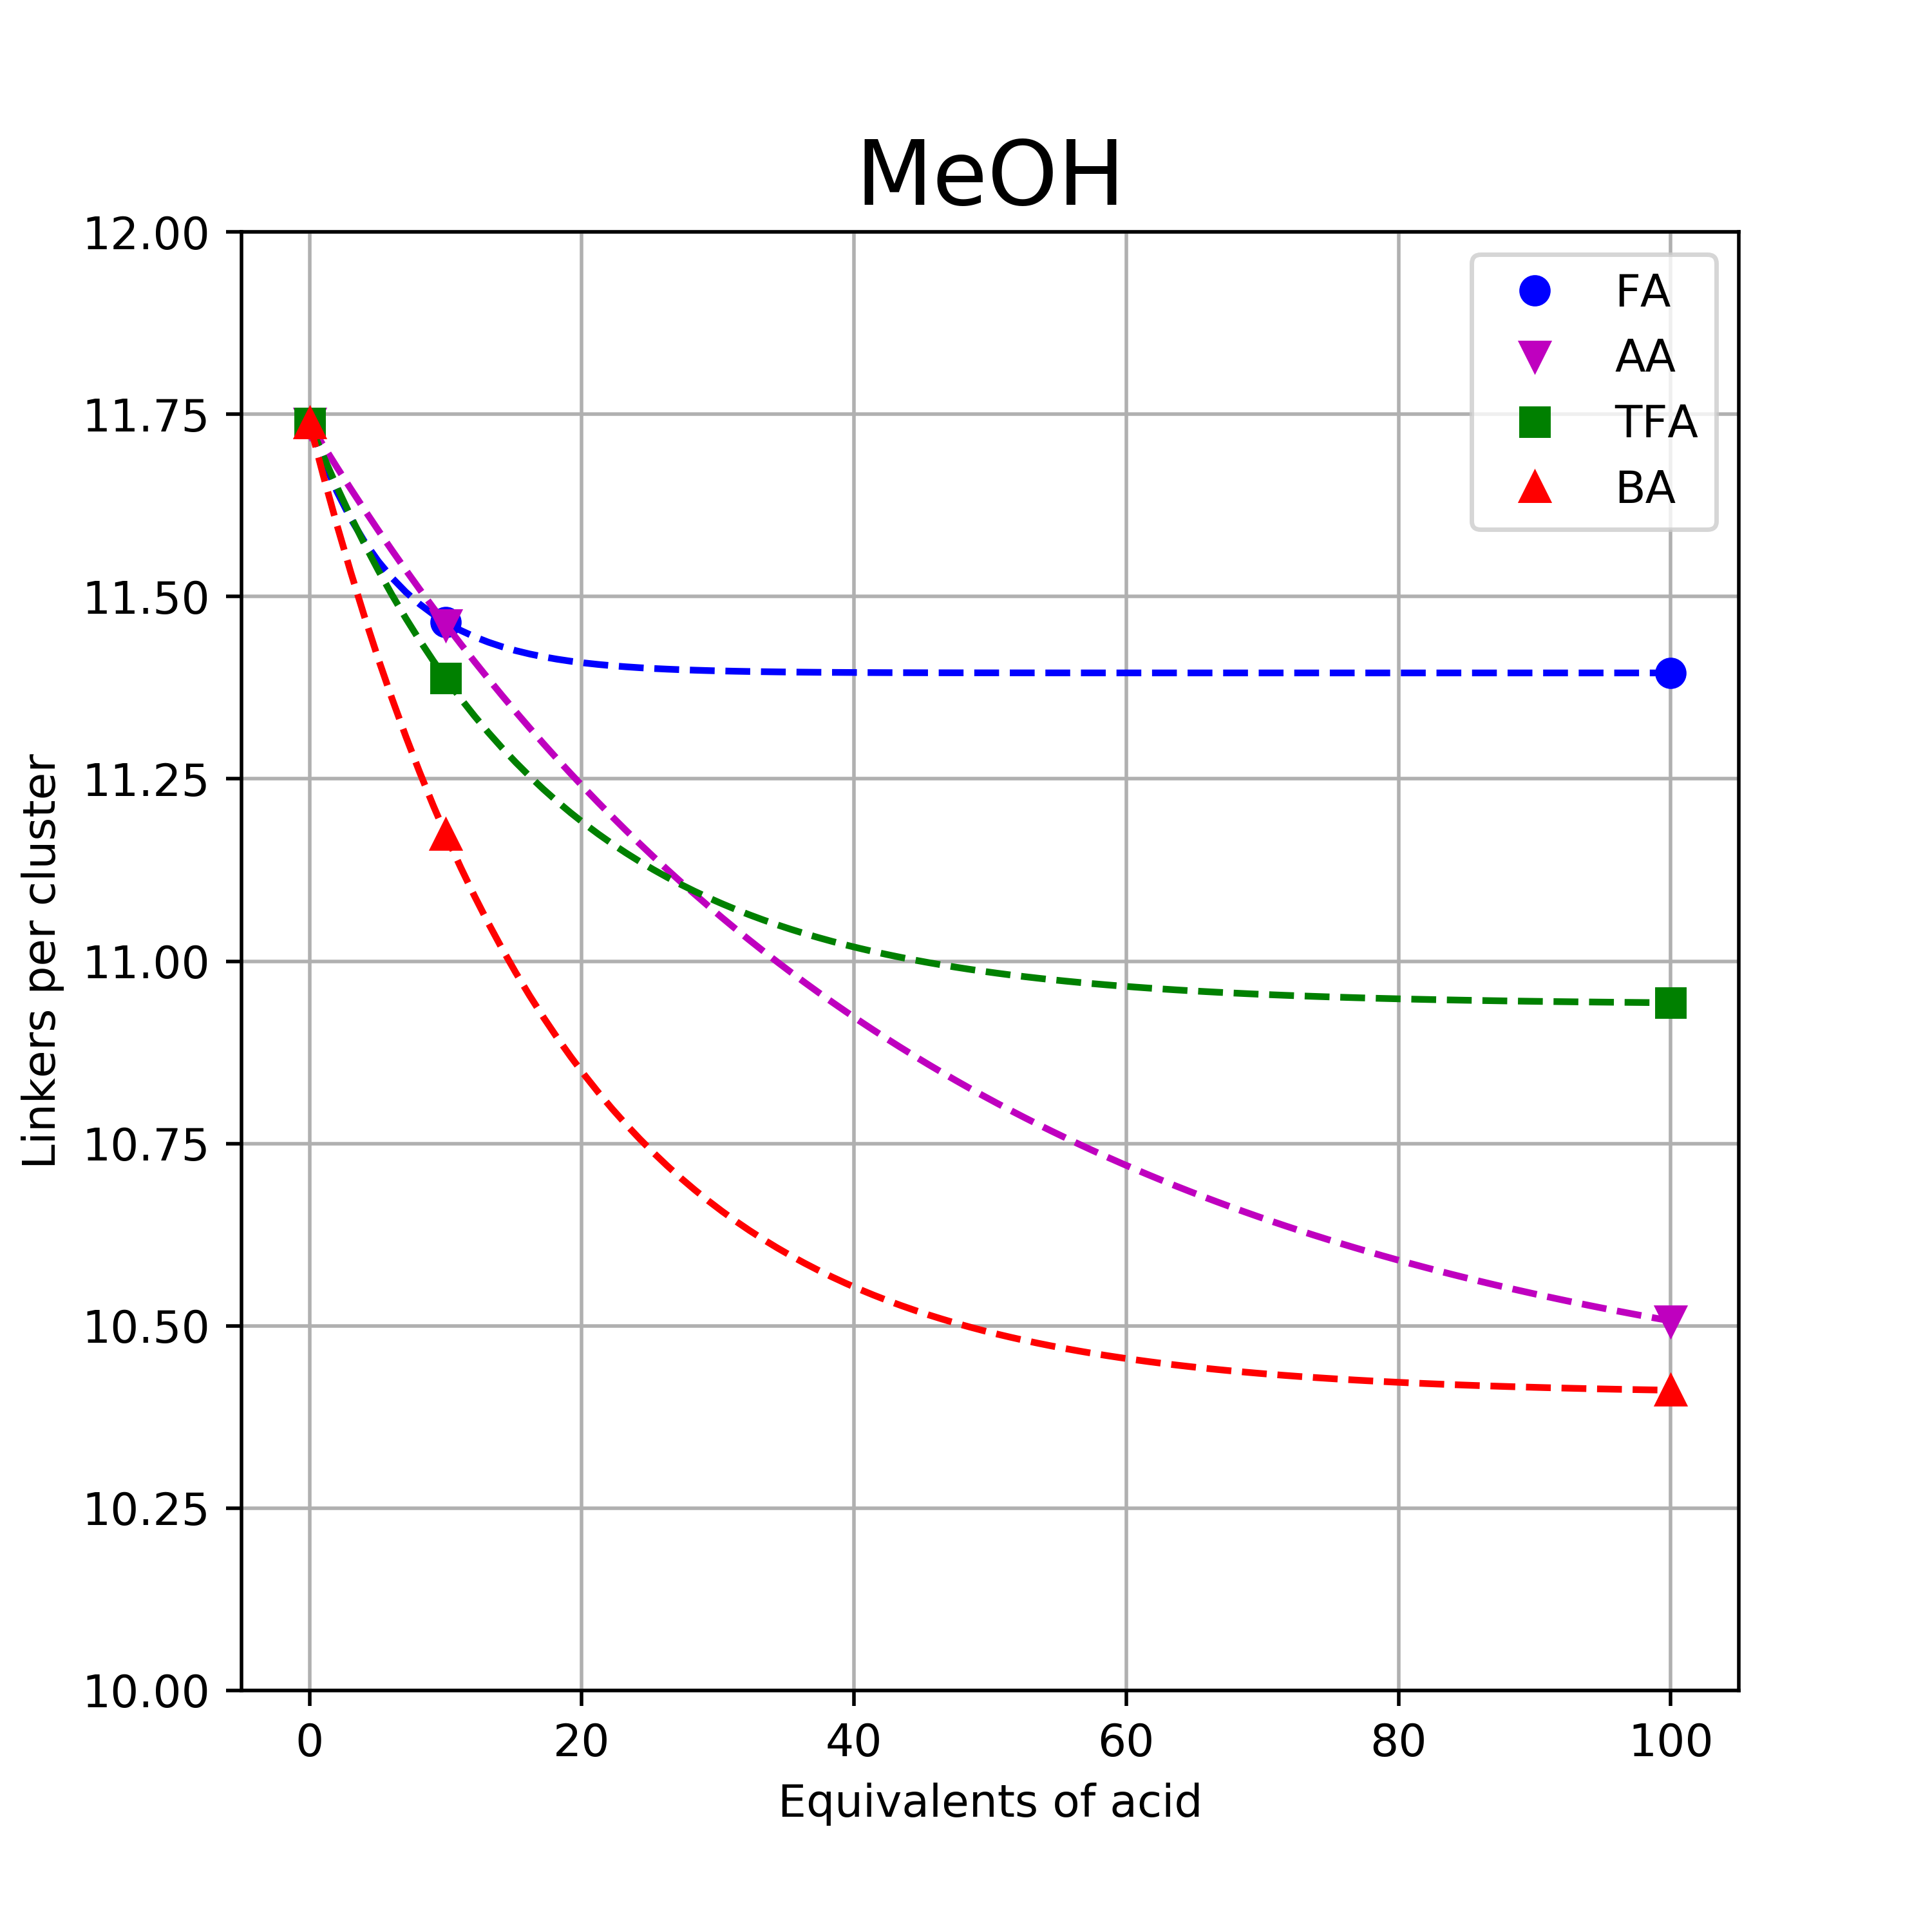
\includegraphics[width=\textwidth]{tga/MeOH-def-overview}%
        \label{def:fgr:tga-meoh-linkers}
    \end{subfigure}
    \begin{subfigure}{0.45\linewidth}
        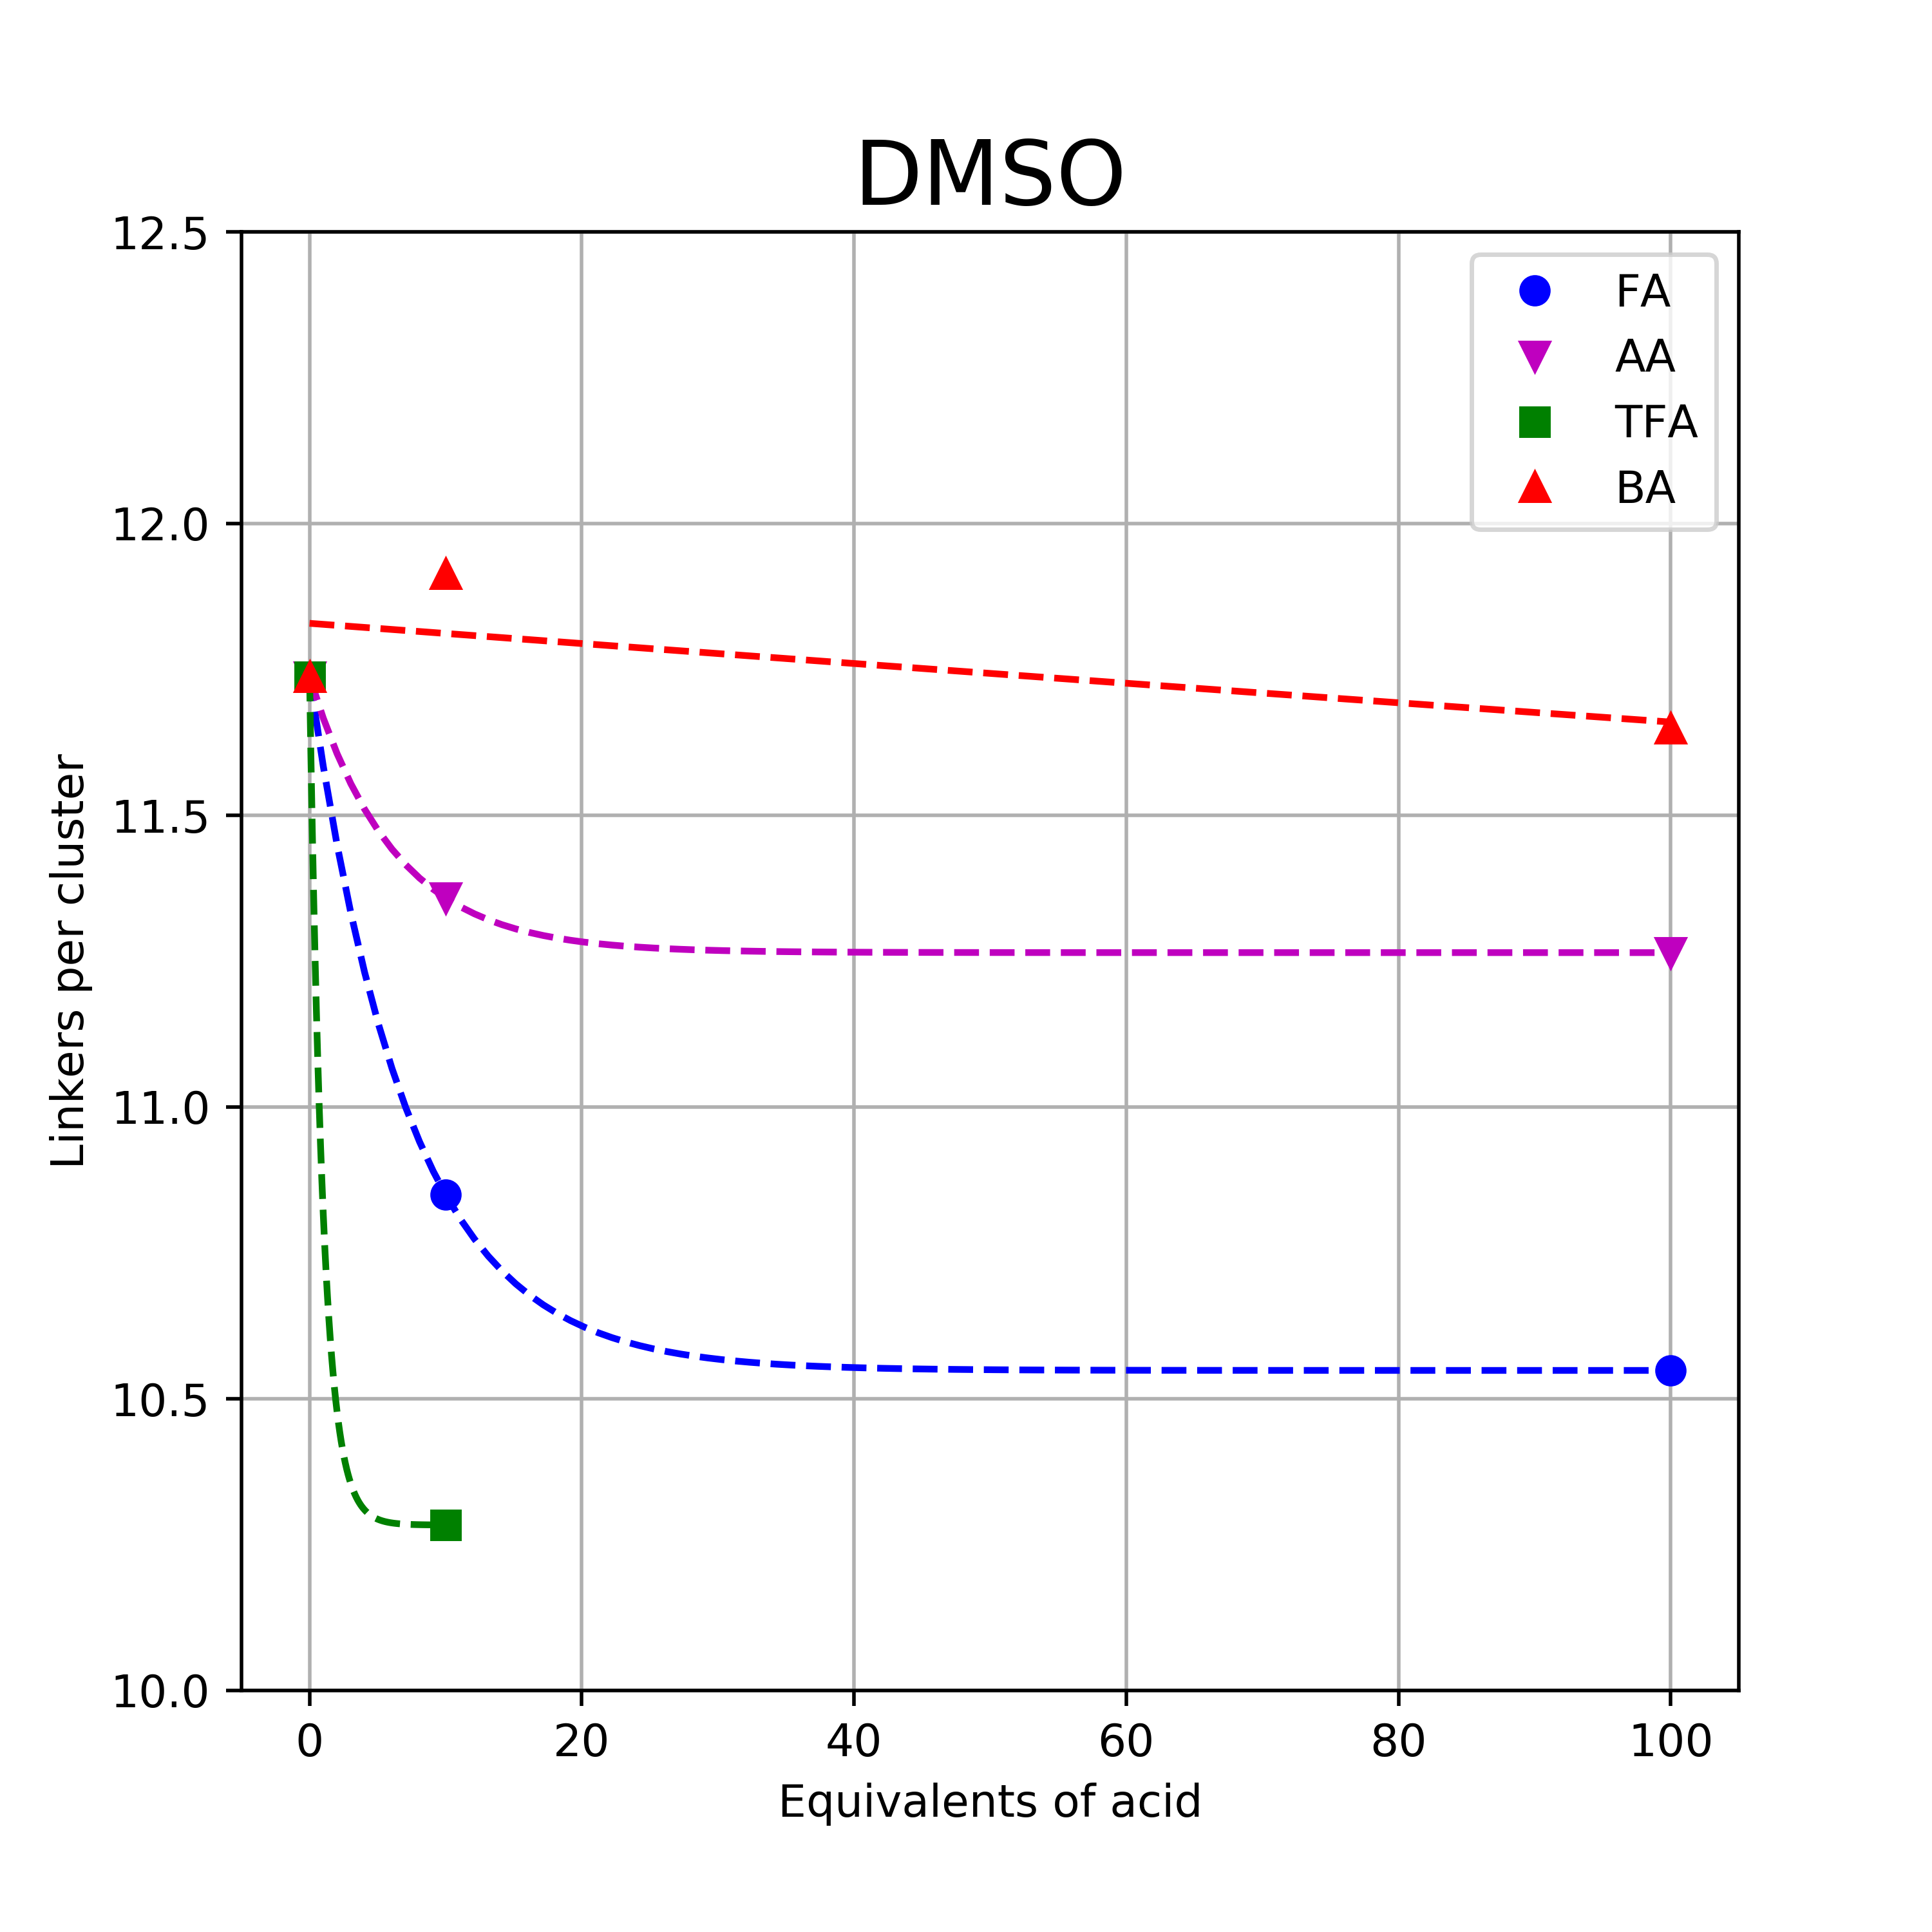
\includegraphics[width=\textwidth]{tga/DMSO-def-overview}%
        \label{def:fgr:tga-dmso-linkers}
    \end{subfigure}

    \caption{Calculated linker-to-node ratio from the TGA curve 
    normalized mass at \SI{420}{\degreeCelsius} for (a) DMF 
    (b) \ce{H2O}, (c) \ce{MeOH} and (d) DMSO leached samples.
    A ratio of 12 to 1 corresponds to a completely defect-free
    structure.}%
    \label{def:fgr:tga-defects}
    
\end{figure}


When DMF is used as a solvent, the resulting leached samples 
have a 

Since multiple concentrations of modulator were used only with 
DMF, inly a general trend is available.
% !TEX root = ../../main.tex

\subsection{Nitrogen sorption at 77K}

Isotherms have been recorded on samples activated at both
\SI{200}{\degreeCelsius} and \SI{320}{\degreeCelsius}.
It is important to note that, as seen from the TGA curves,
not all capping agents leave the structure when thermal treating
at a lower temperature. The moieties which are still coordinated
to the Zr cluster will likely influence the adsorption
behaviour. At a high temperature, the dehydroxilation of the 
metal center also occurs~\cite{valenzanoDisclosingComplexStructure2011},
which may also affect the interaction with physisorbed probes. 
Several example isotherms can be found in
\autoref{def:fgr:n2phys-dataset}, with the complete dataset
present in \autoref{appx:def}, \autoref{appx:def:n2phys}.

There are a few isotherm features which can be analysed to
assess the type of modifications introduced in the structure
and their preponderence.

\begin{itemize}
	\item The slope of the isotherm at low \(p/p_0\) is representative
	      of the first interactions with the pore surface, which can be
	      quantified using the initial Henry constant. It will be influenced
		  by any changes in pore environment such as CUS or functionalised
		  defect sites.
	\item Missing liker defects will lead to an increase of the
	      apparent surface area and perhaps to a more extensive
	      pore network.
	\item The pore size distribution and total pore volume give
	      indications on the presence of missing cluster defects and/or
	      of the formation of mesoporous voids within the structure.
	\item A steep step at high \(p/p_0\) is indicative of intercrystal
	      condensation and suggests particle aggregation due to lower average
	      crystal size.
\end{itemize}

\begin{figure}[htbp]
	\centering

	\begin{subfigure}{0.45\linewidth}
		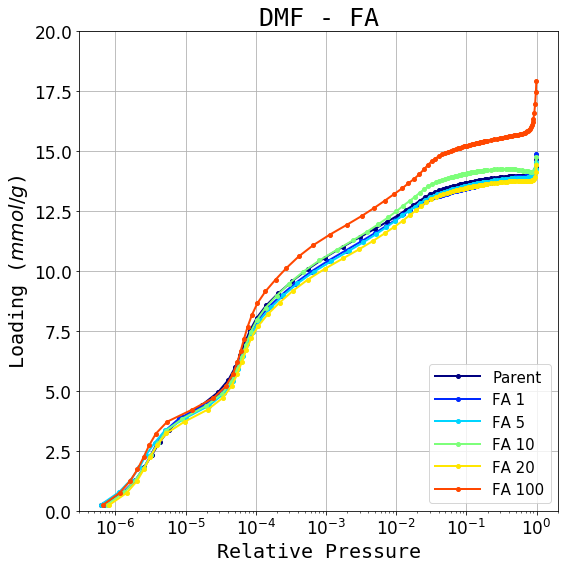
\includegraphics[width=\textwidth]{n2phys/dmf-fa}%
		\caption{}%
		\label{def:fgr:n2phys-dmf-fa}
	\end{subfigure}
	\begin{subfigure}{0.45\linewidth}
		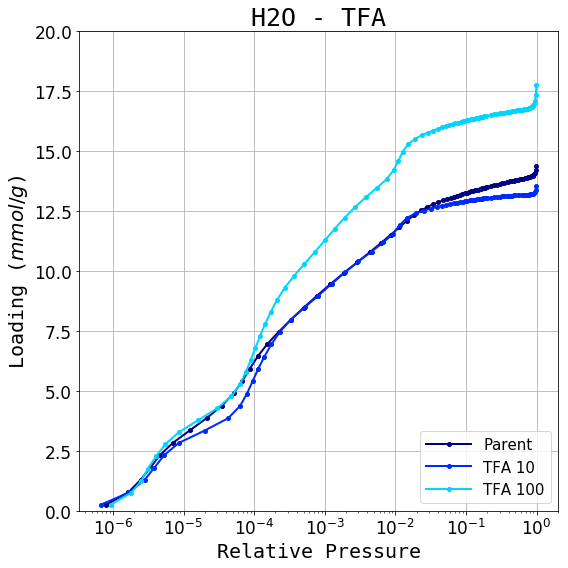
\includegraphics[width=\textwidth]{n2phys/h2o-tfa}%
		\caption{}%
		\label{def:fgr:n2phys-h2o-tfa}
	\end{subfigure}

	\begin{subfigure}{0.45\linewidth}
		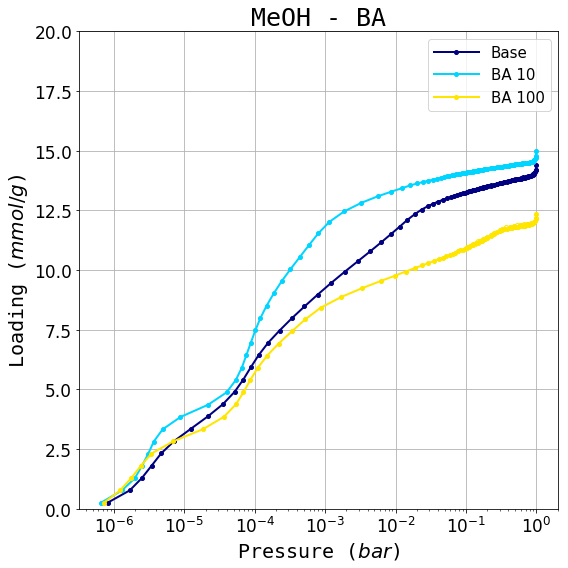
\includegraphics[width=\textwidth]{n2phys/meoh-ba}%
		\caption{}%
		\label{def:fgr:n2phys-meoh-ba}
	\end{subfigure}
	\begin{subfigure}{0.45\linewidth}
		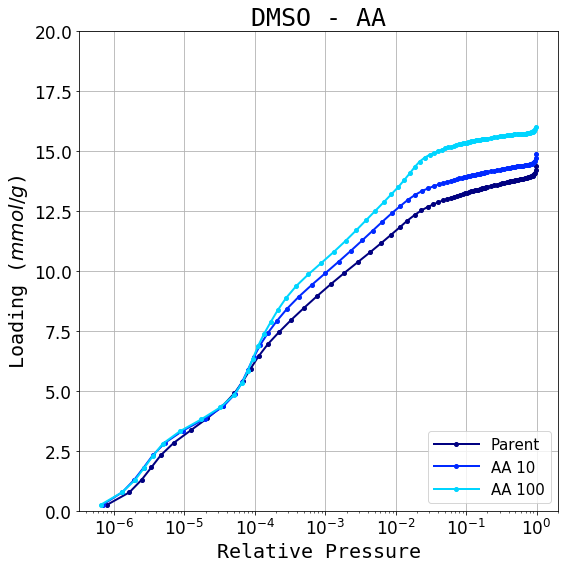
\includegraphics[width=\textwidth]{n2phys/dmso-aa}%
		\caption{}%
		\label{def:fgr:n2phys-dmso-aa}
	\end{subfigure}

	\caption{A selection of nitrogen sorption isotherms as measured on the
		leached samples at \SI{200}{\degreeCelsius}: (a) formic acid in DMF,
		(b) trifluoroacetic acid in water, (c) benzoic acid
		in methanol and (d) acetic acid
        in DMSO. The curve for the parent material is in dark blue.
        The x axis is logarithmic for clarity of low pressure 
        points.}%
	\label{def:fgr:n2phys-dataset}
\end{figure}

It is immediately apparent that the leaching process had an influence 
on the adsorption characteristics of UiO-66. Isotherms of acid treated
samples diverge from the parent material, often at different pressures.
In general, the total molar capacity at full loading is seen to increase,
a telltale sign of an increase in pore volume through defect generation.
On the other hand, other particularities exist, such as the benzoic acid
samples in methanol and DMSO where the low and high
concentration has opposite effect on the total loading. Predictors 
of defects and trends will be analysed in the following section.

\subsection{Room temperature gas adsorption and microcalorimetry}

As previously shown, combining microcalorimetry with adsorption manometry
can give an insight into the energetics of the
adsorption process by directly measuring differential heat.
Even though the different contributions to the overall enthalpy curve
cannot be decoupled from the individual sources, such as guest-host
interactions or fluid-fluid interactions, it can be successfully
applied to observing the effect of a process or treatment such as shaping
on the properties of a MOF.

Eight probe gasses have been chosen for adsorption at \SI{303}{\kelvin}:
\ce{N2}, \ce{CO}, \ce{CO2}, \ce{CH4}, \ce{C2H6}, \ce{C3H6},
\ce{C3H8} and \ce{C4H10}.
The range of adsorbates chosen allows different effects to be investigated.
The adsorption of saturated hydrocarbons with an increasing
carbon number (C1-C4) can be
assumed to be driven strictly by Van-der-Waals forces,
due to the shielding effects of the hydrogen atoms.
Differences in the maximum uptakes of these gasses will point to
loss of porosity or crystalinity. A capacity loss with
an increasing carbon number will point to size exclusion effects
induced by the binder, such as particle coating, pore filling or
pore obstruction.
The other probes have been chosen for their properties which can
shine light on other specific interaction types
present during the adsorption.
Carbon monoxide is a slightly dipolar molecule which has the
ability to act as an with other charges in the pores.
It also can highlight CUS (coordinatively unsaturated sites)
generated through defects, reduction or open metal sites due to its
propensity for \( \pi \) backbonding coordination.
This electron transfer process can also result in complexation with molecular
orbitals in systems with \( \pi \) bonds such as alkenes and alkynes.
Propylene is used as an unsaturated hydrocarbon probe gas for this purpose.
Carbon dioxide is a highly quadrupolar molecule which will be
strongly adsorbed in polar pore environments. Changes in the adsorption
behaviour of \ce{CO2} will shed light on such surface changes and
can even be used as a predictor
of hydrophobicity~\cite{chanutScreeningEffectWater2017}.
Finally, \ce{N2} is a staple adsorbent for material characterisation
when used at \SI{77}{\kelvin}. The molecule is a slight quadrupole
and has also been shown to chelate to some transitional metals in
an analogue fashion to \ce{CO}.

To eliminate the influence of kinetic and diffusion effects on the experiments,
care has been taken to allow time for complete equilibration of both pressure
and calorimeter signal.
The complete dataset of adsorption isotherms, in the basis of both mass
and volume can be found in \autoref{appx:shaping}.

After collecting the combined isotherm and enthalpy data, three
indicators have been chosen to best represent the effects of shaping:
initial enthalpy of adsorption, initial Henry constant and maximum capacity.
These numeric performance indicators have been calculated using the
available functionality in pyGAPS.

The initial enthalpy of adsorption extrapolated at zero coverage is
a measure of the interaction with highest energetic sites on the MOF
surface. Conversely, the initial Henry constant (\(K_{Hi}\)), here obtained through 
fitting the virial adsorption model through the method in
\autoref{pyg:models:virial},
is also an indication of adsorption in the pores before any
layering or adsorbate-adsorbate interaction comes into effect.
The last indicator, maximum capacity, was taken as the loading attained when
the isotherm reached a plateau. In the case of probes where the plateau
was outside the range of pressure of the instrumentation (>\SI{50}{\bar}),
the loading at the highest available pressure was considered as a
suitable approximation.
The three key performance indicators (KPIs) have then been compared side by
side on both the powder and shaped samples.

% !TEX root = ../../main.tex

\subsubsection{UiO-66(Zr)}

A visual inspection of the enthalpy curves on as-synthesised UiO-66(Zr)
shows it to be relatively homogenous, with flat
profiles being common. This is typical of this \gls{MOF}, which has
a pore environment without high energy adsorption 
sites~\cite{wiersumEvaluationUiO66GasBased2011}.
Both \ce{CO2} and \ce{CO} show a higher enthalpy of adsorption
at low loadings, as seen in \autoref{shaping:fig:uio66isotherms},
which is likely due to their quadrupole and dipole interaction,
respectively.

\begin{figure}[p!]
	\centering
	\begin{subfigure}{\linewidth}
		\parbox[c]{0.1\linewidth}{\caption{}%
			\label{shaping:fig:analysisuio66henry}}%
		\parbox[b]{0.8\linewidth}{%
			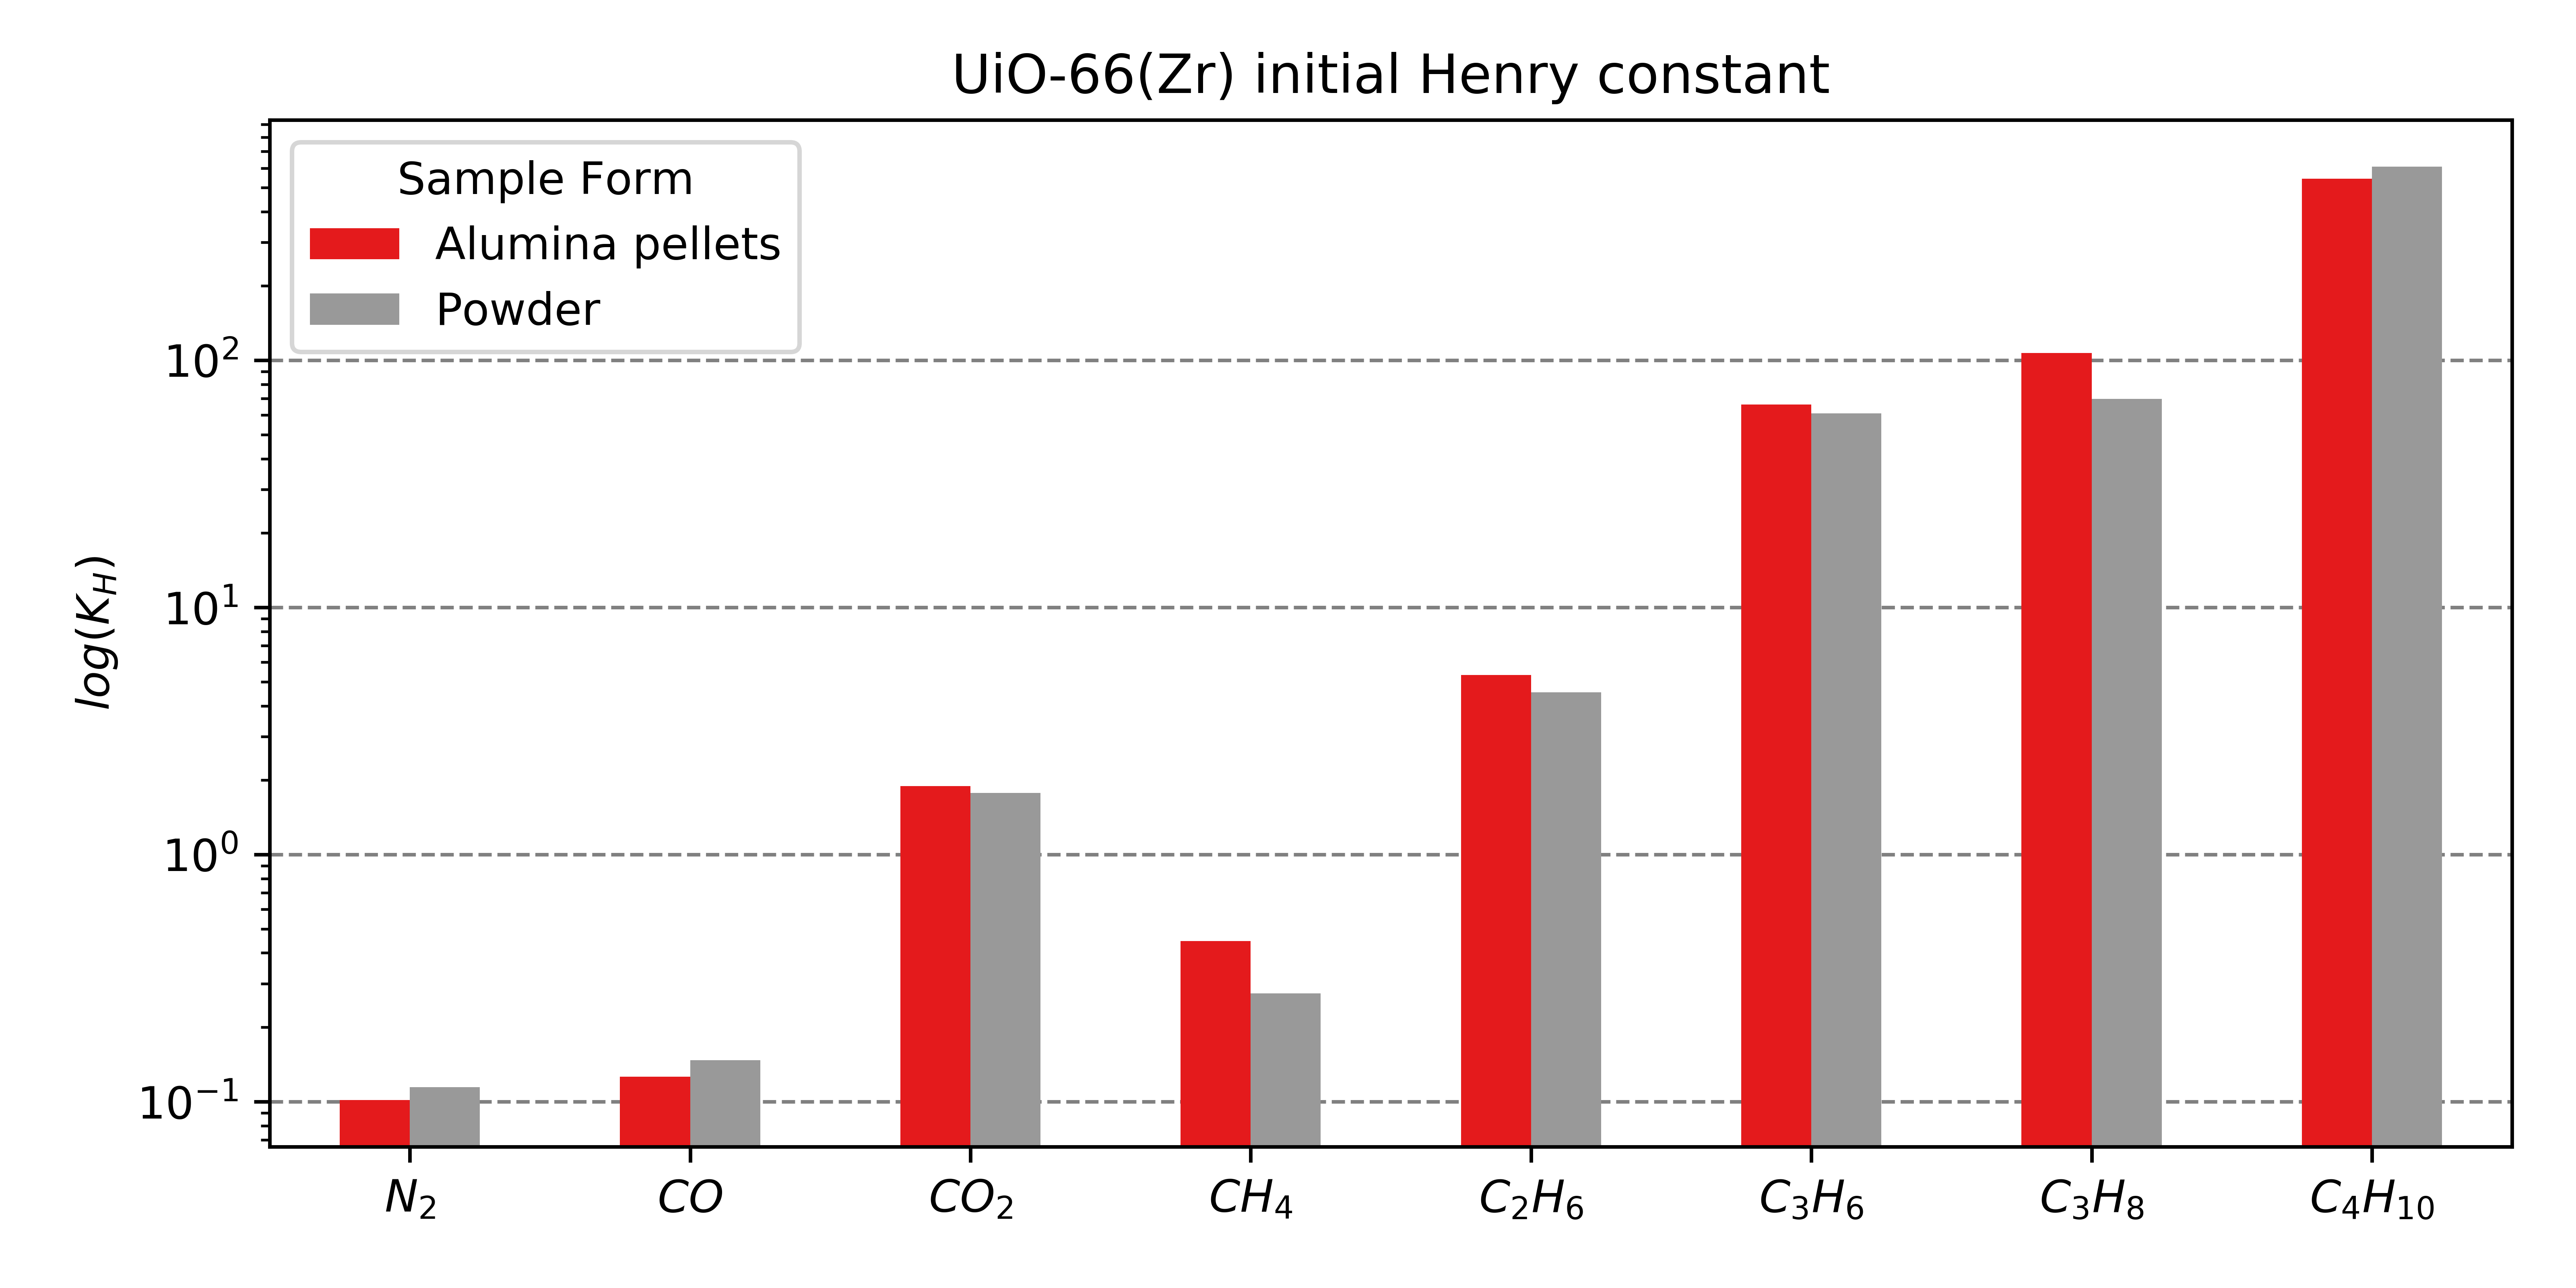
\includegraphics[width=\linewidth]{UiO-66(Zr)-henry-distribution}%
		}%
	\end{subfigure}%

	\begin{subfigure}{\linewidth}
		\parbox[c]{0.1\linewidth}{\caption{}%
			\label{shaping:fig:analysisuio66enth}}%
		\parbox[b]{0.8\linewidth}{%
			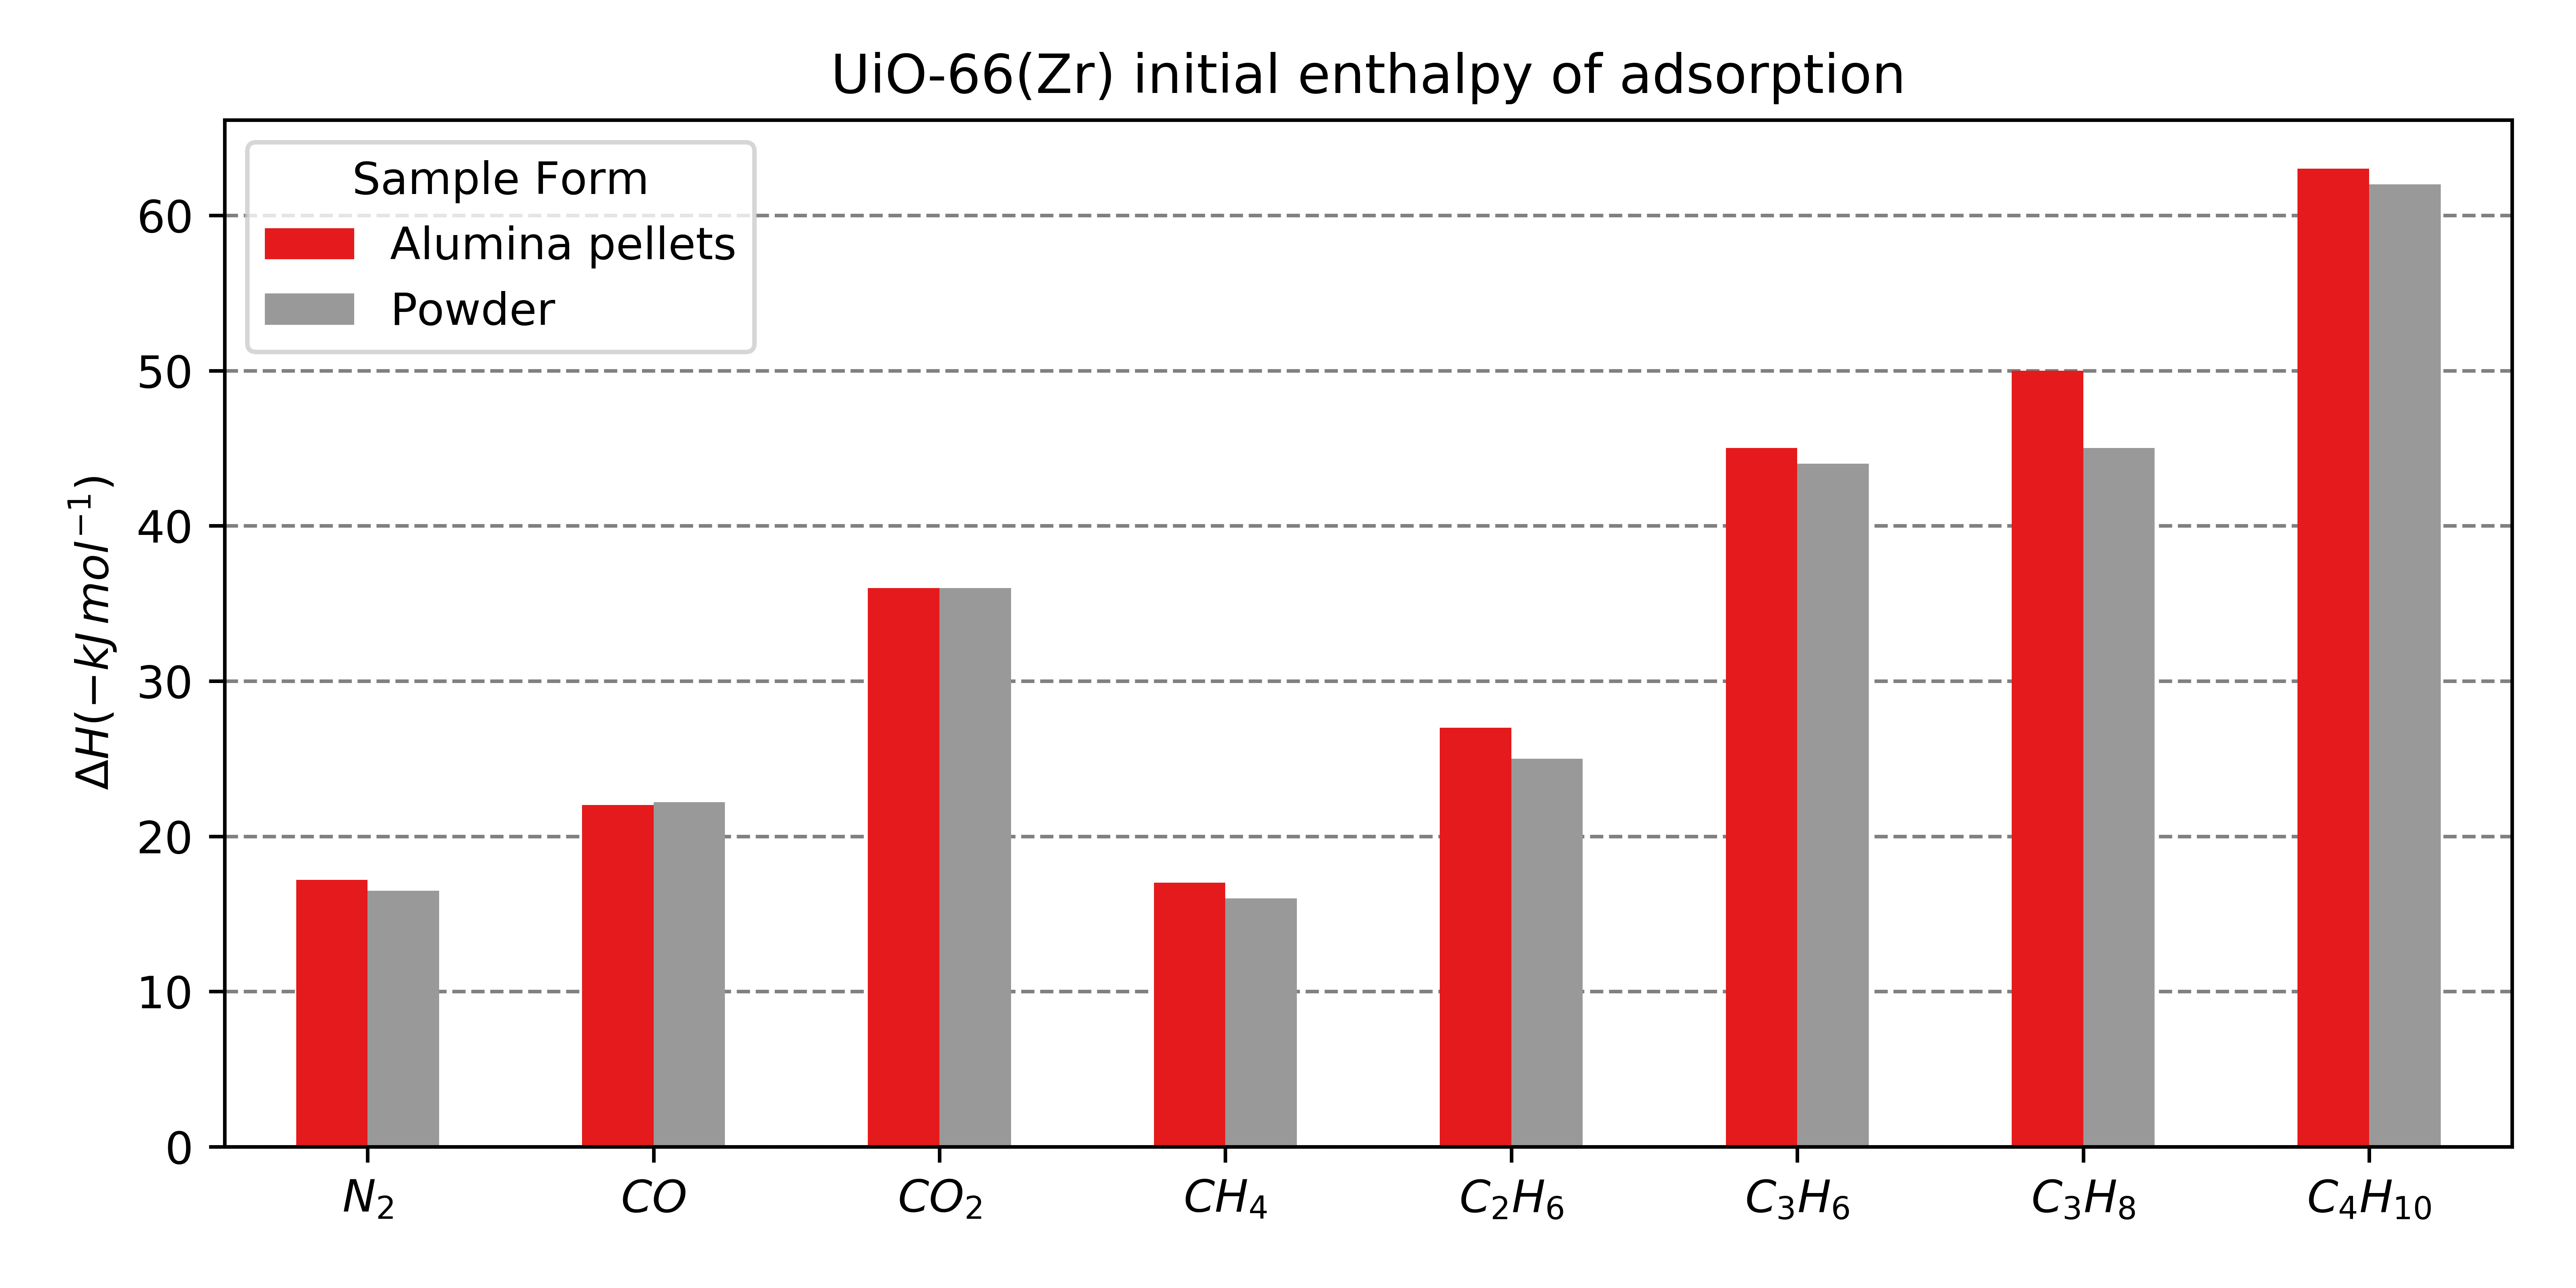
\includegraphics[width=\linewidth]{UiO-66(Zr)-enthalpy-distribution}%
		}%
	\end{subfigure}%

	\begin{subfigure}{\linewidth}
		\parbox[c]{0.1\linewidth}{\caption{}%
			\label{shaping:fig:analysisuio66basis}}%
		\parbox[b]{0.8\linewidth}{%
			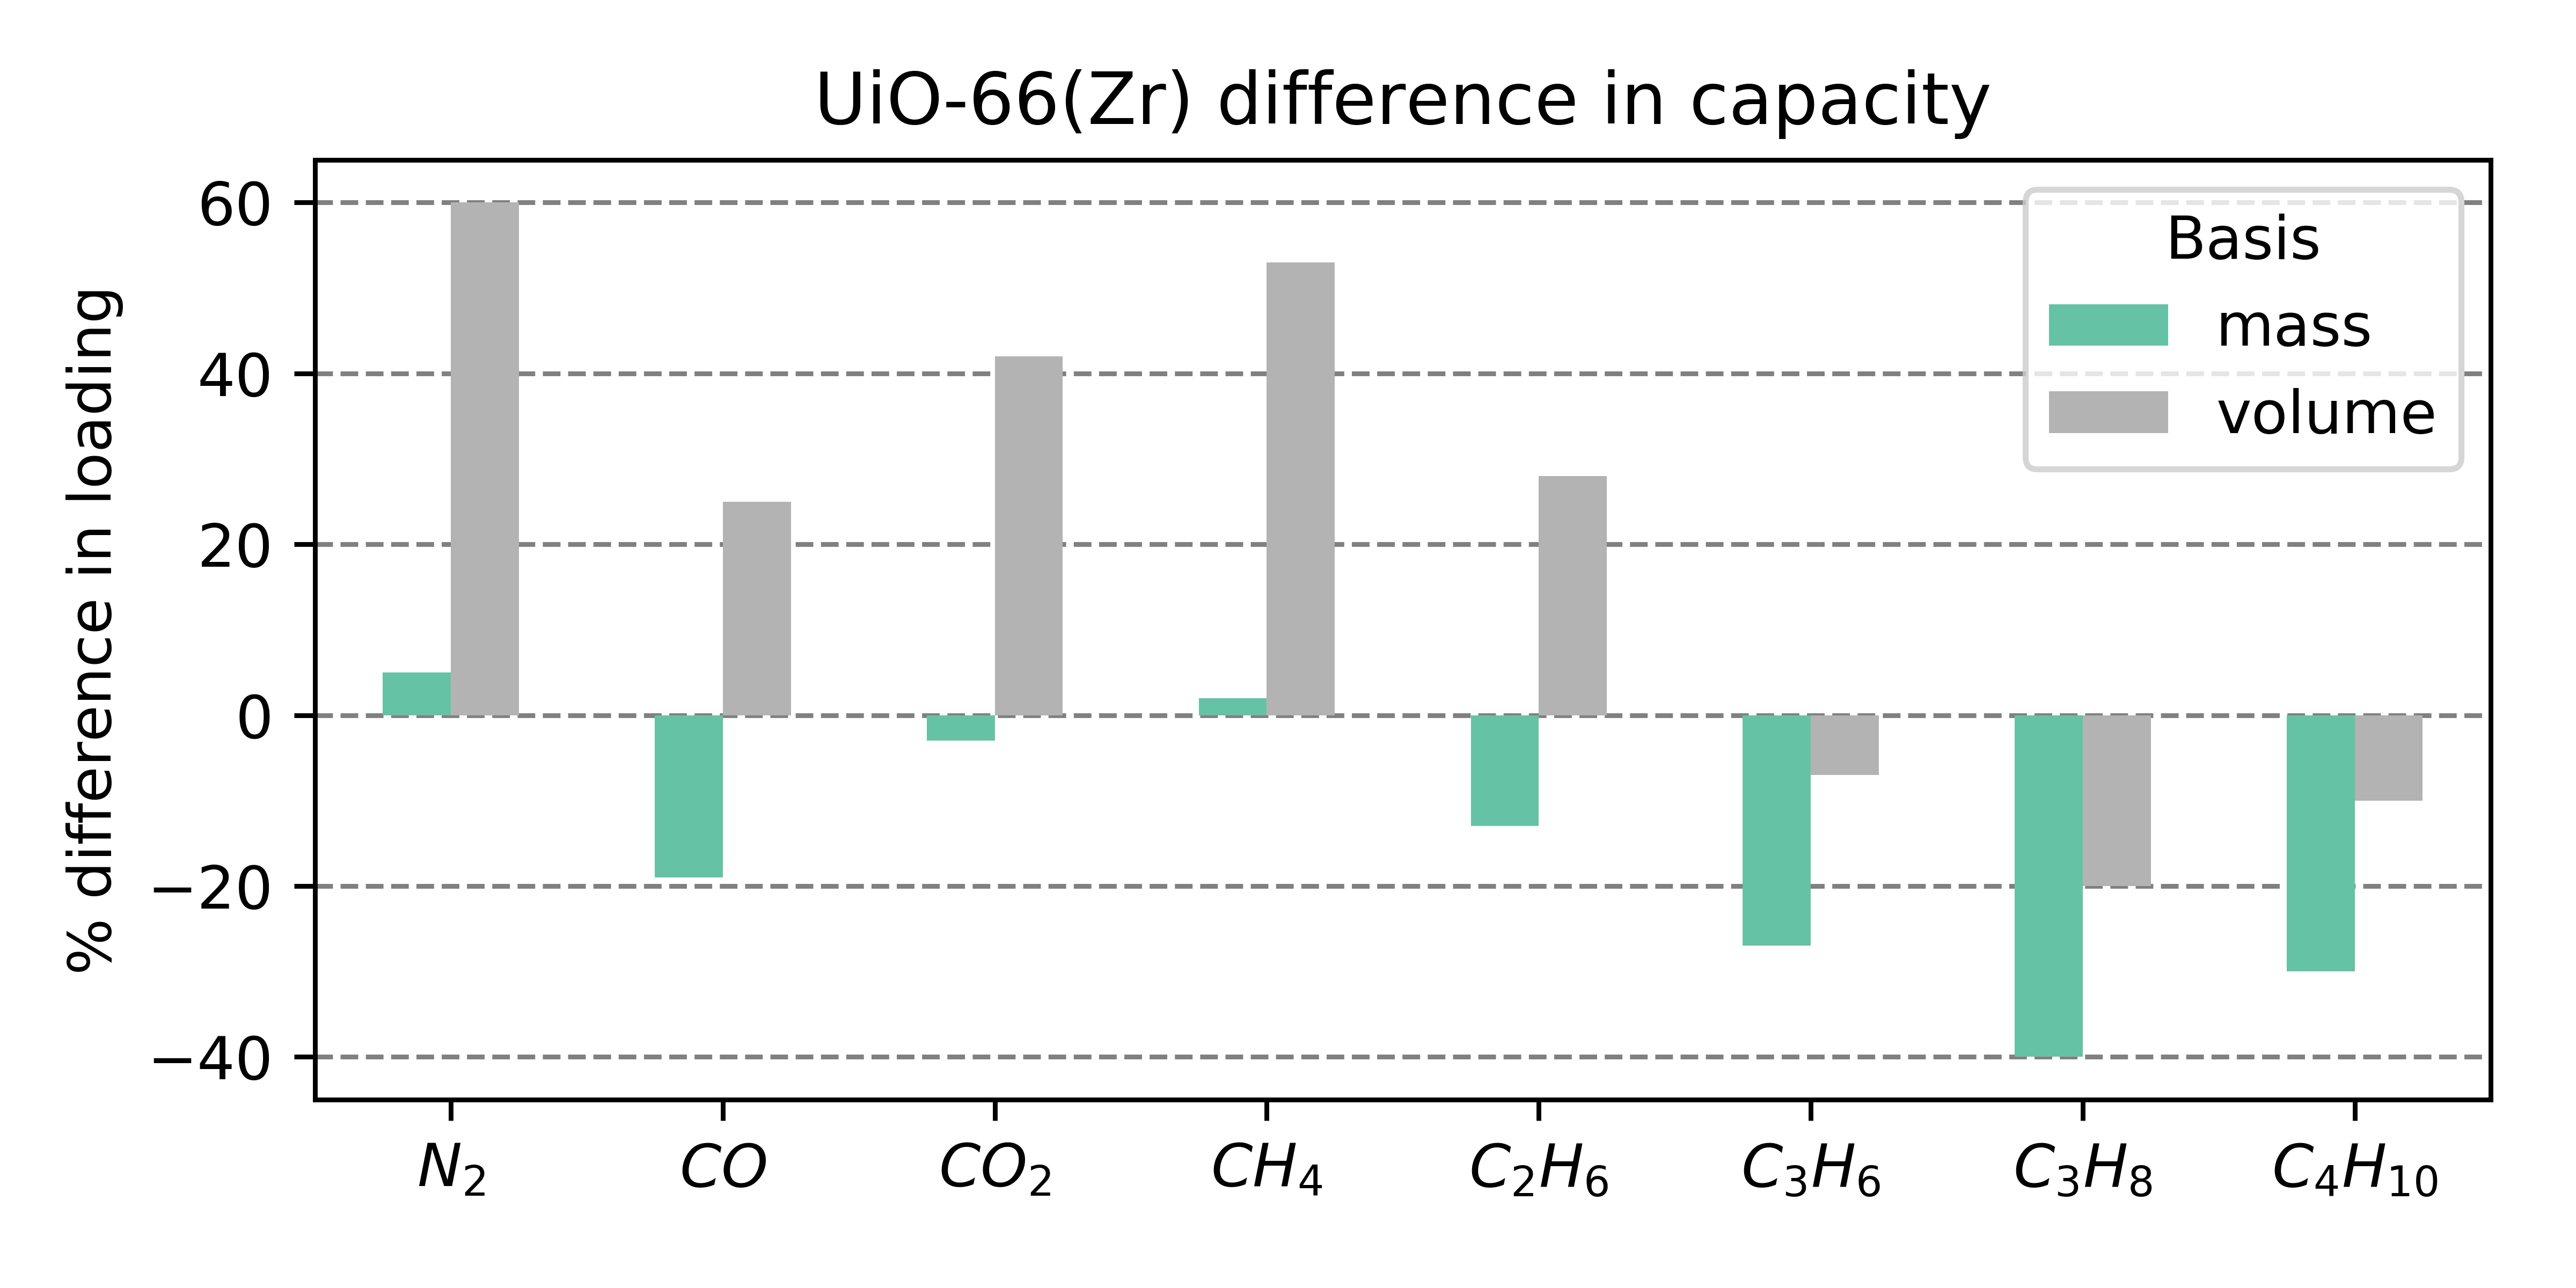
\includegraphics[width=\linewidth]{UiO-66(Zr)-mass-volume}%
		}%
	\end{subfigure}%

	\caption{\glspl{KPI} extracted from the UiO-66(Zr) adsorption dataset with
		(a) logarithmic initial Henry constant (b) initial enthalpy of
        adsorption and (c) change in adsorption maximum capacity from 
        the powder to the alumina shaped version on a mass and volume 
        basis in red and grey respectively}%
	\label{shaping:fig:analysisuio66}
\end{figure}

\begin{figure}[htb]
	\centering
	\begin{subfigure}{0.45\textwidth}
		\includegraphics[width=\linewidth]{calo/UiO-66(Zr)/co2-mass-basis-iso}
		\caption{\ce{CO2} adsorption isotherms}%
		\label{shaping:fig:uio66co2ads}
	\end{subfigure}%
	\begin{subfigure}{0.45\textwidth}
		\includegraphics[width=\linewidth]{calo/UiO-66(Zr)/co-mass-basis-iso}
		\caption{\ce{CO} adsorption isotherms}%
		\label{shaping:fig:uio66coads}
	\end{subfigure}%
	\caption{Selected isotherms from the UiO-66(Zr) dataset}%
	\label{shaping:fig:uio66isotherms}
\end{figure}

The \gls{KPI} graphs in \autoref{shaping:fig:analysisuio66} show very
similar values for both initial Henry's constant and initial
enthalpy of adsorption. It is therefore apparent that the shaping process
did not change the interaction of the adsorbate with the \gls{MOF} surface.

The maximum capacity graphs show a more interesting trend.
When using small adsorbates such as \ce{N2}, \ce{CO2} and \ce{CH4},
the shaped samples have a similar performance on a mass basis and,
due to the densification process, better capacities on a volume
basis. Starting with ethane, the maximum capacity difference starts
to increase, with lower performance as molecule size increases.
On hydrocarbons with a carbon number of 3 and 4, both mass basis and
volume basis capacity are decreased compared to the original powder.
This size exclusion effect could be explained by the coating of
crystal surfaces and pore entrances with the alumina binder.

It could also be argued that instead of size exclusion, the effect is due to
an overall decrease in pore volume, and that the isotherms of the
low molecular weight gases will diverge at higher pressures
as the pores are filled. A counterargument for this hypothesis is that
in the case of \ce{CO2}, the plateau is reached with no differences
between the powder and the pellet as seen
in \autoref{shaping:fig:uio66co2ads}.

Carbon monoxide is an apparent outlier to this trend, with a
decreased maximum capacity and a small molecular size.
However, when observing the isotherms directly
(\autoref{shaping:fig:uio66coads}) it is obvious that the effect is
likely to be due to experimental errors, considering
the low amount adsorbed and the good overlap in the enthalpy
curves.

Overall, the shaping performance of UiO-66(Zr) is
reasonable, as long as only small adsorbates are used.

% !TEX root = ../../main.tex

\subsubsection{MIL-100(Fe)}

\begin{figure}[p]
	\centering
	\begin{subfigure}{\linewidth}
		\parbox[c]{0.1\linewidth}{\caption{}%
			\label{shaping:fig:analysismil100henry}}%
		\parbox[b]{0.8\linewidth}{%
			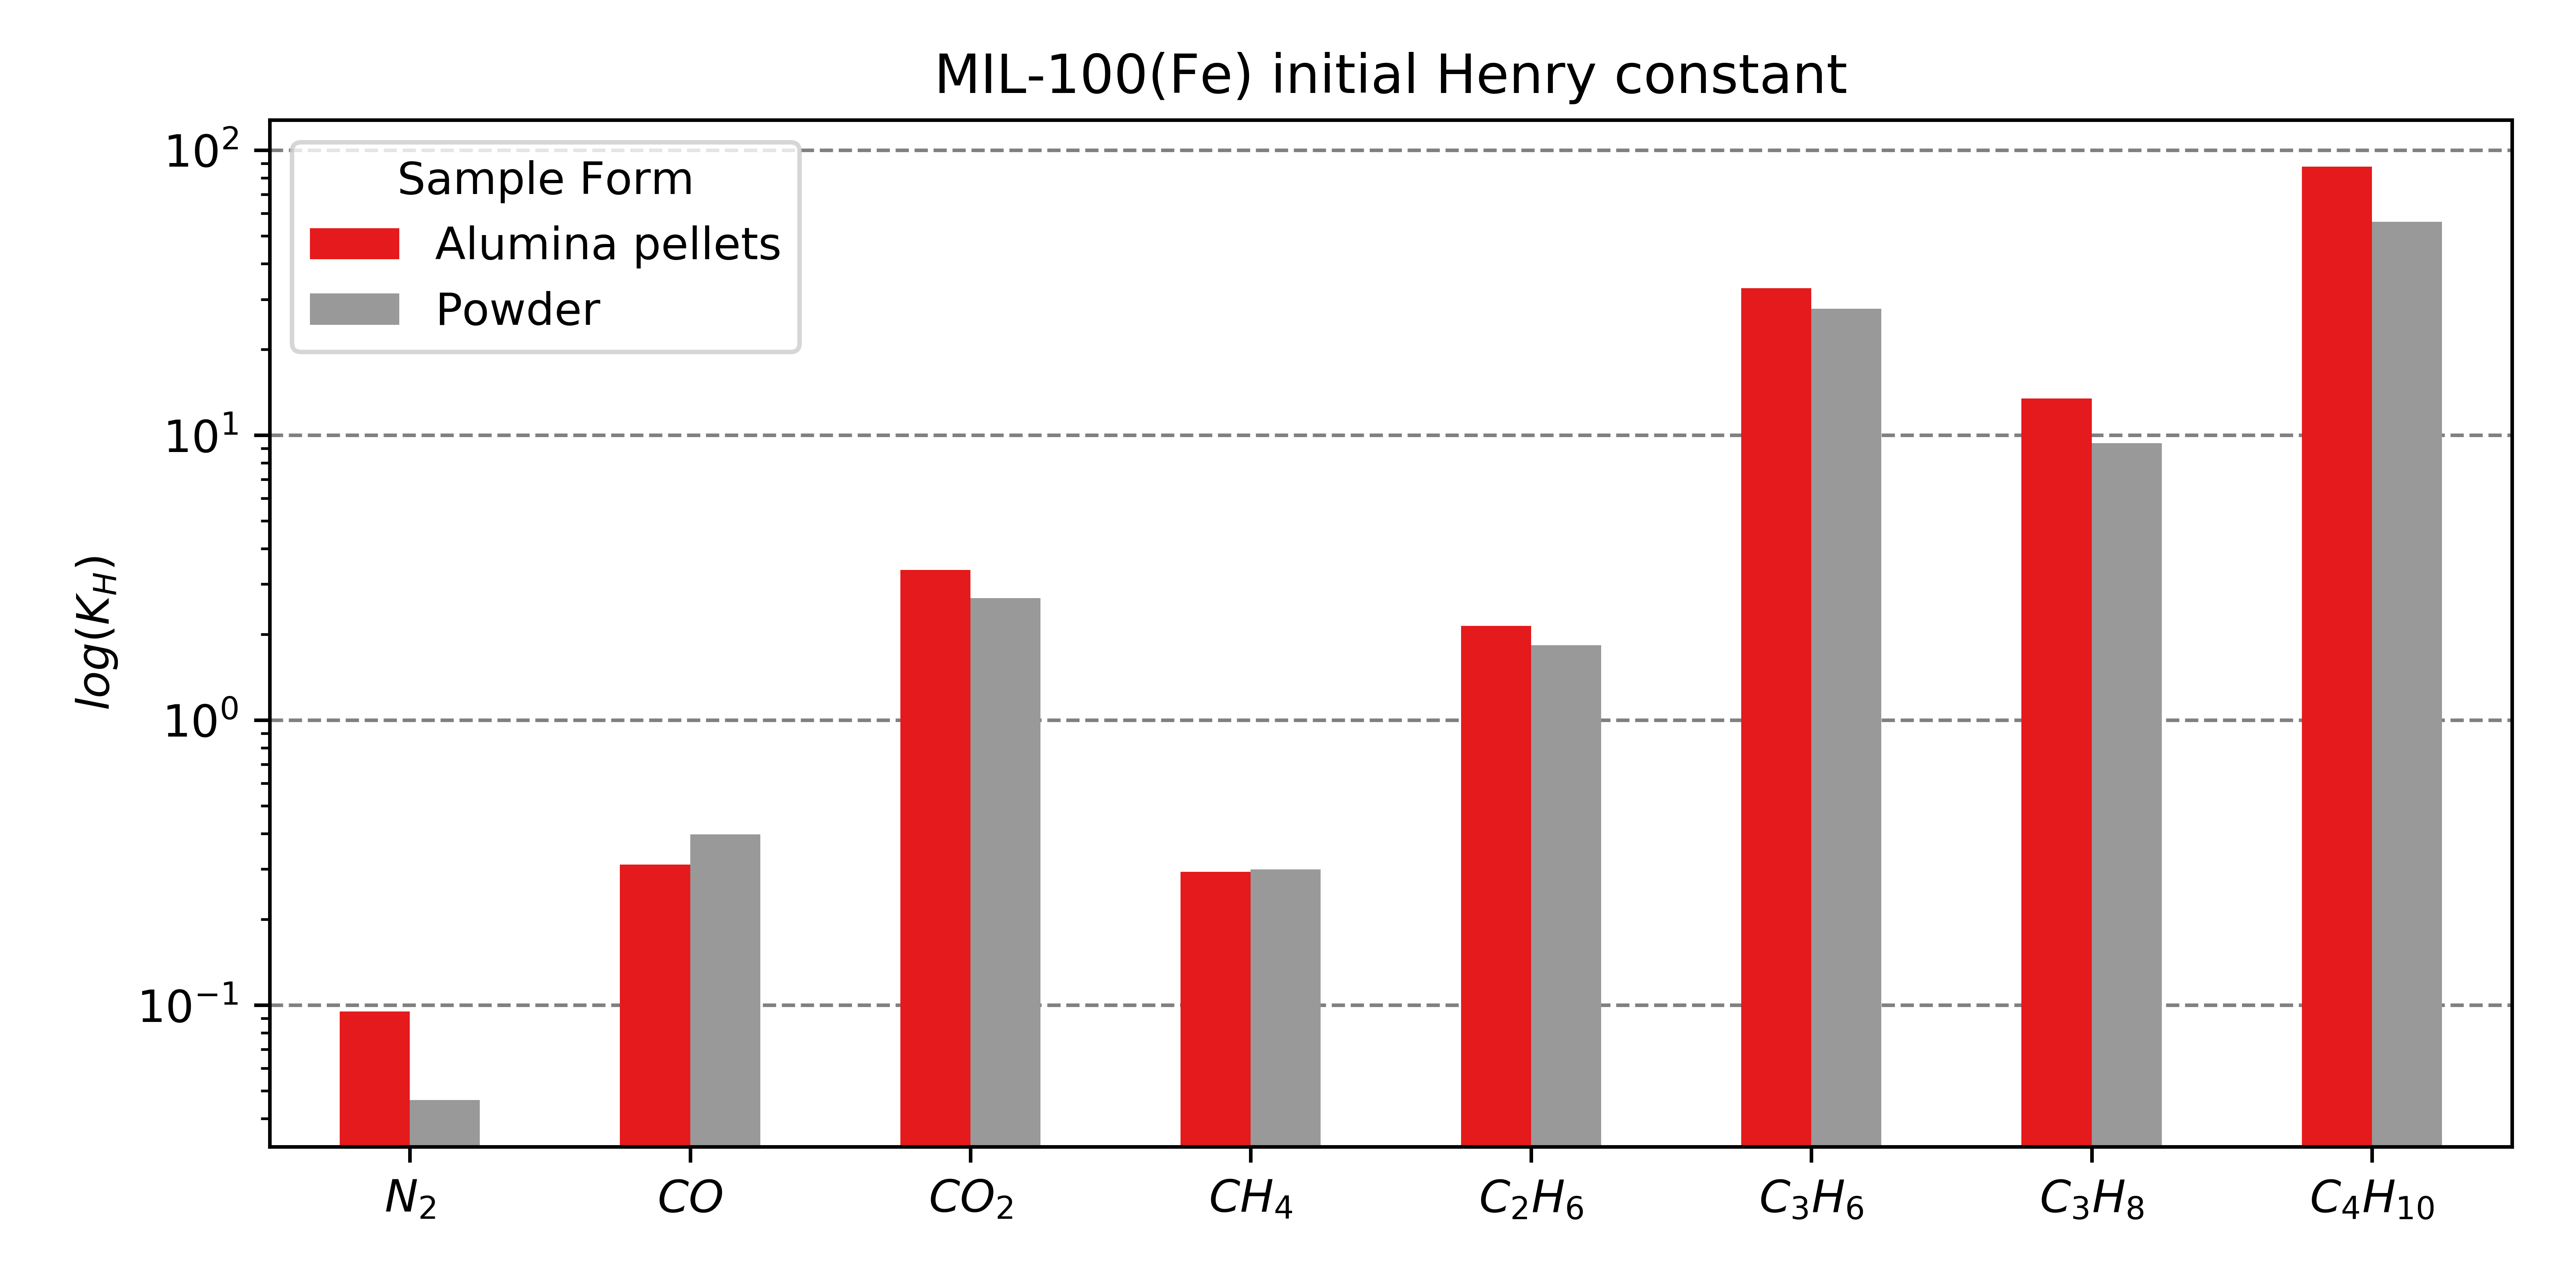
\includegraphics[width=\linewidth]{MIL-100(Fe)-henry-distribution}%
		}%
	\end{subfigure}%

	\begin{subfigure}{\linewidth}
		\parbox[c]{0.1\linewidth}{\caption{}%
			\label{shaping:fig:analysismil100enth}}%
		\parbox[b]{0.8\linewidth}{%
			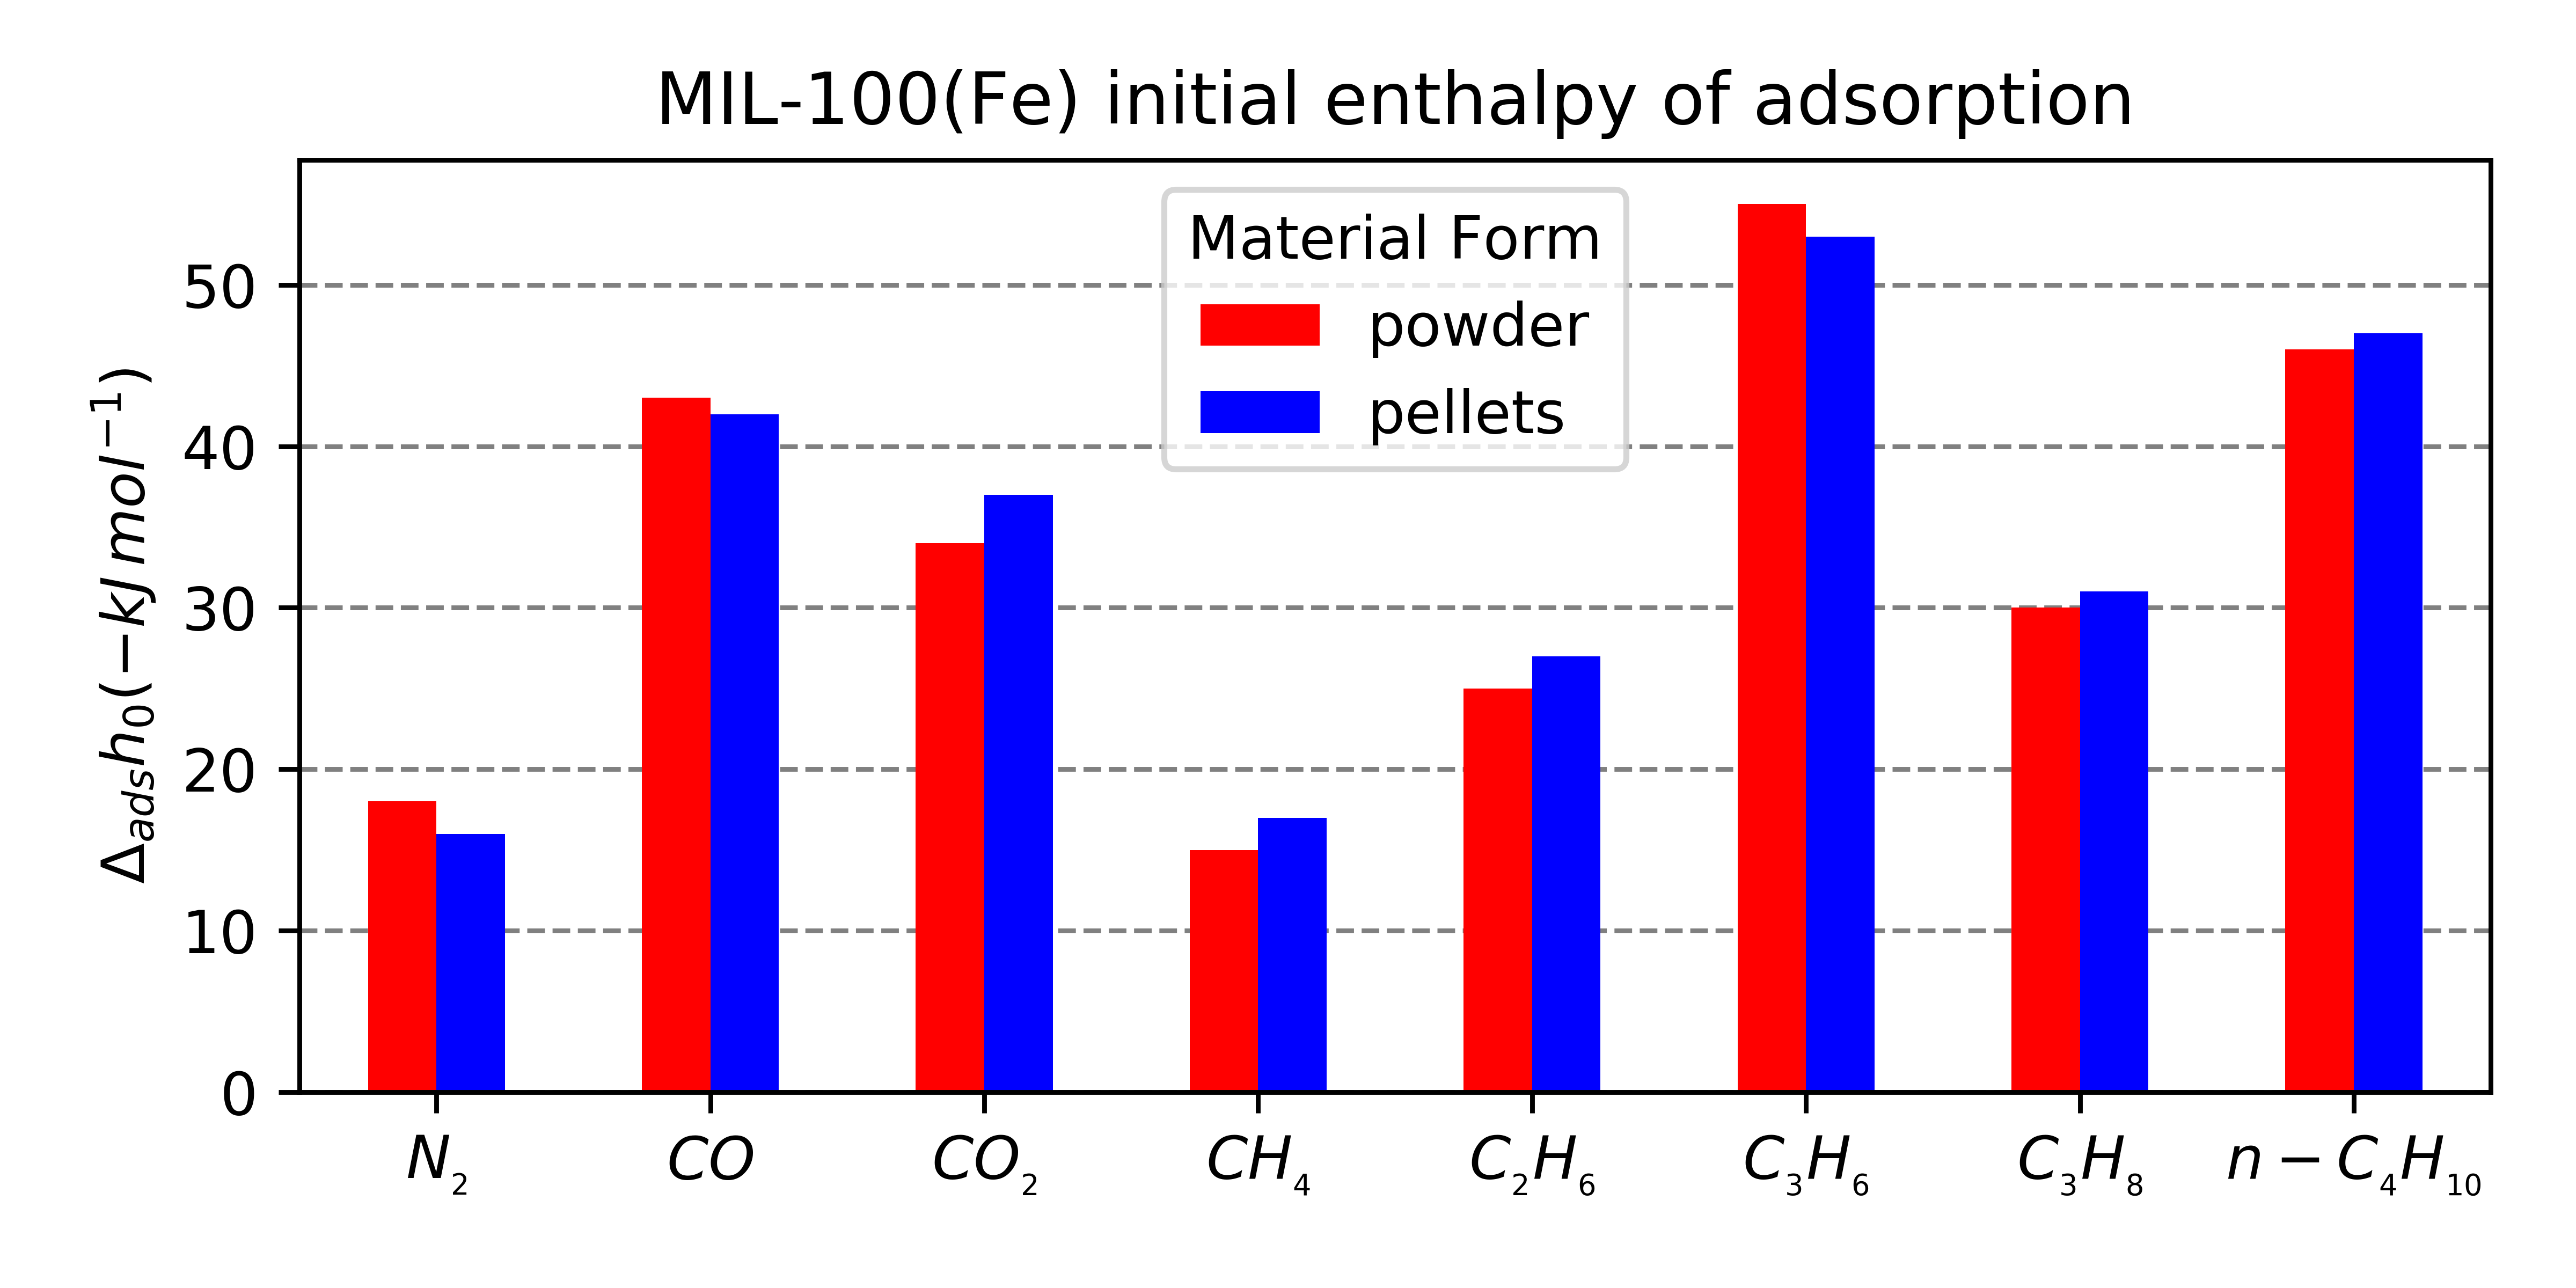
\includegraphics[width=\linewidth]{MIL-100(Fe)-enthalpy-distribution}%
		}%
	\end{subfigure}%

	\begin{subfigure}{\linewidth}
		\parbox[c]{0.1\linewidth}{\caption{}%
			\label{shaping:fig:analysismil100basis}}%
		\parbox[b]{0.8\linewidth}{%
			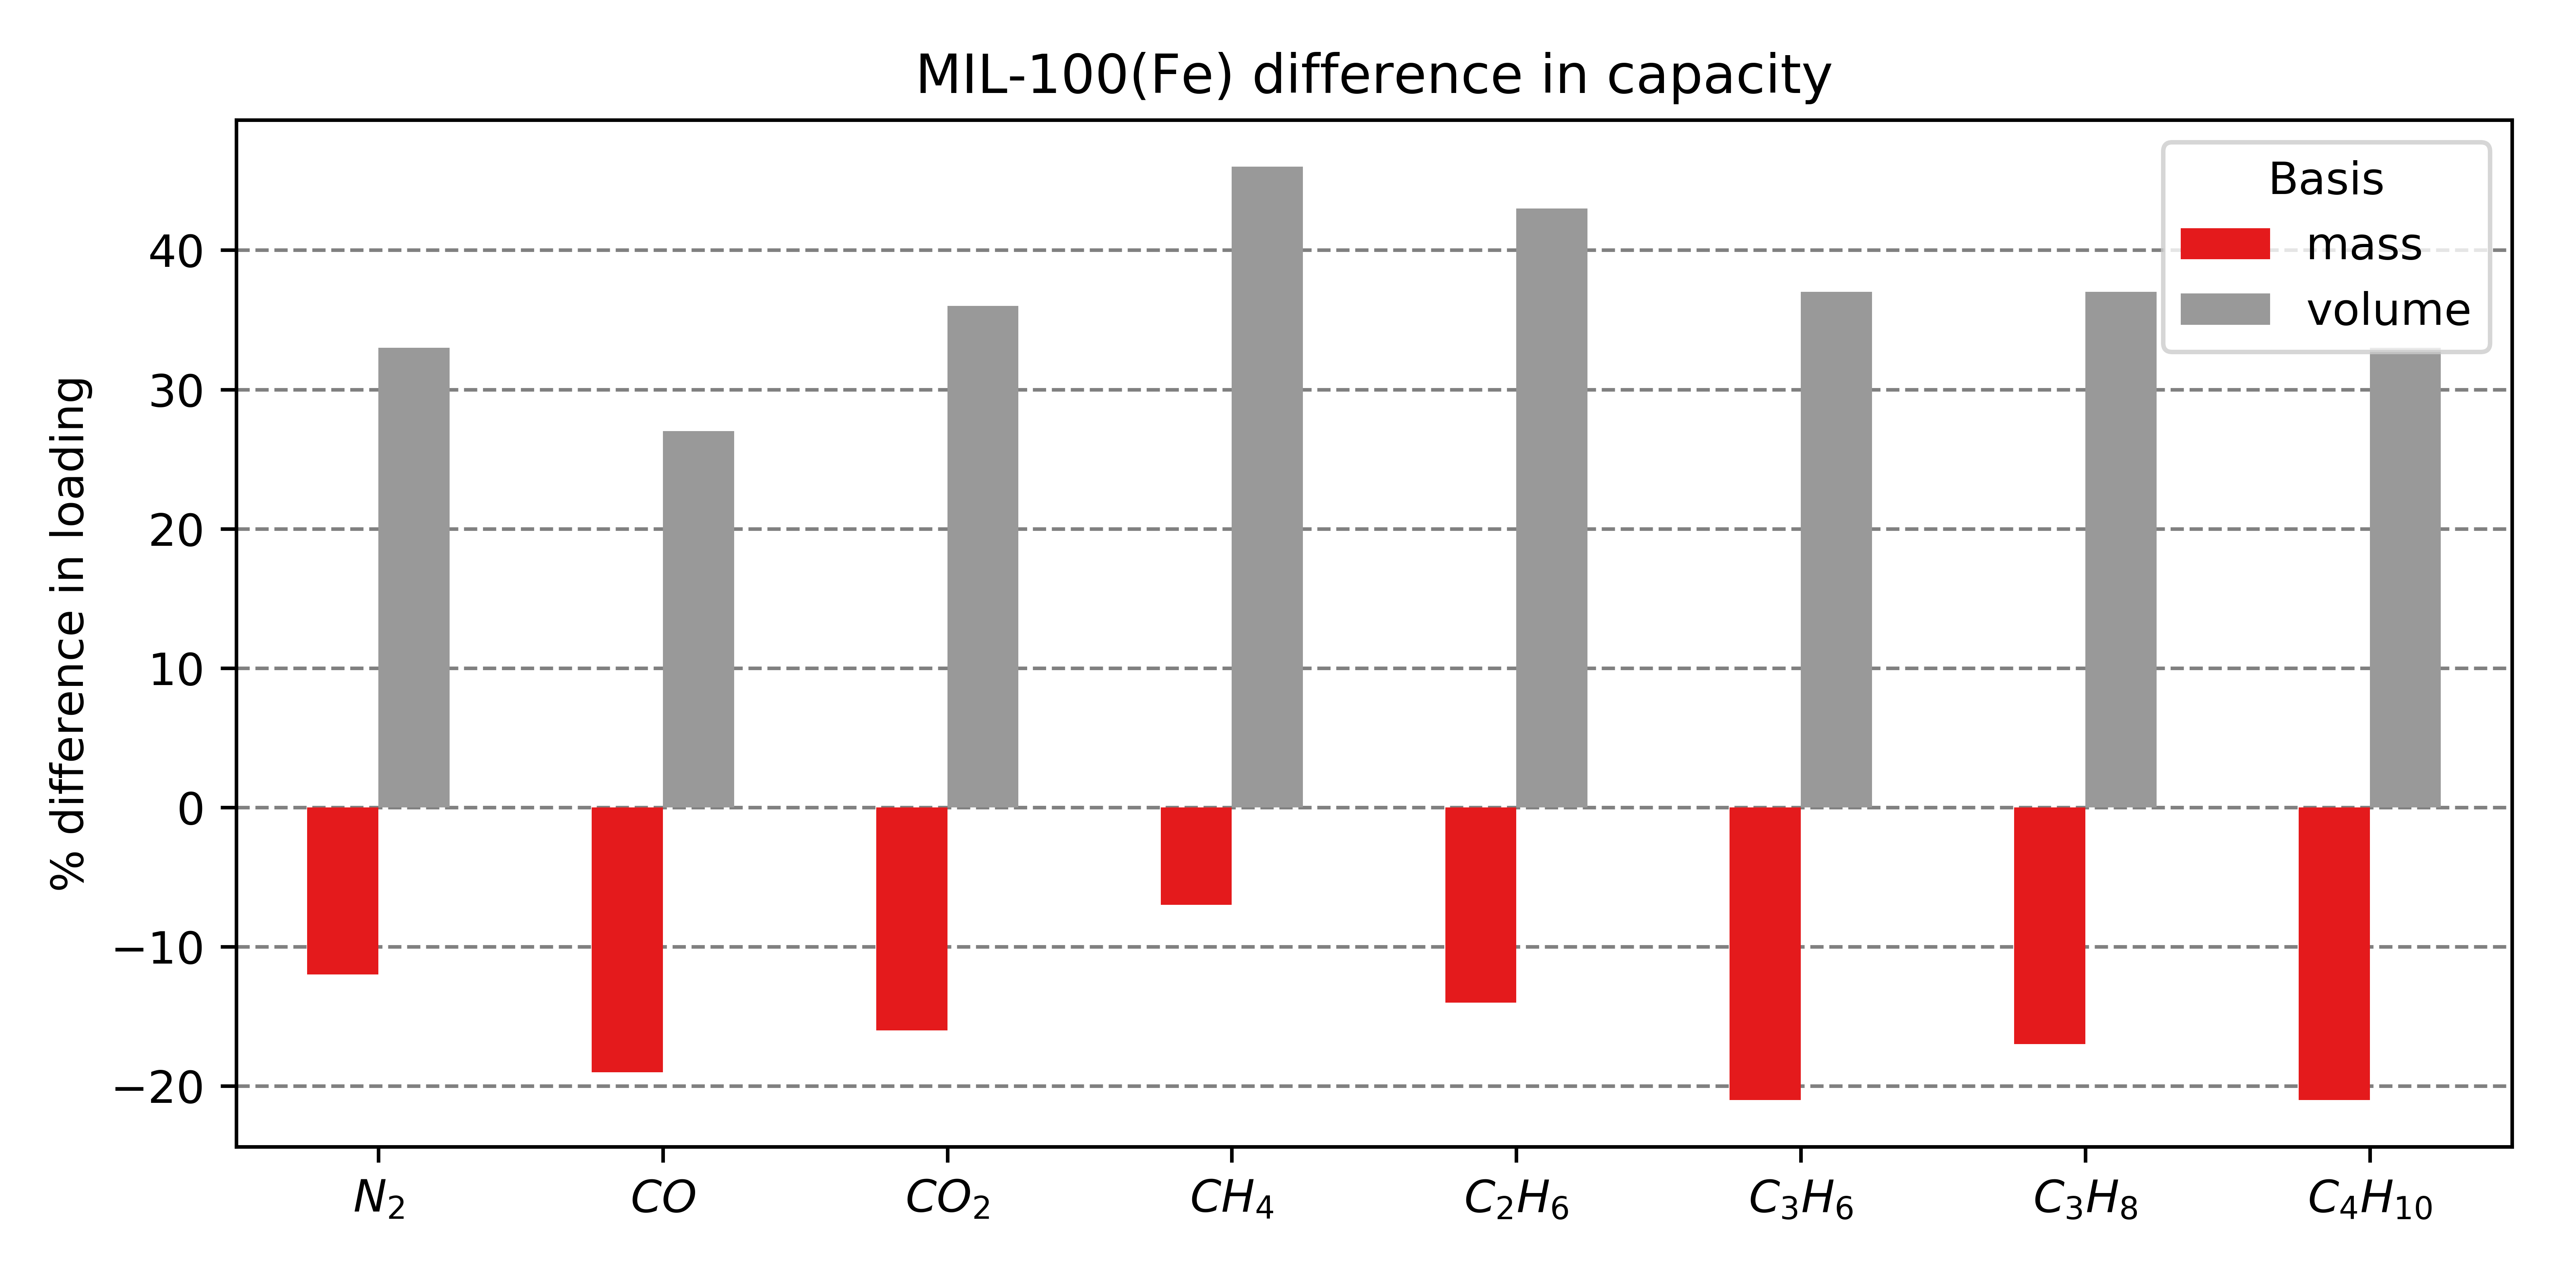
\includegraphics[width=\linewidth]{MIL-100(Fe)-mass-volume}%
		}%
	\end{subfigure}%

	\caption{\glspl{KPI} extracted from the MIL-100(Fe) adsorption dataset with
		(a) logarithmic initial Henry constant (b) initial enthalpy of
		adsorption and (c) change in adsorption maximum capacity from the powder
		to the alumina shaped version on a mass and volume basis in red and grey
		respectively}%
	\label{shaping:fig:analysismil100}
\end{figure}

The enthalpy profiles on the MIL-100(Fe) powder are less homogenous
than the ones on UiO-66(Zr). Some effects can be seen with probes which
can interact with the partially reduced \ce{Fe(II)} atom, such as
carbon monoxide and propylene (\autoref{shaping:fig:mil100isotherms}).
Indeed, when comparing both the initial Henry constants and
enthalpy of adsorption, for \ce{CO} and \ce{C3H6}, these are
higher than the values obtained on UiO-66(Zr).
With initial enthalpy of adsorption for \ce{CO} of around
\SI{45}{\kilo\joule\per\mol}, the value falls into the range of
previous results~\cite{yoonControlledReducibilityMetalOrganic2010}
for interactions with such \ce{Fe(II)} \gls{CUS}.

\begin{figure}[htb]
	\centering
	\begin{subfigure}{0.45\textwidth}
		\includegraphics[width=\linewidth]{calo/MIL-100(Fe)/c3h6-mass-basis-iso}
		\caption{}%
		\label{shaping:fig:mil100c3h6adsmol}
	\end{subfigure}%
	\begin{subfigure}{0.45\textwidth}
		\includegraphics[width=\linewidth]{calo/MIL-100(Fe)/c3h6-volume-basis-iso}
		\caption{}%
		\label{shaping:fig:mil100c3h6adsvol}
	\end{subfigure}%
	\caption{Propylene isotherms on MIL-100(Fe) on a (a) mass
		and (b) volume adsorbent basis.}%
	\label{shaping:fig:mil100isotherms}
\end{figure}

Comparing the powder and shaped variants, there are no
apparent differences between the two. The only discrepancy,
which can be seen on the nitrogen \gls{kH0} follows
as a result of an ill-fitting virial parameter,
and can be assumed an error after observing the isotherm
overlap directly. It could be theorised that by activation at
a higher temperature (\SI{250}{\degreeCelsius}),
the percentage of iron trimers which would undergo reduction will
increase and a more pronounced interaction could be observed.
However, the activation temperature was chosen to allow
comparisons with the \gls{PVA} study~\cite{chanutObservingEffectsShaping2016},
where temperatures over \SI{180}{\degreeCelsius} would lead to the
burn-off of the polymer binder.

The maximum loading differences (\autoref{shaping:fig:analysismil100basis})
of MIL-100(Fe) show a very similar behaviour.
On all probes tested, a fixed capacity
loss of between 10-20\% can be seen on a mass
basis. However, the increase in density afforded by the
compression during pelletisation leads to a compensation in
performance as can be seen directly when looking at isotherms on mass and
volume material basis in \autoref{shaping:fig:mil100c3h6adsmol} and
\autoref{shaping:fig:mil100c3h6adsvol} respectively.

We can conclude that MIL-100(Fe) is almost unaffected by alumina shaping.
A slight loss in maximum capacity on a mass basis is compensated by a pronounced densification, which is desirable in an industrial setting.

% !TEX root = ../../main.tex

\subsubsection{MIL-127(Fe)}

The isotherms on the original powder form of MIL-127(Fe)
should show similar behaviour as on MIL-100(Fe),
due to the presence of the same iron trimesate moieties,
although with a sharper uptake as a result of the smaller pores. Enthalpy
profiles are also influenced by the similar interactions with the iron
\gls{CUS} leading to higher initial heats of adsorption on \ce{CO} and \ce{C3H6}.
An overall increase in the enthalpy of adsorption at higher loadings is seen
throughout the probe series, as seen for example on butane in
\autoref{shaping:fig:mil127c4h10ads}.
Due to the bimodal pore distribution in the MIL-127(Fe) structure,
it is likely that adsorption first commences in the small
(\( \sim \)\SI{0.6}{\nano\metre}) channels and then, at higher pressures,
intrusion into the larger cage-type pores is possible through the
\( \sim \)\SI{0.3}{\nano\metre} narrow apertures.
The confined cages have an increased interaction with the molecule
which leads to the higher enthalpy values.

When comparing the powder and the pellet variant with respect to
initial Henry's constant, a large difference in \gls{kH0} on \ce{CO}
stands out. The value of the initial enthalpy of adsorption
does not follow the same pattern.
However, visual inspection of the enthalpy curve in
\autoref{shaping:fig:mil127coads} shows that the energy of
adsorption corresponding to
interactions with the more active sites is maintained for a \textit{larger
percentage of the total coverage}.
This points to the higher preponderence of such sites in the powder
variant. A similar offset can be seen in the propylene enthalpy at very
low pressures, through it is not reflected in the shape of the isotherm.
The weaker complexation strength and the larger size of the molecule
likely limits the effect seen in the carbon monoxide isotherm.
As for the underlying reason behind the isotherm divergence, it
could be that the alumina binder acts as protection against the
generation of iron (II) during thermal activation.
No other differences are seen between the two forms on either Henry
constant and initial enthalpy of adsorption.

\begin{figure}[!htb]
	\centering
	\begin{subfigure}{0.45\textwidth}
		\includegraphics[width=\linewidth]{calo/MIL-127(Fe)/c4h10-mass-basis-log-iso}
		\caption{\ce{C4H10} adsorption isotherms}%
		\label{shaping:fig:mil127c4h10ads}
	\end{subfigure}%
	\begin{subfigure}{0.45\textwidth}
		\includegraphics[width=\linewidth]{calo/MIL-127(Fe)/co-enth}
		\caption{CO adsorption isotherms}%
		\label{shaping:fig:mil127coads}
	\end{subfigure}%
	\caption{Selected isotherms from the MIL-127(Fe) dataset}%
	\label{shaping:fig:mil127isotherms}
\end{figure}

The capacity comparison in \autoref{shaping:fig:analysismil127basis}
paints an interesting picture. For most probes there is no change in
maximum loading showing that there is no structure degradation or
pore filling. Two outliers are apparent: carbon monoxide and
butane. The decrease in capacity on \ce{CO} can be explained through the
aforementioned changes in active site prevalence.
The drop in butane cannot be a consequence of the same effect
as there is a perfect overlap in the enthalpy curves as seen in
\autoref{shaping:fig:mil127c4h10ads}.
Therefore it likely better explained through a size exclusion
effect similar to UiO-66(Zr).

\begin{figure}[p!]
	\centering
	\begin{subfigure}{\linewidth}
		\parbox[c]{0.1\linewidth}{\caption{}%
			\label{shaping:fig:analysismil127henry}}%
		\parbox[b]{0.8\linewidth}{%
			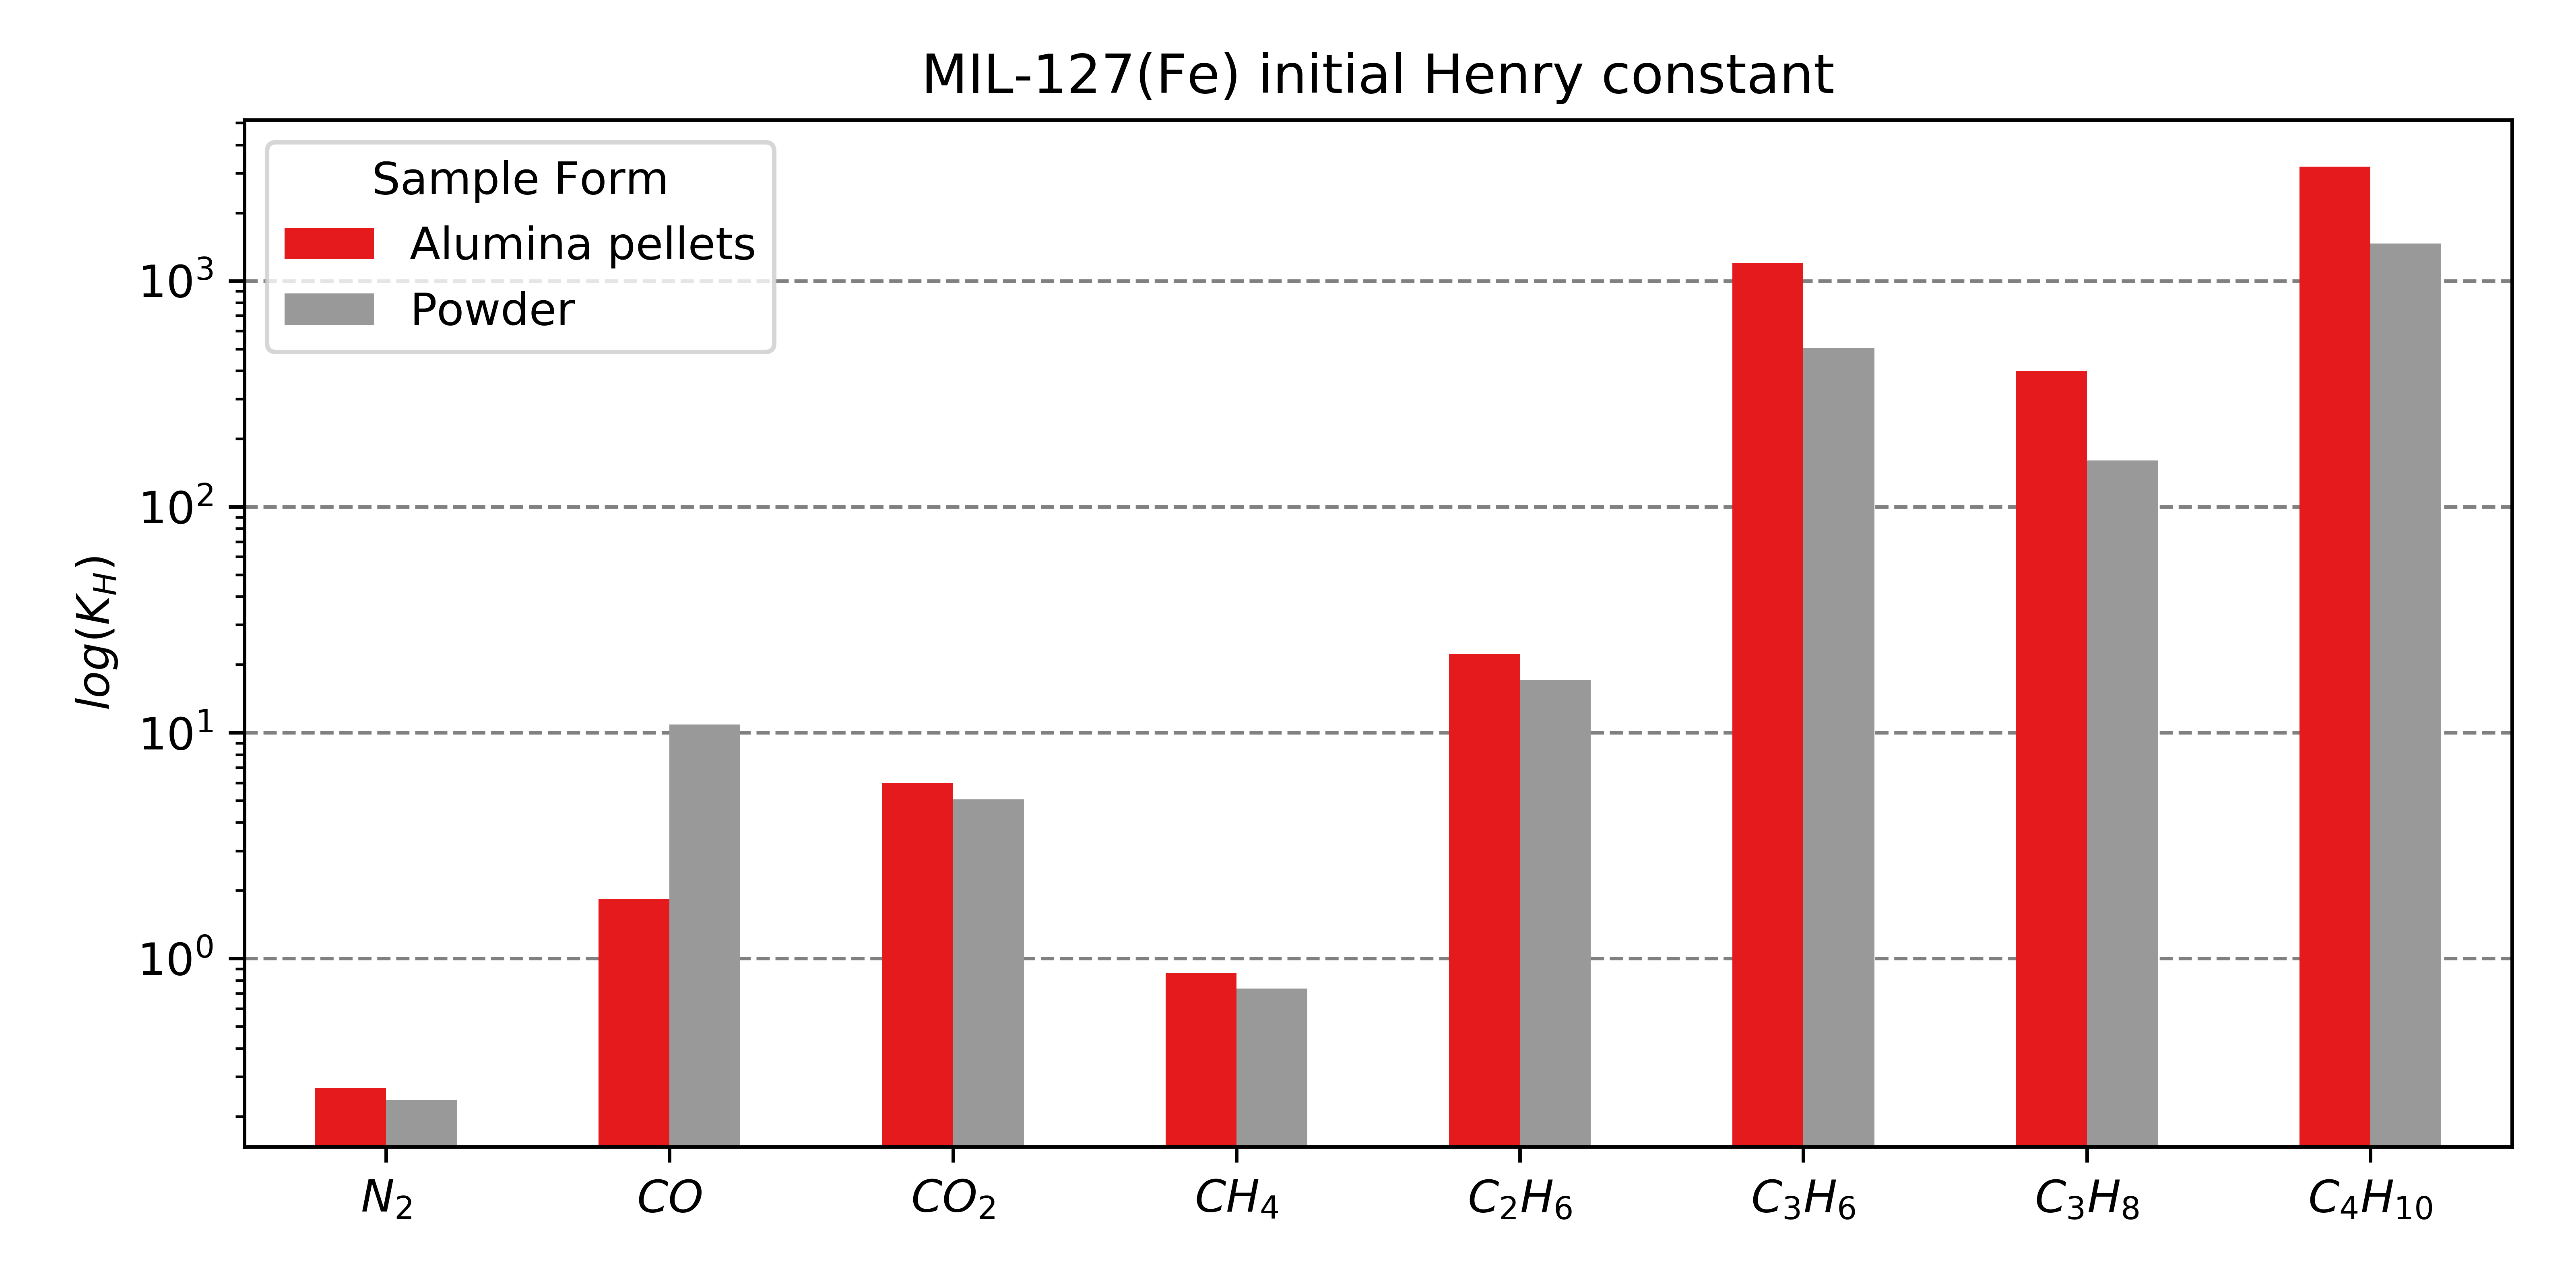
\includegraphics[width=\linewidth]{MIL-127(Fe)-henry-distribution}%
		}%
	\end{subfigure}%

	\begin{subfigure}{\linewidth}
		\parbox[c]{0.1\linewidth}{\caption{}%
			\label{shaping:fig:analysismil127enth}}%
		\parbox[b]{0.8\linewidth}{%
			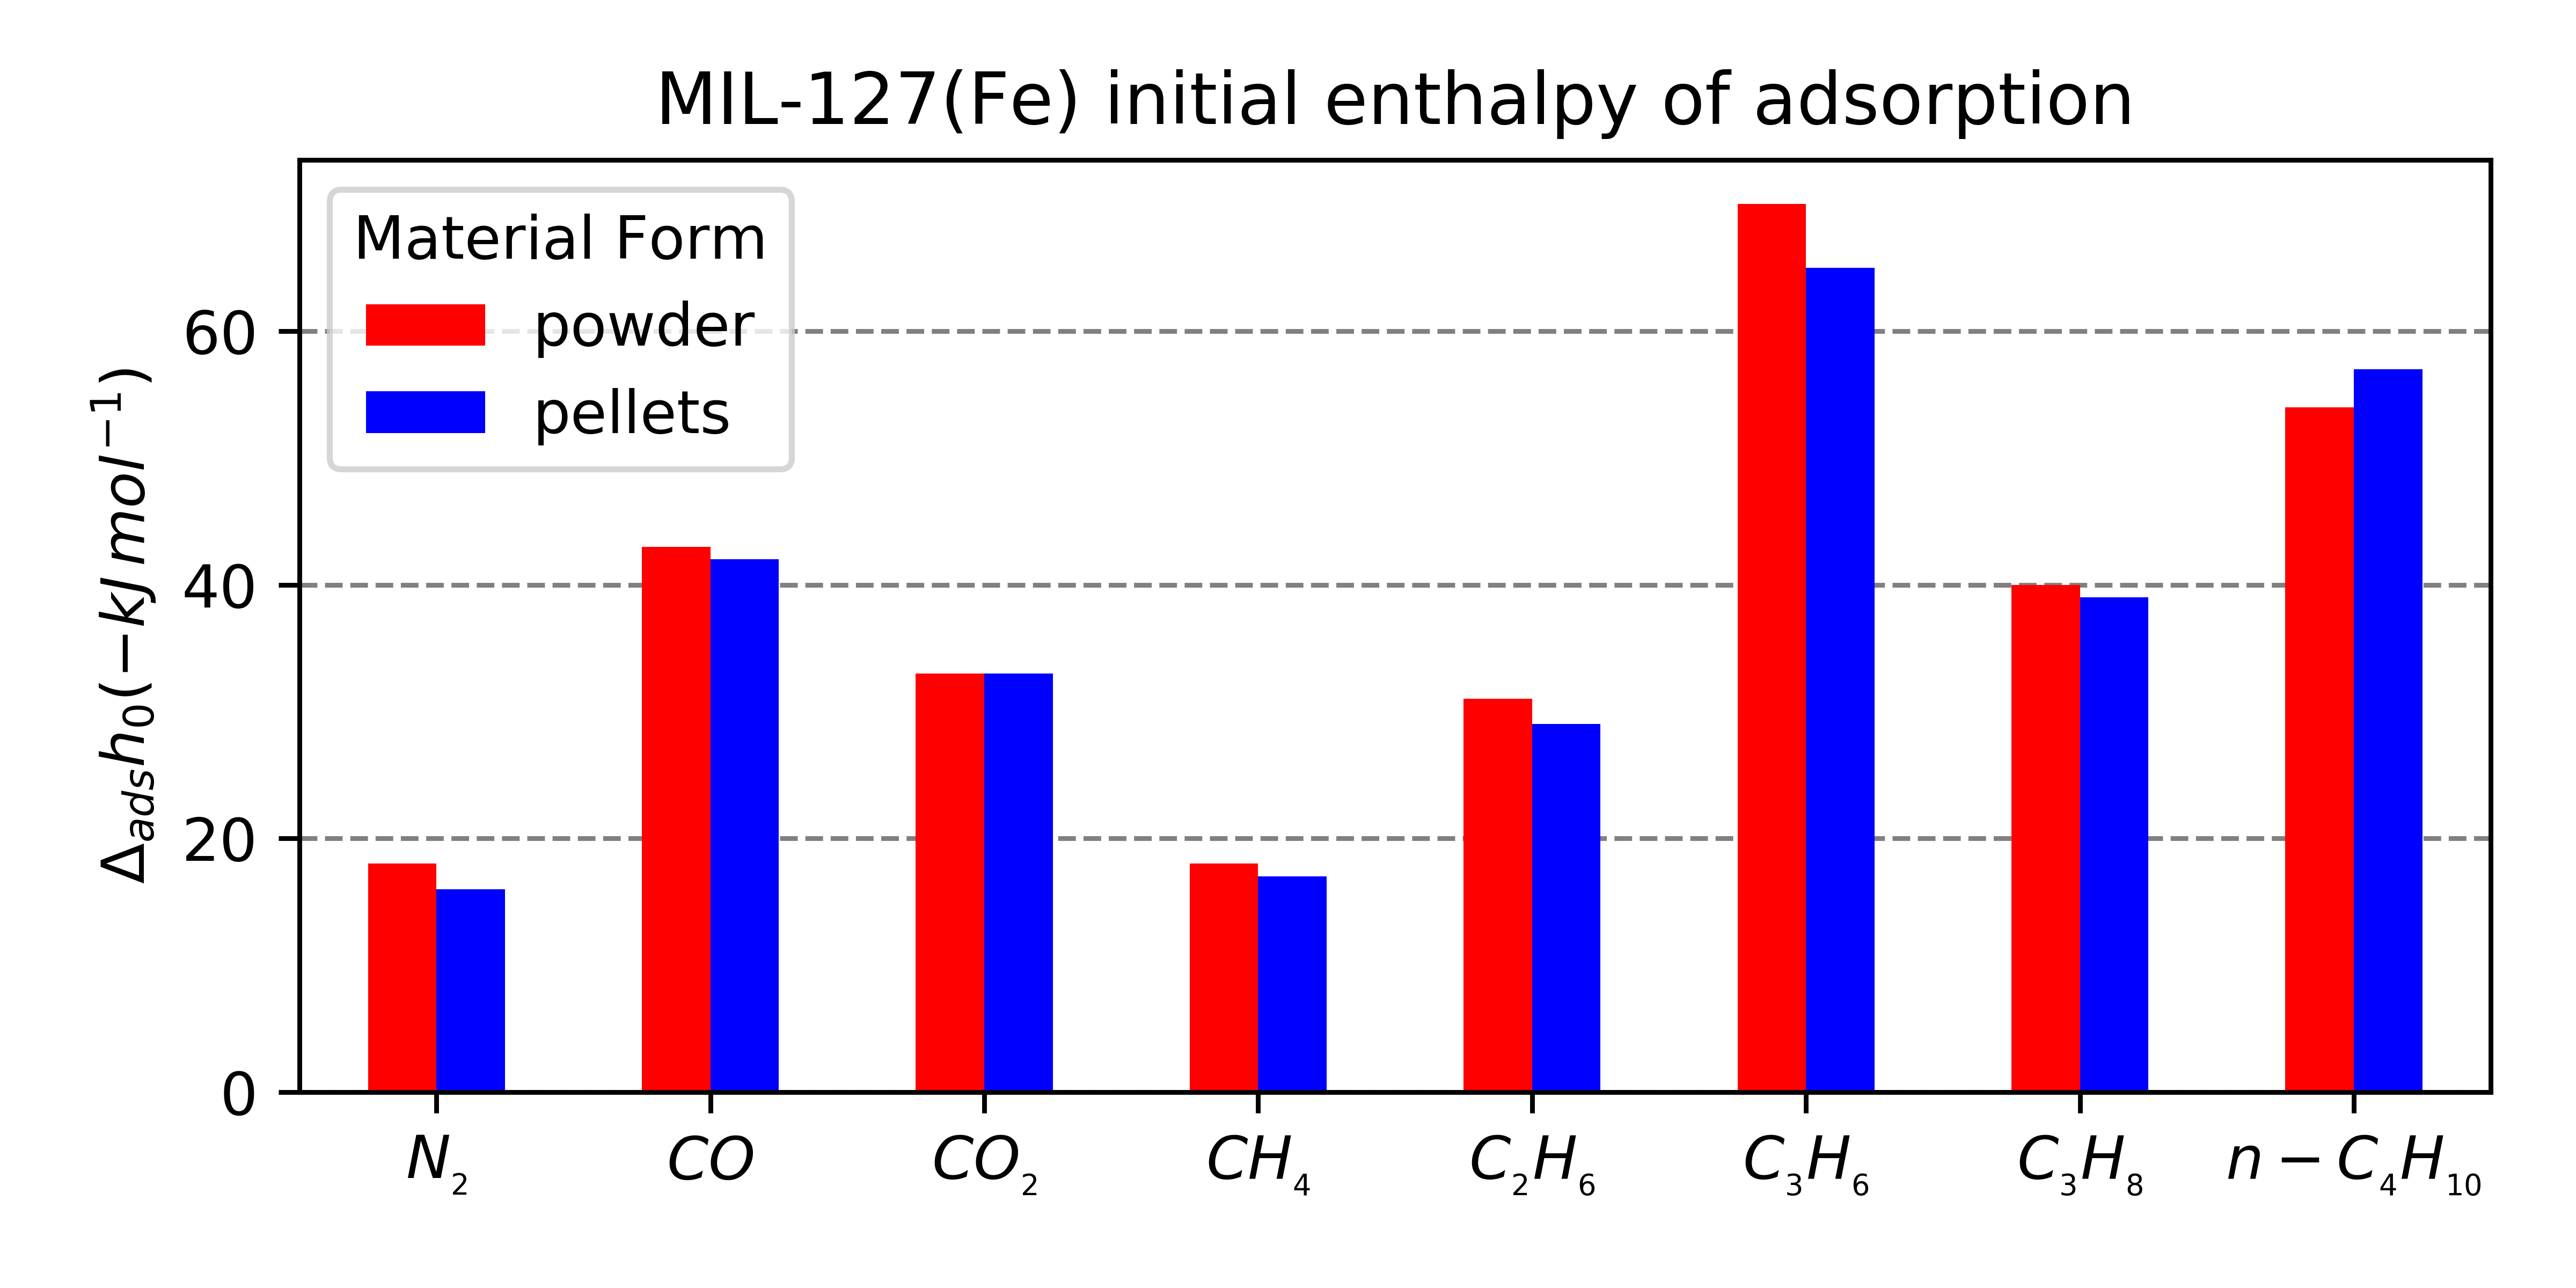
\includegraphics[width=\linewidth]{MIL-127(Fe)-enthalpy-distribution}%
		}%
	\end{subfigure}%

	\begin{subfigure}{\linewidth}
		\parbox[c]{0.1\linewidth}{\caption{}%
			\label{shaping:fig:analysismil127basis}}%
		\parbox[b]{0.8\linewidth}{%
			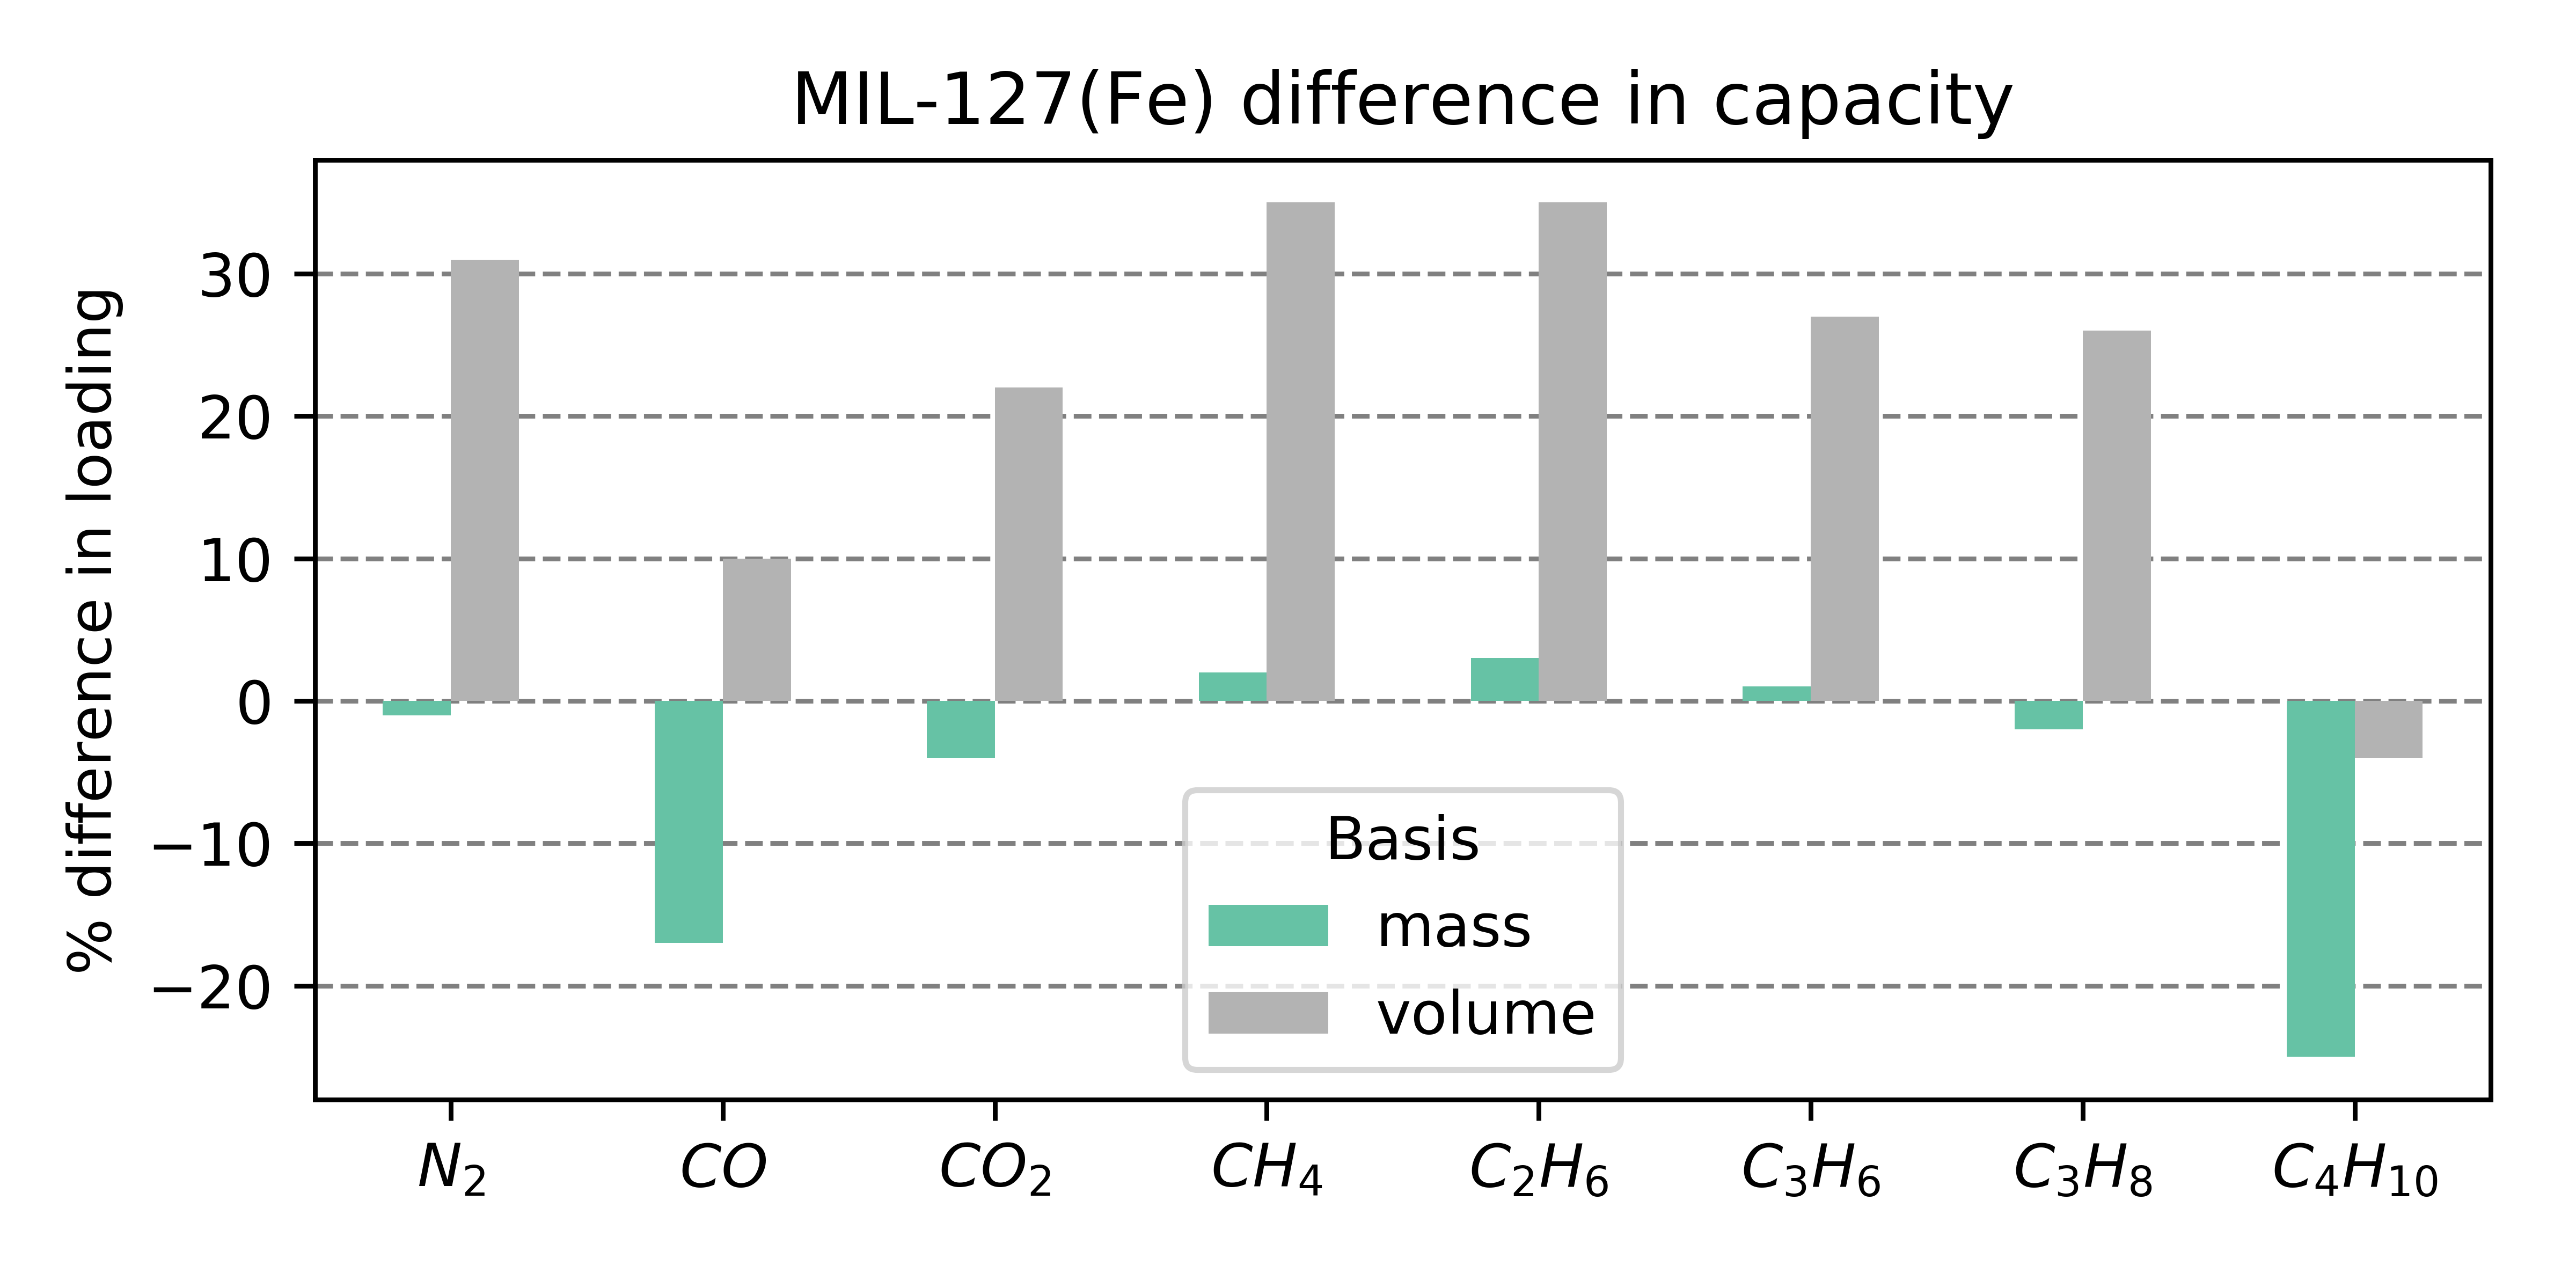
\includegraphics[width=\linewidth]{MIL-127(Fe)-mass-volume}%
		}%
	\end{subfigure}%

	\caption{\glspl{KPI} extracted from the MIL-127(Fe) adsorption dataset with
		(a) logarithmic initial Henry constant (b) initial enthalpy of
        adsorption and (c) change in adsorption maximum capacity from 
        the powder to the alumina shaped version on a mass and volume 
        basis in red and grey respectively}%
	\label{shaping:fig:analysismil127}
\end{figure}

Overall, MIL-127(Fe) shows excellent performance when undergoing
alumina shaping, with almost no capacity loss, as long as
carbon monoxide or butane adsorption are not the required probes,
where specific effects come into play.


% !TEX root = ../../main.tex

\subsection{Vapour adsorption}

The effects of shaping with \(\rho\)-alumina are 
so far more subtle than the changes encountered when using 
\gls{PVA}, as shown in the corresponding 
study~\cite{chanutObservingEffectsShaping2016}.
As such the characterisation was extended using adsorption
of vapours at room temperature.
The influence of the binder on hydrophobic character of the
material may be of interest for tuning the properties of the 
beads. Here, water and methanol
can serve as probes for small changes in surface properties.
To this end, the same \gls{PVA} samples which were 
used in the previous study were investigated alongside 
the \gls{MRA}-shaped \gls{MOF}.

Due to its surface charges, alumina is a 
hydrophilic substance, with a contact 
angle of \SI{10}{\degree}. It is expected that its 
addition may therefore increase the affinity 
of the resulting pellet towards water. On the other hand,
the \gls{PVA} binder is more hydrophobic, with a water contact
angle of \SI{51}{\degree}. The medium affinity for water
is due to the surface hydroxyl functionalisations, which
can lead to hydrogen bonding.

\begin{figure}[p!]
    \centering
    
    \begin{subfigure}{\linewidth}
        \centering
        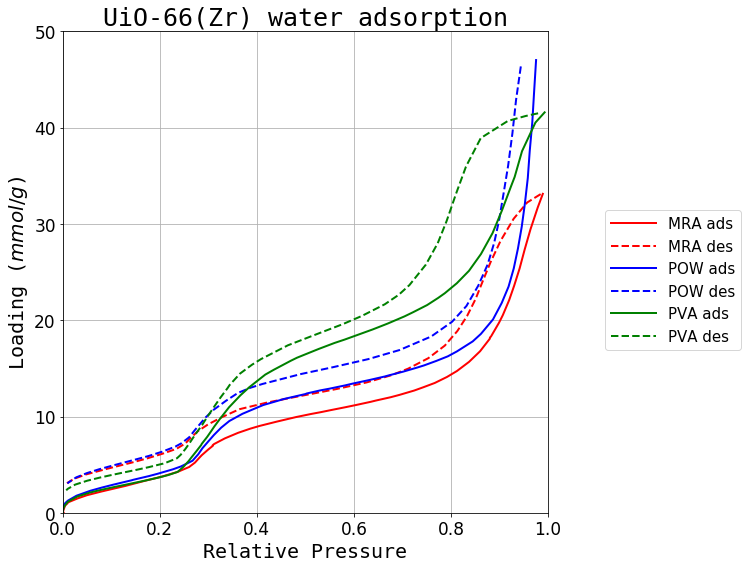
\includegraphics[width=0.45\textwidth]{water/UiO-66(Zr)-water}%
        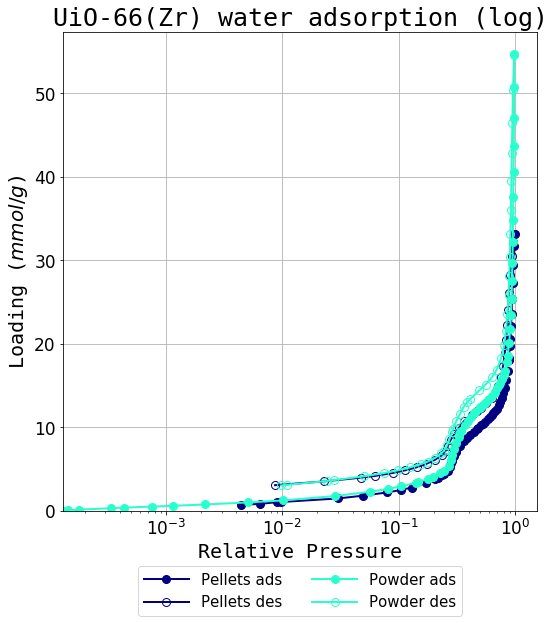
\includegraphics[width=0.45\textwidth]{water/UiO-66(Zr)-water-log}%
        \caption{}\label{shaping:fig:wateruio66}
    \end{subfigure}%

    \begin{subfigure}{\linewidth}
        \centering
        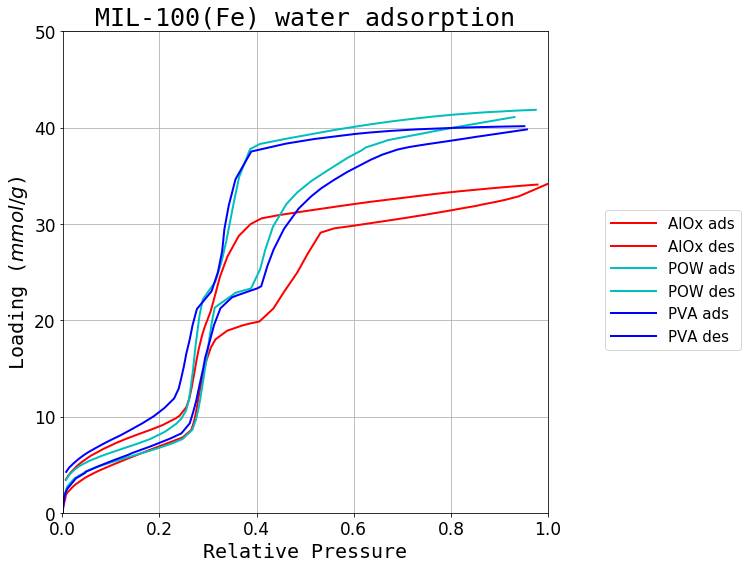
\includegraphics[width=0.45\textwidth]{water/MIL-100(Fe)-water}%
        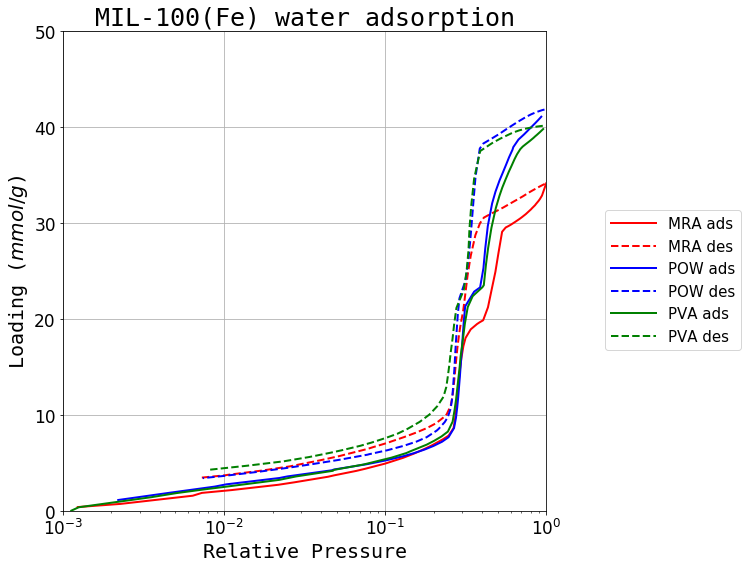
\includegraphics[width=0.45\textwidth]{water/MIL-100(Fe)-water-log}%
        \caption{}\label{shaping:fig:watermil100}
    \end{subfigure}%

    \begin{subfigure}{\linewidth}
        \centering
        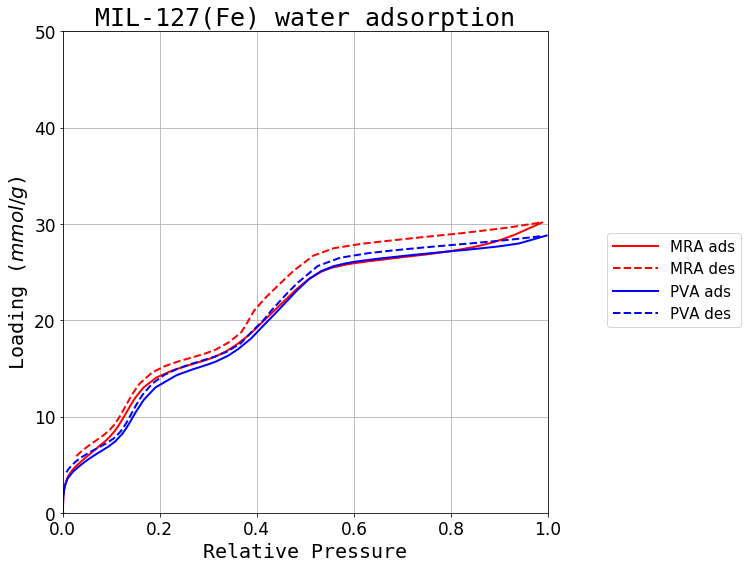
\includegraphics[width=0.45\textwidth]{water/MIL-127(Fe)-water}%
        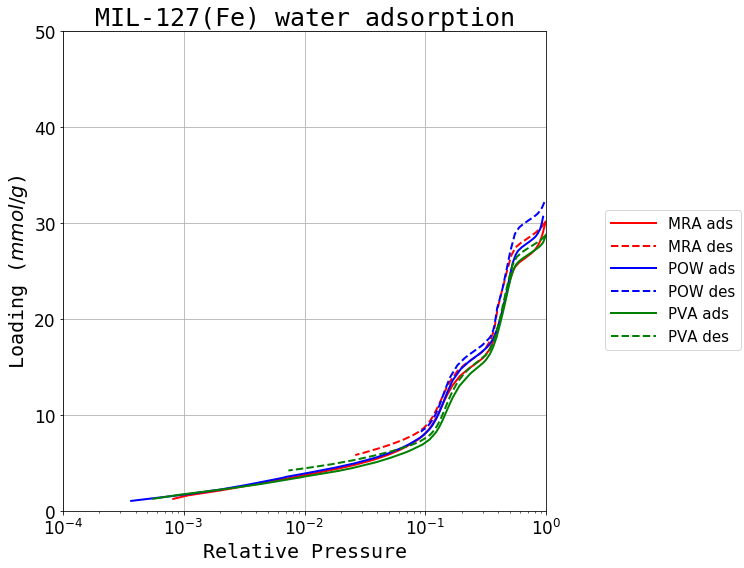
\includegraphics[width=0.45\textwidth]{water/MIL-127(Fe)-water-log}%
        \caption{}\label{shaping:fig:watermil127}%
    \end{subfigure}%
    
    \caption{Water adsorption isotherms (a) UiO-66(Zr), 
    (b) MIL-100(Fe) and (c) MIL-127(Fe). The powder samples are in light
    blue, while the \(\rho\)-alumina and poly-vinyl alcohol samples are
    in red and dark blue respectively. Logarithmic graphs of the
    isotherms are on the right for clarity of the low
    pressure region.}%
    \label{shaping:fig:wateradsorption}
\end{figure}

Two visual indicators may highlight changes in material hydrophilicity: 
the slope of the isotherm in the low relative pressure region 
(\(p/p_0 < 0.3\)) and condensation steps in the isotherm. 
Adsorption at low pressures is representative of the initial
interactions with the surface, as discussed in the previous section.
The pressure at which condensation occurs in the pores of the material, 
underlined by a sharp increase in the isotherm, depends on the 
size of the pore but also on pore environment and 
guest-guest interactions. Finally, hysteresis in the adsorption 
isotherm may also be an indication of the nature of pores.

The measured isotherms on water and methanol can be found
in \autoref{shaping:fig:wateradsorption} 
and \autoref{shaping:fig:methanoladsorption} respectively.
Initial Henry constants \gls{kH0} have been calculated for the isotherms
using the initial point method, and are displayed in
\autoref{shaping:fig:vapourkh}.

\begin{figure}[htb]
    \centering
    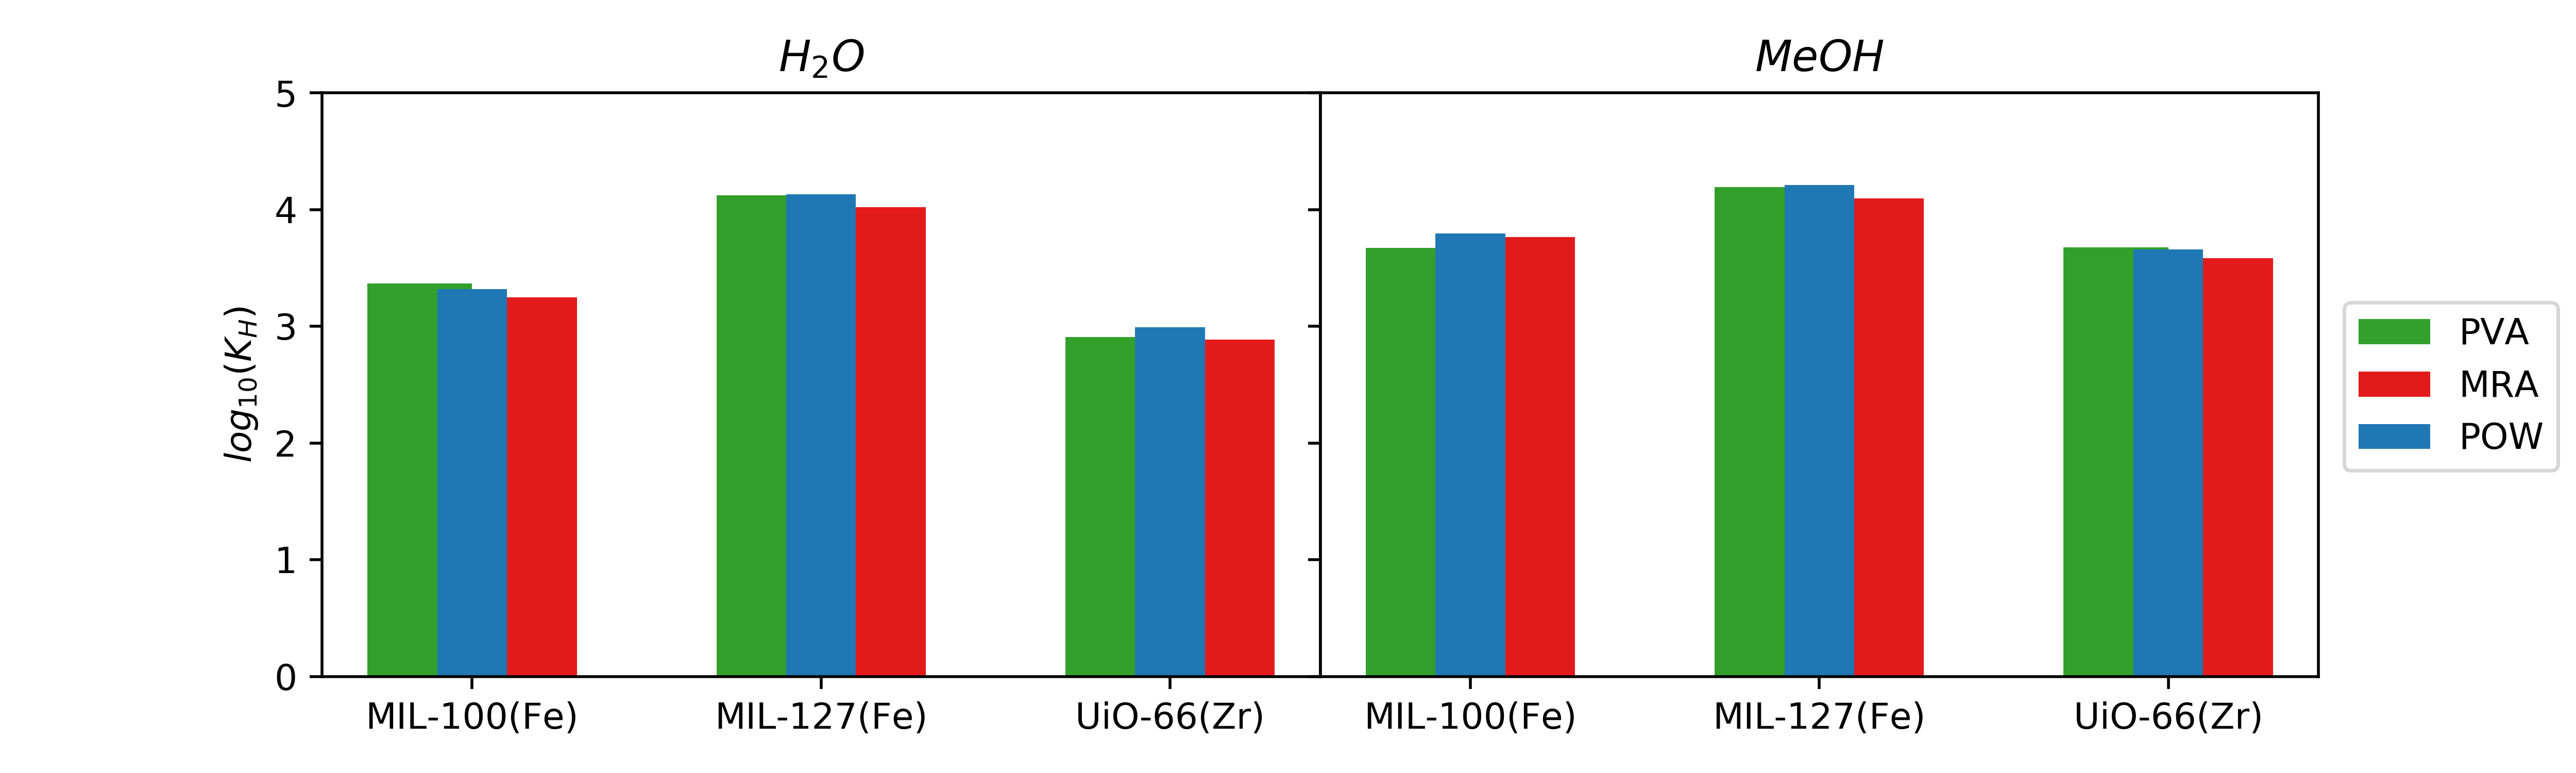
\includegraphics[width=\linewidth]{vapourkh}%
    \caption{Calculated initial Henry constant for
    the vapour adsorption isotherms 
    in \autoref{shaping:fig:wateradsorption}
    and \autoref{shaping:fig:methanoladsorption}}%
    \label{shaping:fig:vapourkh}
\end{figure}

\begin{figure}[p!]
    \centering

    \begin{subfigure}{\linewidth}
        \centering
        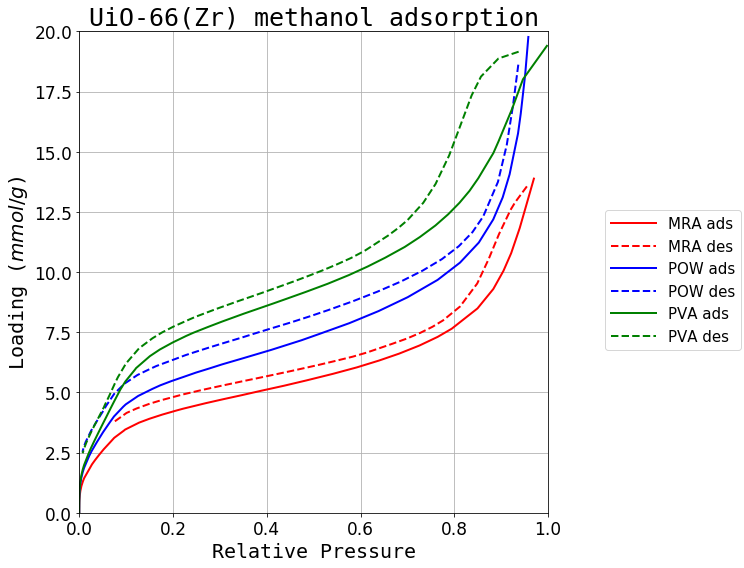
\includegraphics[width=0.45\textwidth]{methanol/UiO-66(Zr)-methanol}%
        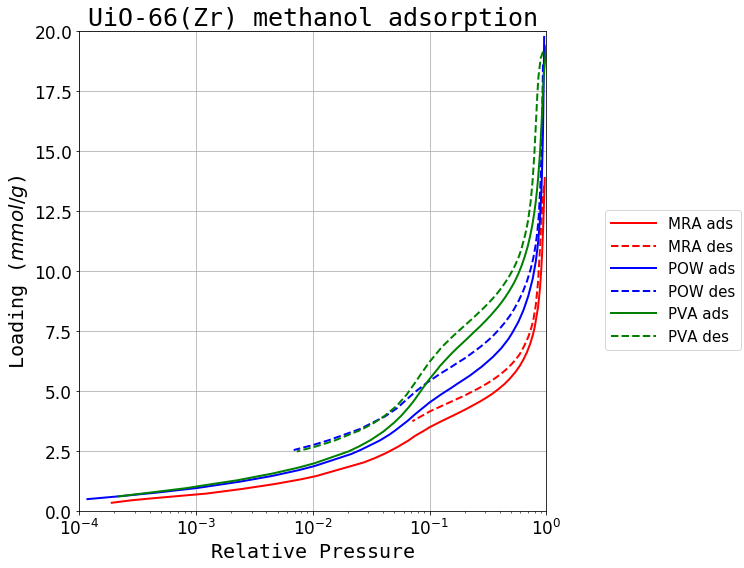
\includegraphics[width=0.45\textwidth]{methanol/UiO-66(Zr)-methanol-log}%
        \caption{}\label{shaping:fig:methanoluio66}%
    \end{subfigure}%

    \begin{subfigure}{\linewidth}
        \centering
        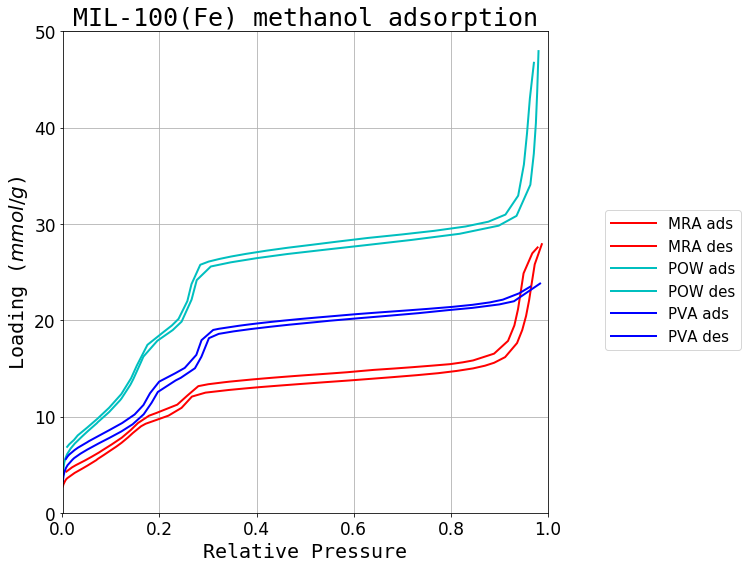
\includegraphics[width=0.45\textwidth]{methanol/MIL-100(Fe)-methanol}%
        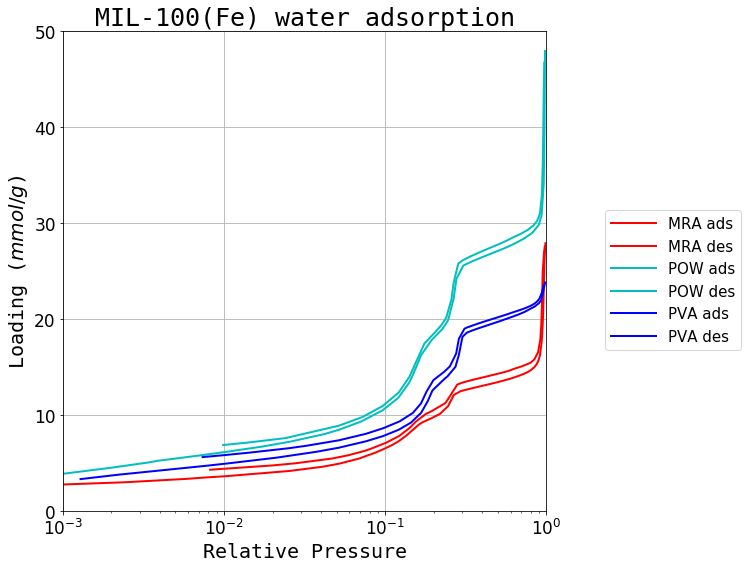
\includegraphics[width=0.45\textwidth]{methanol/MIL-100(Fe)-methanol-log}%
        \caption{}\label{shaping:fig:methanolmil100}%
    \end{subfigure}%

    \begin{subfigure}{\linewidth}
        \centering
        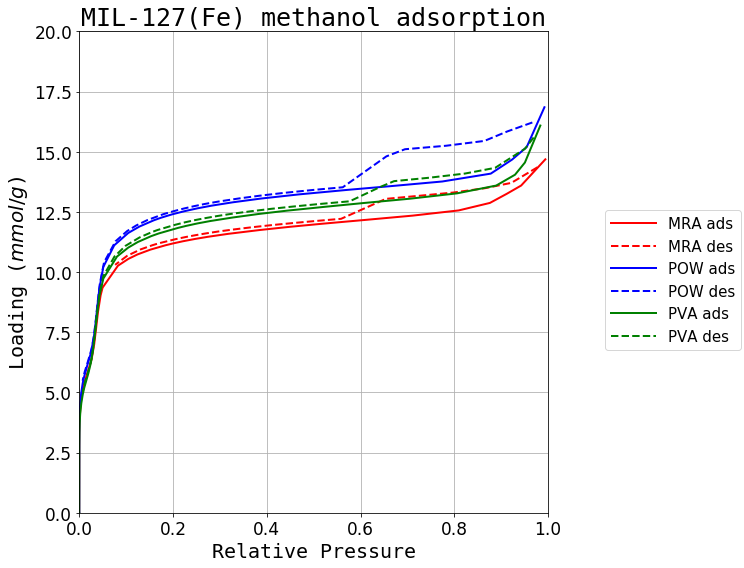
\includegraphics[width=0.45\textwidth]{methanol/MIL-127(Fe)-methanol}%
        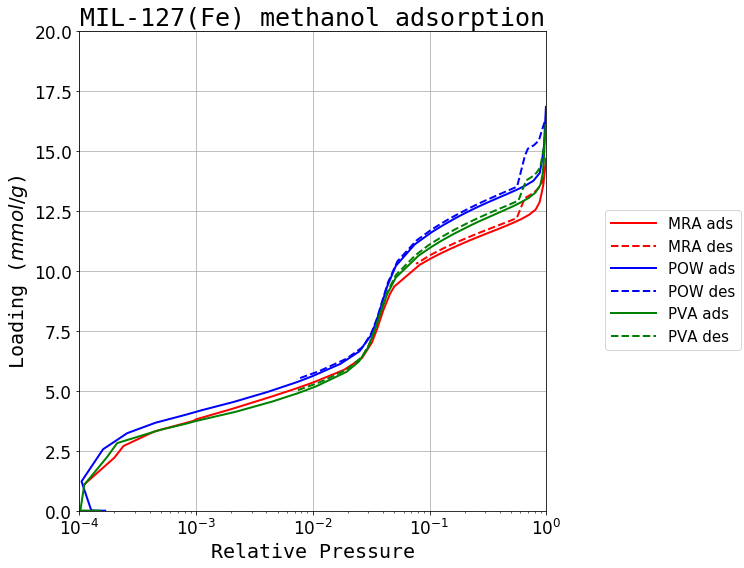
\includegraphics[width=0.45\textwidth]{methanol/MIL-127(Fe)-methanol-log}%
        \caption{}\label{shaping:fig:methanolmil127}%
    \end{subfigure}%
    
    \caption{Methanol adsorption isotherms (a) UiO-66(Zr), 
    (b) MIL-100(Fe) and (c) MIL-127(Fe). The powder samples are in light
    blue, while the \gls{MRA} and \gls{PVA} samples are in red
    and dark blue respectively. Logarithmic 
    graphs of the isotherms are on the right for clarity of the low
    pressure region.}%
    \label{shaping:fig:methanoladsorption}
\end{figure}

\subsubsection{UiO-66(Zr)}

On the parent UiO-66(Zr), the water isotherm shows a slow uptake 
at the start, indicating a hydrophobic surface, and then shows 
a small step at \(p/p_0 = 0.3\). While little is 
adsorbed on the \gls{MOF} before this step, its presence 
at a low relative humidity is indicative of intrinsic defects
in the framework~\cite{ghoshWaterAdsorptionUiO662014}.
Complete saturation takes place around \(p/p_0 = 0.9\). 
A wide hysteresis curve can be seen, which 
does not fully close, even at low pressures. Both the
saturation step and the condensation may be attributed 
to agglomeration of crystals and interparticle voids.

The methanol isotherm has the same features as the water
one, with the condensation step shifted at a much lower 
partial pressure (\(10^{-1} p/p_0\)). It is likely that
the organic component of methanol interacts with the
hydrophobic surface, thus permitting pore filling at
lower pressures. This is also evidenced through the higher
Henry constant when compared to water.

When comparing the powder and the pellet variants, the 
general shape of the isotherm remains the same with both
water and methanol. Initial interactions with the surface are also
identical, as evidenced by the overlap in the low pressure region
and through the calculated Henry constants. The isotherms 
begin to diverge after the condensation step, where the 
maximum loading evolves in the order \gls{MRA} < powder < \gls{PVA}
for both vapours. This is a surprising trend, as both pellets
have been shown to have lower capacities than the powder,
stemming from material amorphization during granulation.
The addition of hydrophilic alumina conforms to this hypothesis,
and appears to have no impact on the initial interaction with 
the surface. On the other hand, polymer-shaped particles
seem to have a higher maximum capacity than both powder and 
alumina pellets. It is unclear if this effect is due to a 
cooperative effect of hydrogen bonding with hydroxyl groups 
on the polymer chains or has another underlying cause.


\subsubsection{MIL-100(Fe)}

The water isotherm on the powder MIL-100(Fe) material show a more 
hydrophilic environment, with a higher initial uptake, and two 
condensation steps at \(p/p_0 = 0.3\) and \(p/p_0 = 0.5\).
At low pressures, adsorption takes place on metal sites in the 
large cages, with clusters formed around these hydrophilic
sites. The two steps correspond to the successive filling of the 
\SI{2.5}{\nano\metre} and the \SI{2.9}{\nano\metre} pores. The
adsorption and desorption branches show a hysteresis loop 
formation, associated with the condensation in the largest 
mesoporous spherical pore.

The methanol isotherm on the same parent \gls{MOF} still presents 
two condensation steps, which have been shifted to a
lower pressure. There is no longer any hysteresis present,
an indication that the critical pore radius for its formation
is not attained when using methanol.

If comparing the powder isotherms with their shaped counterparts,
no differences in features are visible. Initial Henry's constant 
is similar with all  

\subsubsection{MIL-127(Fe)}

On the last \gls{MOF} powder, the water isotherm shows a hydrophilic
surface, with a highest initial slope out of the three 
materials studied. The isotherm has two condensation steps,
a low relative humidity one at \(0.15~p/p_0\), which corresponds
to the filling of the hydrophilic pore, and a condensation 
step situated at \(0.5~p/p_0\) inside the more hydrophobic micropore.
No hysteresis is observed.

As a striking difference from water behaviour, methanol adsorption
leads to completely filled pores at below \(0.15\) relative 
pressure. By examining the logarithmic isotherms in 
\autoref{shaping:fig:methanolmil127} a steep slope at low
pressures is evident. It is likely that the larger size of the
methanol molecule is much more affected by confinement in 
the hydrophilic pore, and leads to sudden micropore filling.
The same effect, combined with the increased affinity for the 
organic part of the probe is likely responsible for shifting the 
secondary condensation step at lower pressures.

The similarities between the both variants of shaped pellets 
and the original powder confirms the previously observed 
suitability of this \gls{MOF} towards the shaping process. The isotherms
overlap almost fully, with a slight difference in maximum uptake
in the order of powder > \gls{PVA} > alumina.